% !TeX program = xelatex
% !TeX encoding = UTF-8
% Presentazione revisionata: Tellus: R e gestione dei dati
% Basata sul materiale originale fornito dall'autore e sul template M01_Pensare_con_i_dati.tex
% Compilazione: xelatex -interaction=nonstopmode Tellus_M02_gestione_dati.tex (due passaggi)
% Diagrammi, tabelle e grafici sono incorporati nel sorgente come codice TikZ.
% Revisione completa delle 83 slide; fonti consultate il 18 novembre 2026.
\documentclass[12pt,aspectratio=1610]{beamer}
\geometry{paperwidth=20cm,paperheight=12.5cm}
\usepackage[italian,provide=*]{babel}
\usepackage{fontspec}
\IfFontExistsTF{NimbusSans-Regular.otf}{
\setsansfont{NimbusSans-Regular.otf}[BoldFont=NimbusSans-Bold.otf,ItalicFont=NimbusSans-Italic.otf,BoldItalicFont=NimbusSans-BoldItalic.otf]
\setmainfont{NimbusSans-Regular.otf}[BoldFont=NimbusSans-Bold.otf,ItalicFont=NimbusSans-Italic.otf,BoldItalicFont=NimbusSans-BoldItalic.otf]
}{
\setsansfont{TeX Gyre Heros}
\setmainfont{TeX Gyre Heros}
}
\IfFontExistsTF{DejaVu Sans Mono}{
\setmonofont{DejaVu Sans Mono}[Scale=.88]
}{\setmonofont{Latin Modern Mono}[Scale=.88]}
\usefonttheme{professionalfonts}
\usepackage{amsmath,amssymb,booktabs,array,graphicx,tikz,bookmark}
\usetikzlibrary{calc,positioning,arrows.meta}
\graphicspath{{Risorse/Figure/}}
\definecolor{Paper}{HTML}{F8F6F1}
\definecolor{Ink}{HTML}{253344}
\definecolor{Navy}{HTML}{15283E}
\definecolor{Quantum}{HTML}{5146A5}
\definecolor{Classical}{HTML}{087C74}
\definecolor{Muted}{HTML}{657180}
\definecolor{Rule}{HTML}{D6DAD9}
\definecolor{Night}{HTML}{112236}
\definecolor{Lilac}{HTML}{ABB5FF}
\definecolor{Mint}{HTML}{72D8C8}
\setbeamercolor{background canvas}{bg=Paper}
\setbeamercolor{normal text}{fg=Ink}
\setbeamertemplate{navigation symbols}{}
\setbeamertemplate{headline}{}
\setbeamertemplate{footline}{}
\setbeamersize{text margin left=0pt,text margin right=0pt}
\hypersetup{colorlinks=true,linkcolor=Classical,urlcolor=Classical,pdfpagemode=UseOutlines,pdfstartview=Fit,
 pdftitle={Tellus: R e gestione dei dati},pdfauthor={Marzio De Corato},
 pdfsubject={Modulo M02: importazione, trasformazioni e controlli, Revisione completa: diagrammi TikZ, formule e codice R commentato}}
\bookmarksetup{open,openlevel=0,depth=2}
\newsavebox{\BodyBox}
\newsavebox{\SideBox}
\newsavebox{\RecallBox}
\newsavebox{\TitleBox}
\newcommand{\MeasureBox}[2]{\typeout{REVIEWBOX:#1:\the\wd#2:\the\ht#2:\the\dp#2}}

% Revisione completa: diagrammi TikZ, formalismo e box R.
\usepackage[most]{tcolorbox}
\usepackage{listings}
\usetikzlibrary{fit,backgrounds,matrix,decorations.pathreplacing}
\definecolor{GeoA}{HTML}{1D7890}
\definecolor{GeoB}{HTML}{C57E42}
\definecolor{GeoC}{HTML}{7363AA}
\definecolor{GeoTint}{HTML}{F0F4F3}
\lstdefinestyle{GeoR}{language=R,basicstyle=\ttfamily\fontsize{9.2}{12.2}\selectfont,
 keywordstyle=\color{Quantum}\bfseries,commentstyle=\color{Classical},stringstyle=\color{GeoB},
 numbers=left,numberstyle=\tiny\color{Muted},numbersep=4pt,showstringspaces=false,
 columns=fullflexible,keepspaces=true,breaklines=true,xleftmargin=1.15em,
 frame=none,aboveskip=0pt,belowskip=0pt,tabsize=2}
\newsavebox{\PilotLeftBox}
\newsavebox{\PilotRightBox}
\newcommand{\PLabel}[1]{\par{\color{Classical}\bfseries\fontsize{9}{11}\selectfont\MakeUppercase{#1}}\par\vspace{1.8mm}}
\newcommand{\PBody}[1]{\par{\fontsize{11.3}{14.8}\selectfont #1\par}}
\newcommand{\PSmall}[1]{\par{\fontsize{9.8}{13.1}\selectfont #1\par}}
\newcommand{\PCode}[2]{%
\begin{tcolorbox}[enhanced,arc=1.8mm,boxrule=.65pt,
  colback=white,colframe=Classical!75!Navy,colbacktitle=Navy,
  coltitle=white,fonttitle=\bfseries\fontsize{9.6}{12}\selectfont,
  title={#1},left=1.7mm,right=1.3mm,top=1.5mm,bottom=1.3mm,
  before skip=1mm,after skip=1mm]
\lstinputlisting[style=GeoR]{Codice/#2}
\end{tcolorbox}}
\newcommand{\PInfo}[1]{%
\begin{tcolorbox}[enhanced,arc=1.6mm,boxrule=.55pt,colback=GeoTint,
 colframe=Rule!80!Classical,left=2.3mm,right=2.3mm,top=2mm,bottom=2mm,
 before skip=1mm,after skip=1mm]
\PSmall{#1}\end{tcolorbox}}
\tikzset{
 pFlow/.style={draw=Classical!45,fill=white,rounded corners=2mm,
  line width=.7pt,align=center,minimum height=1.1cm,font=\sffamily\fontsize{10}{12}\selectfont},
 pEdge/.style={-{Latex[length=2.3mm]},draw=Classical,line width=.95pt},
 pGroup/.style={draw=Rule,fill=white,rounded corners=2mm,line width=.65pt},
 pDotA/.style={circle,fill=GeoA,inner sep=1.25pt},
 pDotB/.style={circle,fill=GeoB,inner sep=1.25pt},
 pDotC/.style={circle,fill=GeoC,inner sep=1.25pt}
}
\newcommand{\PilotChrome}[4]{%
  \node[anchor=north west,inner sep=0,text width=17.7cm] at ([xshift=.95cm,yshift=-.55cm]current page.north west) {\color{Navy}\bfseries\fontsize{20.6}{24.5}\selectfont #1};
  \node[anchor=north east,inner sep=0] at ([xshift=19.05cm,yshift=-.14cm]current page.north west) {\color{Classical}\fontsize{8}{10}\selectfont\hyperlink{slide2}{#2}};
  \draw[Classical,line width=1.2pt] ([xshift=.95cm,yshift=-1.7cm]current page.north west)--([xshift=2.35cm,yshift=-1.7cm]current page.north west);
  \draw[Rule,line width=.65pt] ([xshift=.95cm,yshift=-10.36cm]current page.north west)--([xshift=19.05cm,yshift=-10.36cm]current page.north west);
  \node[anchor=north west,inner sep=0] at ([xshift=.96cm,yshift=-10.55cm]current page.north west) {\color{Classical}\bfseries\fontsize{9.1}{12}\selectfont DA RICORDARE};
  \node[anchor=north west,inner sep=0,text width=14.3cm] at ([xshift=4.2cm,yshift=-10.53cm]current page.north west) {\color{Ink}\fontsize{10.3}{13.8}\selectfont #4};
  \draw[Rule,line width=.35pt] ([xshift=.95cm,yshift=-11.92cm]current page.north west)--([xshift=19.05cm,yshift=-11.92cm]current page.north west);
  \node[anchor=north west,inner sep=0] at ([xshift=.95cm,yshift=-12.06cm]current page.north west) {\color{Muted}\fontsize{7.7}{9.2}\selectfont Tellus: R e gestione dei dati};
  \node[anchor=north east,inner sep=0] at ([xshift=19.05cm,yshift=-12.06cm]current page.north west) {\color{Muted}\fontsize{7.7}{9.2}\selectfont #3/82};
}


% Stili comuni per i diagrammi scientifici della revisione completa.
\tikzset{
 pAxis/.style={-{Latex[length=2mm]},draw=Muted,line width=.65pt},
 pNote/.style={font=\sffamily\fontsize{9}{11.5}\selectfont,text=Muted,align=center},
 pLabel/.style={font=\sffamily\fontsize{10}{12.5}\selectfont,text=Ink,align=center}
}
\newsavebox{\FullWideBox}
\setlength{\emergencystretch}{1em}


\begin{document}

\begin{frame}[plain]\hypertarget{slide1}{}
% Copertina 3D: immagine renderizzata in Blender e titoli LaTeX sovrapposti.
\begin{tikzpicture}[remember picture,overlay]
\fill[Night] (current page.south west) rectangle (current page.north east);
\node[anchor=south west,inner sep=0,outer sep=0] at (current page.south west) {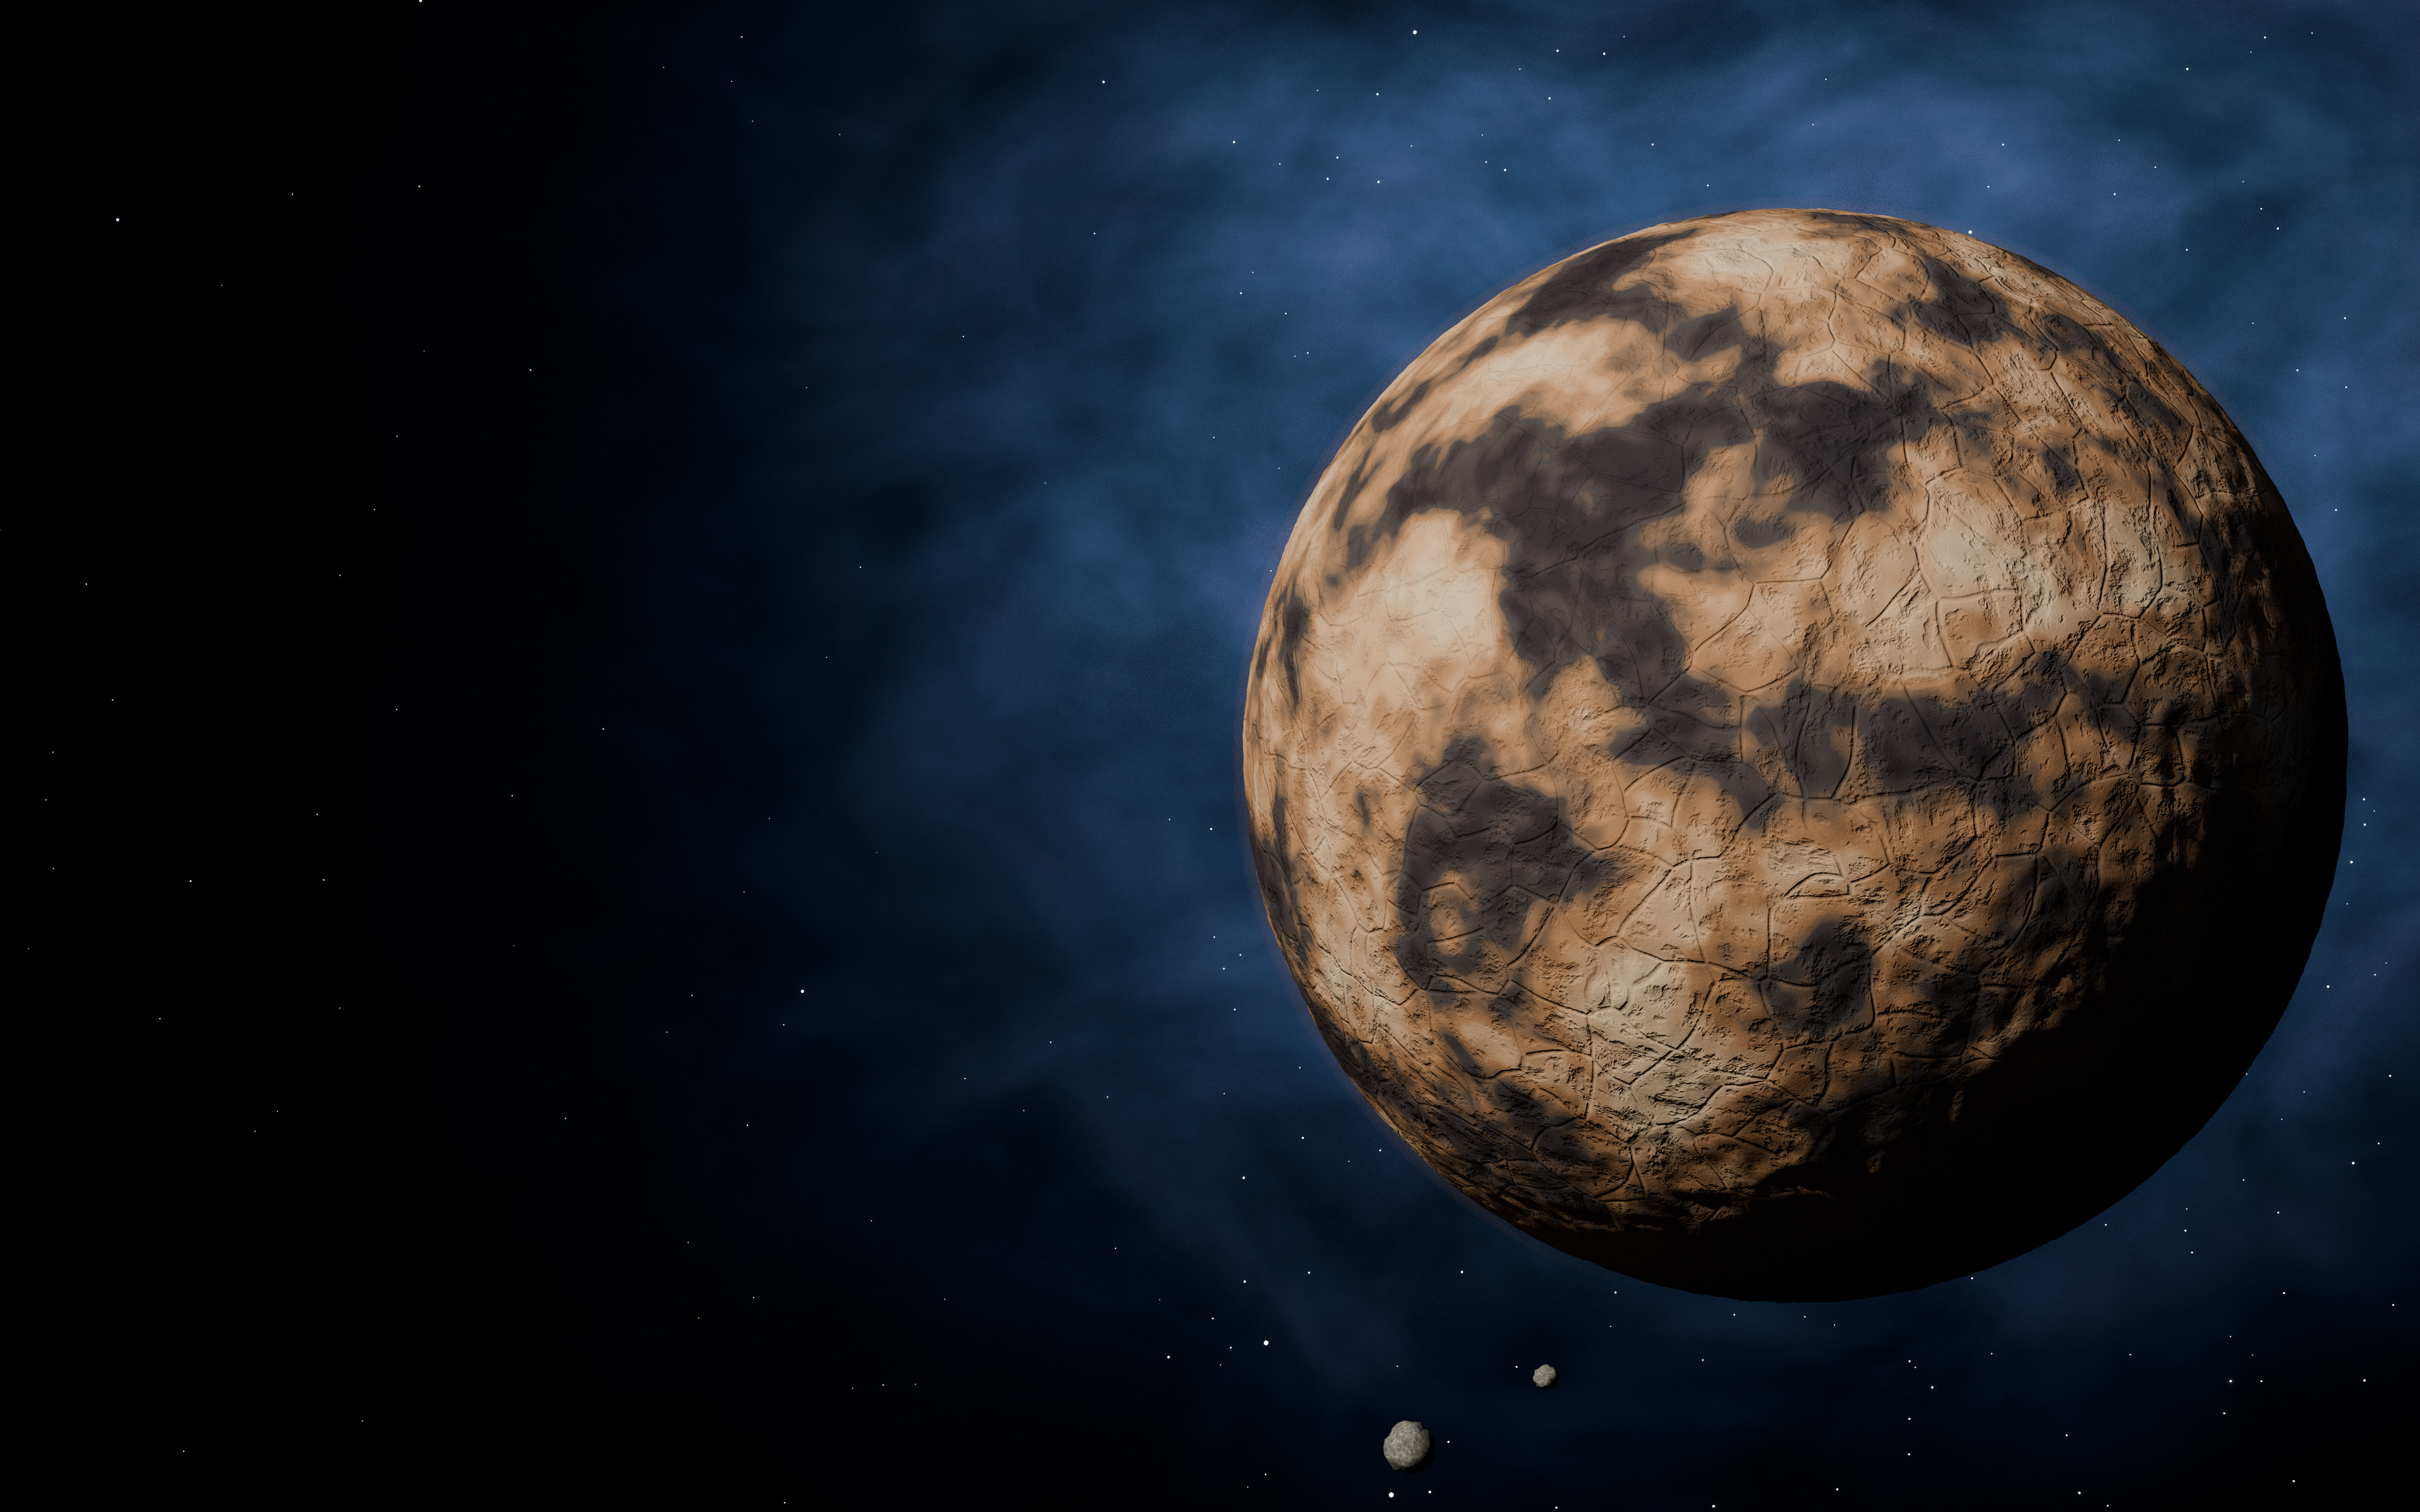
\includegraphics[width=\paperwidth,height=\paperheight]{Risorse/Copertine/M02_Tellus.jpg}};

\node[anchor=north west,inner sep=0,text width=9.2cm] at
 ([xshift=1.05cm,yshift=-1.10cm]current page.north west)
 {\color{Mint}\bfseries\fontsize{23}{27}\selectfont TELLUS};
\node[anchor=north west,inner sep=0,text width=9.2cm] at
 ([xshift=1.07cm,yshift=-2.16cm]current page.north west)
 {\color{white}\fontsize{9.0}{12}\selectfont MODULO M02 · SCIENZE DELLA TERRA};
\draw[Mint,line width=1.4pt] ([xshift=1.05cm,yshift=-2.78cm]current page.north west)--
 ([xshift=2.60cm,yshift=-2.78cm]current page.north west);
\node[anchor=north west,inner sep=0] at
 ([xshift=1.05cm,yshift=-3.35cm]current page.north west)
 {\begin{minipage}{9.2cm}\raggedright\color{white}\bfseries
 \fontsize{30}{36}\selectfont R e gestione\\dei dati\end{minipage}};
\node[anchor=north west,inner sep=0] at
 ([xshift=1.07cm,yshift=-7.88cm]current page.north west)
 {\begin{minipage}{9.0cm}\raggedright\color{Lilac}
 \fontsize{12.2}{17}\selectfont Dall’importazione alla costruzione\\di dati verificabili\end{minipage}};
\node[anchor=north west,inner sep=0,text width=9.2cm] at
 ([xshift=1.07cm,yshift=-10.52cm]current page.north west)
 {\color{white}\fontsize{11.5}{15}\selectfont Marzio De Corato};
\node[anchor=north west,inner sep=0,text width=9.2cm] at
 ([xshift=1.07cm,yshift=-11.17cm]current page.north west)
 {\color{Lilac}\fontsize{8.8}{11}\selectfont \href{https://creativecommons.org/licenses/by-nc-sa/4.0/}{\textcopyright{} 2026 · CC BY-NC-SA 4.0}};
\end{tikzpicture}
\end{frame}


\begin{frame}[plain]\hypertarget{slide2}{}
\bookmark[level=0,page=2]{Domanda centrale}
\begin{tikzpicture}[remember picture,overlay]
\node[anchor=north west,inner sep=0] at ([xshift=.95cm,yshift=-.67cm]current page.north west) {\color{Navy}\bfseries\fontsize{23}{27}\selectfont Quando una tabella è affidabile?};
\draw[Classical,line width=1.4pt] ([xshift=.95cm,yshift=-1.73cm]current page.north west)--([xshift=2.5cm,yshift=-1.73cm]current page.north west);
\node[anchor=north west,inner sep=0,fill=GeoTint,rounded corners=2mm,text width=17.7cm,inner sep=3.5mm] at ([xshift=1.0cm,yshift=-2.26cm]current page.north west) {\color{Navy}\fontsize{14.1}{19}\selectfont Come trasformare misure eterogenee in dati analitici controllabili?};
\node[draw=Rule,line width=.7pt,fill=GeoTint,rounded corners=2.5mm,minimum width=4.8cm,minimum height=2.15cm,text width=4.38cm,align=center,inner sep=3mm] (n0) at ([xshift=4cm,yshift=-6.15cm]current page.north west) {\color{Navy}\bfseries\fontsize{13}{16}\selectfont IMPORTAZIONE\\[2mm]\color{Ink}\normalfont\fontsize{10.5}{14}\selectfont File e unità dichiarate};
\node[draw=Rule,line width=.7pt,fill=Paper,rounded corners=2.5mm,minimum width=4.8cm,minimum height=2.15cm,text width=4.38cm,align=center,inner sep=3mm] (n1) at ([xshift=10cm,yshift=-6.15cm]current page.north west) {\color{Navy}\bfseries\fontsize{13}{16}\selectfont VERIFICA\\[2mm]\color{Ink}\normalfont\fontsize{10.5}{14}\selectfont Chiavi, tipi e assenze};
\node[draw=Rule,line width=.7pt,fill=GeoTint,rounded corners=2.5mm,minimum width=4.8cm,minimum height=2.15cm,text width=4.38cm,align=center,inner sep=3mm] (n2) at ([xshift=16cm,yshift=-6.15cm]current page.north west) {\color{Navy}\bfseries\fontsize{13}{16}\selectfont TABELLA\\[2mm]\color{Ink}\normalfont\fontsize{10.5}{14}\selectfont Trasformazioni tracciabili};
\draw[-{Stealth[length=3.0mm]},draw=Classical,line width=1.45pt] ([xshift=6.65cm,yshift=-6.15cm]current page.north west)--([xshift=7.35cm,yshift=-6.15cm]current page.north west);
\draw[-{Stealth[length=3.0mm]},draw=Classical,line width=1.45pt] ([xshift=12.65cm,yshift=-6.15cm]current page.north west)--([xshift=13.35cm,yshift=-6.15cm]current page.north west);
\node[anchor=north west,inner sep=0,text width=17.9cm] at ([xshift=1.05cm,yshift=-8.25cm]current page.north west) {\color{Classical}\bfseries\fontsize{10.4}{13.4}\selectfont IDEA GUIDA};
\node[anchor=north west,inner sep=0,text width=17.85cm] at ([xshift=1.05cm,yshift=-8.71cm]current page.north west) {\color{Ink}\fontsize{11.9}{16.0}\selectfont Una tabella è verificabile se mantiene identità, provenienza, unità e trasformazioni tracciabili.};
\draw[Rule,line width=.35pt] ([xshift=.95cm,yshift=-11.92cm]current page.north west)--([xshift=19.05cm,yshift=-11.92cm]current page.north west);
\node[anchor=north west,inner sep=0] at ([xshift=.95cm,yshift=-12.06cm]current page.north west) {\color{Muted}\fontsize{7.7}{9.3}\selectfont Tellus · R e gestione dei dati};
\node[anchor=north east,inner sep=0] at ([xshift=19.05cm,yshift=-12.06cm]current page.north west) {\color{Muted}\fontsize{7.7}{9.3}\selectfont 2/82};
\end{tikzpicture}
\end{frame}
% SLIDE 003 | La tabella analitica e i tre casi di Tellus
\begin{lrbox}{\PilotLeftBox}%
\begin{minipage}[t]{10.05cm}\raggedright\color{Ink}\fontsize{11.3}{14.8}\selectfont

\PLabel{Dati didattici del modulo M02}
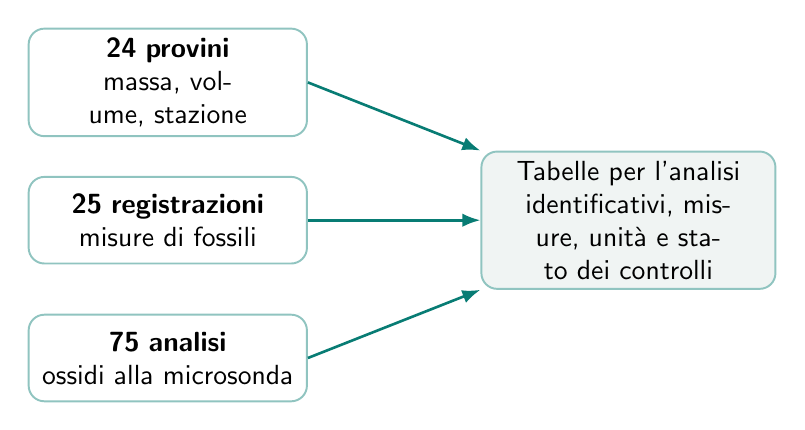
\begin{tikzpicture}[x=1cm,y=1cm]
\node[pFlow,text width=3.3cm] (a) at(1.85,4.3){\textbf{24 provini}\\massa, volume, stazione};
\node[pFlow,text width=3.3cm] (b) at(1.85,2.55){\textbf{25 registrazioni}\\misure di fossili};
\node[pFlow,text width=3.3cm] (c) at(1.85,.8){\textbf{75 analisi}\\ossidi alla microsonda};
\node[pFlow,text width=3.5cm,fill=GeoTint] (t) at(7.7,2.55){Tabelle per l’analisi\\identificativi, misure, unità e stato dei controlli};
\draw[pEdge](a.east)--(t.north west);\draw[pEdge](b)--(t);\draw[pEdge](c.east)--(t.south west);
\end{tikzpicture}
\PBody{I tre casi hanno problemi diversi. Le operazioni conserveranno il legame fra ogni risultato e la registrazione da cui proviene.}

\end{minipage}% 
\end{lrbox}
\begin{lrbox}{\PilotRightBox}%
\begin{minipage}[t]{7.55cm}\raggedright\color{Ink}\fontsize{11.3}{14.8}\selectfont

\PLabel{Il prodotto della lezione}
\PBody{Una tabella analitica contiene le unità e le variabili necessarie per una domanda definita. Le righe selezionate e le quantità derivate devono avere una giustificazione.}
\PInfo{Nel progetto, \texttt{Dati/} conserva i CSV di origine. Gli script producono tabelle derivate e un registro delle decisioni in \texttt{Risultati/}.}
\PSmall{Le osservazioni sono didattiche. Gli esperimenti nel browser usano piccoli dataset propri: ogni attività dichiara il modello e i parametri da confrontare.}

\end{minipage}% 
\end{lrbox}

\begin{frame}[plain]\hypertarget{slide3}{}
\bookmark[level=1,page=3]{La tabella analitica e i tre casi di Tellus}
\begin{tikzpicture}[remember picture,overlay]
\PilotChrome{La tabella analitica e i tre casi di Tellus}{PROGETTO E DATI}{3}{Prima di trasformare una tabella, definire che cosa rappresenta una riga e quale analisi si intende svolgere.}
\node[anchor=north west,inner sep=0] at ([xshift=0.96cm,yshift=-2.13cm]current page.north west) {\usebox{\PilotLeftBox}};
\node[anchor=north west,inner sep=0] at ([xshift=11.52cm,yshift=-2.13cm]current page.north west) {\usebox{\PilotRightBox}};

\end{tikzpicture}\end{frame}

% SLIDE 004 | Cartelle, sorgenti e risultati
\begin{lrbox}{\PilotLeftBox}%
\begin{minipage}[t]{10.05cm}\raggedright\color{Ink}\fontsize{11.3}{14.8}\selectfont

\PLabel{Struttura del progetto distribuito}
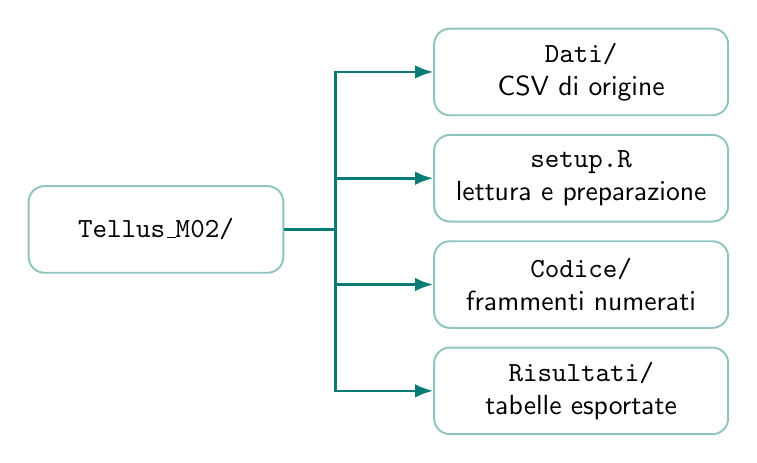
\begin{tikzpicture}[x=1cm,y=1cm]
\node[pFlow,text width=3cm] (r) at(1.7,2){\texttt{Tellus\_M02/}};
\node[pFlow,text width=3.5cm] (d) at(7.1,4){\texttt{Dati/}\\CSV di origine};
\node[pFlow,text width=3.5cm] (s) at(7.1,2.65){\texttt{setup.R}\\lettura e preparazione};
\node[pFlow,text width=3.5cm] (c) at(7.1,1.3){\texttt{Codice/}\\frammenti numerati};
\node[pFlow,text width=3.5cm] (o) at(7.1,-.05){\texttt{Risultati/}\\tabelle esportate};
\foreach \n in {d,s,c,o}{\draw[pEdge] (r.east)--++(.65,0)|-(\n.west);}
\end{tikzpicture}
\PSmall{\texttt{Lezione\_Tellus.R} riunisce i frammenti nell'ordine delle slide. Le risorse della presentazione sono in \texttt{Risorse/}.}

\end{minipage}% 
\end{lrbox}
\typeout{FULLBOX:004:L:\the\ht\PilotLeftBox:\the\dp\PilotLeftBox}
\begin{lrbox}{\PilotRightBox}%
\begin{minipage}[t]{7.55cm}\raggedright\color{Ink}\fontsize{11.3}{14.8}\selectfont

\PCode{R · avviare il progetto}{04_progetto.R}
\PBody{Aprire il file \texttt{.Rproj} imposta la cartella del progetto in RStudio. \texttt{getwd()} mostra la cartella corrente.}
\PSmall{\texttt{setup.R} legge i CSV e prepara gli oggetti comuni. Il suo codice è incluso: conversioni e flag dei fossili vengono ripresi nelle sezioni successive.}

\end{minipage}% 
\end{lrbox}
\typeout{FULLBOX:004:R:\the\ht\PilotRightBox:\the\dp\PilotRightBox}
\begin{frame}[plain]\hypertarget{slide4}{}
\bookmark[level=1,page=4]{Cartelle, sorgenti e risultati}
\begin{tikzpicture}[remember picture,overlay]
\PilotChrome{Cartelle, sorgenti e risultati}{PROGETTO E RIPRODUCIBILITÀ}{4}{I percorsi relativi funzionano quando cartelle distribuite e cartella di lavoro corrispondono.}
\node[anchor=north west,inner sep=0] at ([xshift=0.96cm,yshift=-2.13cm]current page.north west) {\usebox{\PilotLeftBox}};
\node[anchor=north west,inner sep=0] at ([xshift=11.52cm,yshift=-2.13cm]current page.north west) {\usebox{\PilotRightBox}};

\end{tikzpicture}\end{frame}

% SLIDE 005 | Stato della sessione e dipendenze
\begin{lrbox}{\PilotLeftBox}%
\begin{minipage}[t]{10.05cm}\raggedright\color{Ink}\fontsize{11.3}{14.8}\selectfont

\PLabel{Cambiare un parametro non aggiorna un oggetto già calcolato}
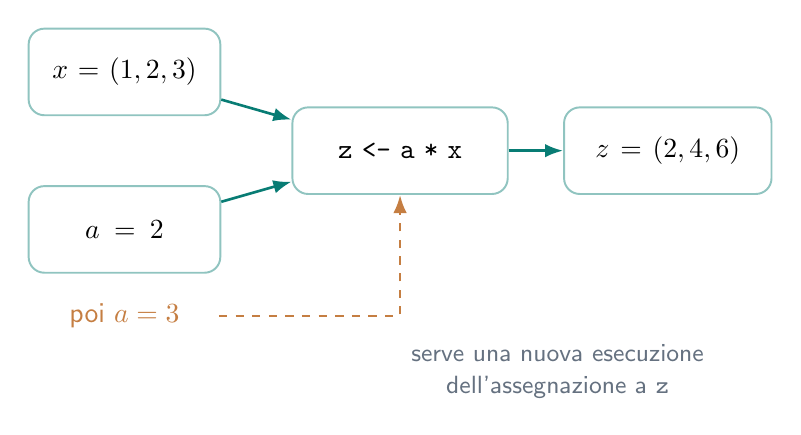
\begin{tikzpicture}[x=1cm,y=1cm]
\node[pFlow,text width=2.2cm] (x) at(1.3,3){$x=(1,2,3)$};
\node[pFlow,text width=2.2cm] (a) at(1.3,1){$a=2$};
\node[pFlow,text width=2.5cm] (f) at(4.8,2){\texttt{z <- a * x}};
\node[pFlow,text width=2.4cm] (z) at(8.2,2){$z=(2,4,6)$};
\draw[pEdge] (x)--(f);\draw[pEdge](a)--(f);\draw[pEdge](f)--(z);
\node[pLabel,text=GeoB] at(1.3,-.1){poi $a=3$};
\draw[pEdge,GeoB,dashed] (2.5,-.1)--(4.8,-.1)--(f.south);
\node[pNote,text width=4.3cm] at(6.8,-.8){serve una nuova esecuzione\\dell'assegnazione a \texttt{z}};
\end{tikzpicture}
\PBody{Il valore conservato in un oggetto dipende dalle istruzioni già eseguite. Il nome di un parametro non crea un collegamento automatico con i risultati.}

\end{minipage}% 
\end{lrbox}
\typeout{FULLBOX:005:L:\the\ht\PilotLeftBox:\the\dp\PilotLeftBox}
\begin{lrbox}{\PilotRightBox}%
\begin{minipage}[t]{7.55cm}\raggedright\color{Ink}\fontsize{11.3}{14.8}\selectfont

\PCode{R · un risultato da ricalcolare}{05_stato.R}
\PSmall{\texttt{1:3} costruisce gli interi da 1 a 3. L'assegnazione conserva il risultato corrente.}
\PInfo{Riavviare la sessione ed eseguire lo script dall'inizio permette di riconoscere le dipendenze assenti dal codice.}

\end{minipage}% 
\end{lrbox}
\typeout{FULLBOX:005:R:\the\ht\PilotRightBox:\the\dp\PilotRightBox}
\begin{frame}[plain]\hypertarget{slide5}{}
\bookmark[level=1,page=5]{Stato della sessione e dipendenze}
\begin{tikzpicture}[remember picture,overlay]
\PilotChrome{Stato della sessione e dipendenze}{PROGETTO E RIPRODUCIBILITÀ}{5}{Un risultato aggiornato richiede di rieseguire tutte le operazioni che dipendono dai parametri modificati.}
\node[anchor=north west,inner sep=0] at ([xshift=0.96cm,yshift=-2.13cm]current page.north west) {\usebox{\PilotLeftBox}};
\node[anchor=north west,inner sep=0] at ([xshift=11.52cm,yshift=-2.13cm]current page.north west) {\usebox{\PilotRightBox}};

\end{tikzpicture}\end{frame}

% SLIDE 006 | Istruzioni nell’ordine delle dipendenze
\begin{lrbox}{\PilotLeftBox}%
\begin{minipage}[t]{10.05cm}\raggedright\color{Ink}\fontsize{11.3}{14.8}\selectfont

\PLabel{Una trasformazione affine}
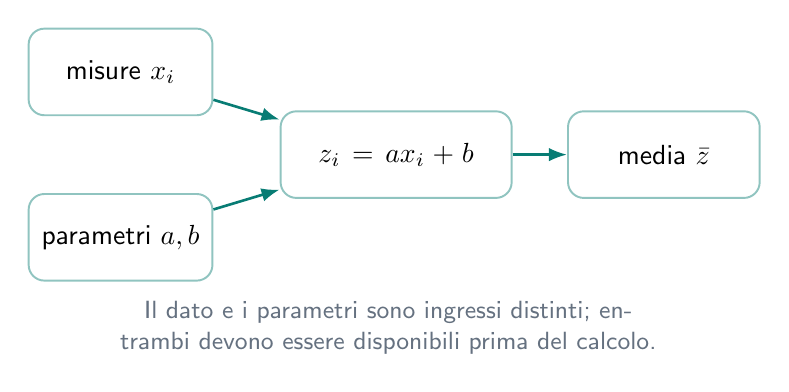
\begin{tikzpicture}[x=1cm,y=1cm]
\node[pFlow,text width=2.1cm] (d) at(1.3,3.1){misure $x_i$};
\node[pFlow,text width=2.1cm] (p) at(1.3,1){parametri $a,b$};
\node[pFlow,text width=2.7cm] (z) at(4.8,2.05){$z_i=ax_i+b$};
\node[pFlow,text width=2.2cm] (m) at(8.2,2.05){media $\bar z$};
\draw[pEdge](d)--(z);\draw[pEdge](p)--(z);\draw[pEdge](z)--(m);
\node[pNote,text width=8.7cm] at(4.7,-.15){Il dato e i parametri sono ingressi distinti; entrambi devono essere disponibili prima del calcolo.};
\end{tikzpicture}
\PBody{Per valori finiti, la linearità della media dà}
\[\bar z=a\bar x+b.\]
\PSmall{$a$ è il fattore di scala; $b$ la traslazione, nella stessa unità di $z$. Il caso numerico è adimensionale.}

\end{minipage}% 
\end{lrbox}
\typeout{FULLBOX:006:L:\the\ht\PilotLeftBox:\the\dp\PilotLeftBox}
\begin{lrbox}{\PilotRightBox}%
\begin{minipage}[t]{7.55cm}\raggedright\color{Ink}\fontsize{11.3}{14.8}\selectfont

\PCode{R · dichiarare e calcolare}{06_procedura.R}
\PBody{Lo script esplicita da dove provengono i numeri. Il risultato si ricostruisce a partire dagli ingressi.}
\PInfo{Qui $a$ e $b$ sono scelti. Una calibrazione strumentale stimerebbe i coefficienti da misure di riferimento e ne valuterebbe l'incertezza.}

\end{minipage}% 
\end{lrbox}
\typeout{FULLBOX:006:R:\the\ht\PilotRightBox:\the\dp\PilotRightBox}
\begin{frame}[plain]\hypertarget{slide6}{}
\bookmark[level=1,page=6]{Istruzioni nell’ordine delle dipendenze}
\begin{tikzpicture}[remember picture,overlay]
\PilotChrome{Istruzioni nell’ordine delle dipendenze}{PROGETTO E RIPRODUCIBILITÀ}{6}{I parametri usati in una trasformazione appartengono alla descrizione del risultato.}
\node[anchor=north west,inner sep=0] at ([xshift=0.96cm,yshift=-2.13cm]current page.north west) {\usebox{\PilotLeftBox}};
\node[anchor=north west,inner sep=0] at ([xshift=11.52cm,yshift=-2.13cm]current page.north west) {\usebox{\PilotRightBox}};

\end{tikzpicture}\end{frame}

% SLIDE 007 | Percorsi e controlli all’ingresso
\begin{lrbox}{\PilotLeftBox}%
\begin{minipage}[t]{10.05cm}\raggedright\color{Ink}\fontsize{11.3}{14.8}\selectfont

\PLabel{Il file atteso e la tabella letta}
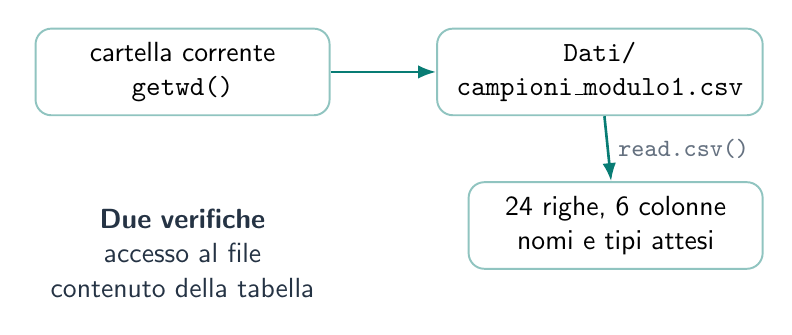
\begin{tikzpicture}[x=1cm,y=1cm]
\node[pFlow,text width=3.5cm] (p) at(2,3.2){cartella corrente\\\texttt{getwd()}};
\node[pFlow,text width=3.9cm] (f) at(7.3,3.2){\texttt{Dati/}\\\texttt{campioni\_modulo1.csv}};
\draw[pEdge](p)--(f);
\node[pFlow,text width=3.5cm] (t) at(7.5,1.25){24 righe, 6 colonne\\nomi e tipi attesi};
\draw[pEdge](f)--node[right,pNote]{\texttt{read.csv()}}(t);
\node[pLabel,text width=3.7cm] at(2,.9){\textbf{Due verifiche}\\accesso al file\\contenuto della tabella};
\end{tikzpicture}
\PBody{Un file trovato può contenere colonne o convenzioni inattese. La presenza sul disco e la correttezza dell'importazione richiedono controlli distinti.}
\PInfo{Le 24 righe sono una proprietà di questo file didattico. Ogni controllo deve derivare dalla specifica dei dati attesi.}

\end{minipage}% 
\end{lrbox}
\typeout{FULLBOX:007:L:\the\ht\PilotLeftBox:\the\dp\PilotLeftBox}
\begin{lrbox}{\PilotRightBox}%
\begin{minipage}[t]{7.55cm}\raggedright\color{Ink}\fontsize{11.3}{14.8}\selectfont

\PCode{R · interrompere un ingresso inatteso}{07_percorsi.R}
\PSmall{\texttt{file.path()} costruisce un percorso. \texttt{file.exists()} restituisce un valore logico; \texttt{stopifnot()} interrompe lo script se la condizione non è vera.}

\end{minipage}% 
\end{lrbox}
\typeout{FULLBOX:007:R:\the\ht\PilotRightBox:\the\dp\PilotRightBox}
\begin{frame}[plain]\hypertarget{slide7}{}
\bookmark[level=1,page=7]{Percorsi e controlli all’ingresso}
\begin{tikzpicture}[remember picture,overlay]
\PilotChrome{Percorsi e controlli all’ingresso}{PROGETTO E RIPRODUCIBILITÀ}{7}{Verificare accesso, nomi, tipi e numerosità prima di usare le colonne in un calcolo.}
\node[anchor=north west,inner sep=0] at ([xshift=0.96cm,yshift=-2.13cm]current page.north west) {\usebox{\PilotLeftBox}};
\node[anchor=north west,inner sep=0] at ([xshift=11.52cm,yshift=-2.13cm]current page.north west) {\usebox{\PilotRightBox}};

\end{tikzpicture}\end{frame}

% SLIDE 008 | Tellus: parametri e ricalcolo
\begin{lrbox}{\PilotLeftBox}%
\begin{minipage}[t]{10.05cm}\raggedright\color{Ink}\fontsize{11.3}{14.8}\selectfont

\PLabel{Oggetti espliciti e stato dell'analisi}
\PBody{Nel laboratorio \texttt{m02-progetto}, $x=1,\ldots,10$. Modificare pendenza e intercetta e confrontare la media prevista con quella mostrata.}
\vspace{3mm}
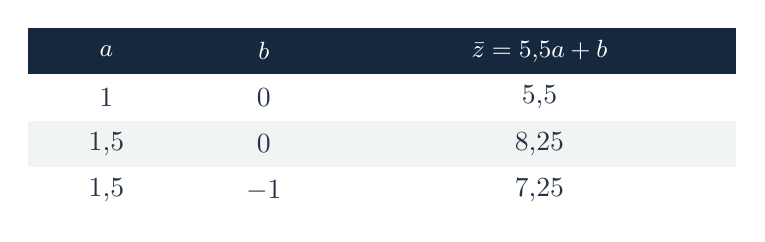
\begin{tikzpicture}[x=1cm,y=1cm]
\fill[Navy] (0,0) rectangle (9,0.59);
\node[font=\bfseries\fontsize{9.2}{11}\selectfont,text=white] at (1.0,0.295) {$a$};
\node[font=\bfseries\fontsize{9.2}{11}\selectfont,text=white] at (3.0,0.295) {$b$};
\node[font=\bfseries\fontsize{9.2}{11}\selectfont,text=white] at (6.5,0.295) {$\bar z=5{,}5a+b$};
\fill[white] (0,-0.59) rectangle (9,0.0);
\node[font=\fontsize{9.6}{12}\selectfont,text=Ink] at (1.0,-0.295) {1};
\node[font=\fontsize{9.6}{12}\selectfont,text=Ink] at (3.0,-0.295) {0};
\node[font=\fontsize{9.6}{12}\selectfont,text=Ink] at (6.5,-0.295) {5,5};
\fill[GeoTint] (0,-1.18) rectangle (9,-0.59);
\node[font=\fontsize{9.6}{12}\selectfont,text=Ink] at (1.0,-0.885) {1,5};
\node[font=\fontsize{9.6}{12}\selectfont,text=Ink] at (3.0,-0.885) {0};
\node[font=\fontsize{9.6}{12}\selectfont,text=Ink] at (6.5,-0.885) {8,25};
\fill[white] (0,-1.77) rectangle (9,-1.1800000000000002);
\node[font=\fontsize{9.6}{12}\selectfont,text=Ink] at (1.0,-1.475) {1,5};
\node[font=\fontsize{9.6}{12}\selectfont,text=Ink] at (3.0,-1.475) {$-1$};
\node[font=\fontsize{9.6}{12}\selectfont,text=Ink] at (6.5,-1.475) {7,25};
\end{tikzpicture}
\vspace{3mm}\PBody{Prima di eseguire, indicare quali risultati devono cambiare e quali ingressi rimangono fissati.}

\end{minipage}% 
\end{lrbox}
\typeout{FULLBOX:008:L:\the\ht\PilotLeftBox:\the\dp\PilotLeftBox}
\begin{lrbox}{\PilotRightBox}%
\begin{minipage}[t]{7.55cm}\raggedright\color{Ink}\fontsize{11.3}{14.8}\selectfont

\PLabel{Consegna}
\PBody{Riportare i tre scenari, la formula usata e la media restituita. Spiegare perché il risultato deve essere ricalcolato quando cambia un coefficiente.}
\vspace{3mm}\PInfo{Il vettore è prefissato: in questa attività il seme casuale non cambia il risultato. Il modello è deterministico.}
\vspace{4mm}\PBody{\href{https://marzione00.github.io/Lab_Geo/\#laboratorio/m02-progetto}{Apri l'esperimento M02 · Progetto}}
\PSmall{Il pannello consente $0{,}5\le a\le2$ e $-3\le b\le3$. I coefficienti sono scelti, senza una stima da standard.}

\end{minipage}% 
\end{lrbox}
\typeout{FULLBOX:008:R:\the\ht\PilotRightBox:\the\dp\PilotRightBox}
\begin{frame}[plain]\hypertarget{slide8}{}
\bookmark[level=1,page=8]{Tellus: parametri e ricalcolo}
\begin{tikzpicture}[remember picture,overlay]
\PilotChrome{Tellus: parametri e ricalcolo}{LABORATORIO · PROGETTO}{8}{Riproducibilità significa dichiarare dati, parametri e ordine dei calcoli, anche quando non compare alcuna simulazione.}
\node[anchor=north west,inner sep=0] at ([xshift=0.96cm,yshift=-2.13cm]current page.north west) {\usebox{\PilotLeftBox}};
\node[anchor=north west,inner sep=0] at ([xshift=11.52cm,yshift=-2.13cm]current page.north west) {\usebox{\PilotRightBox}};

\end{tikzpicture}\end{frame}

% SLIDE 009 | Tipi dei vettori e conversione implicita
\begin{lrbox}{\PilotLeftBox}%
\begin{minipage}[t]{10.05cm}\raggedright\color{Ink}\fontsize{11.3}{14.8}\selectfont

\PLabel{Gli elementi di un vettore atomico hanno un tipo comune}
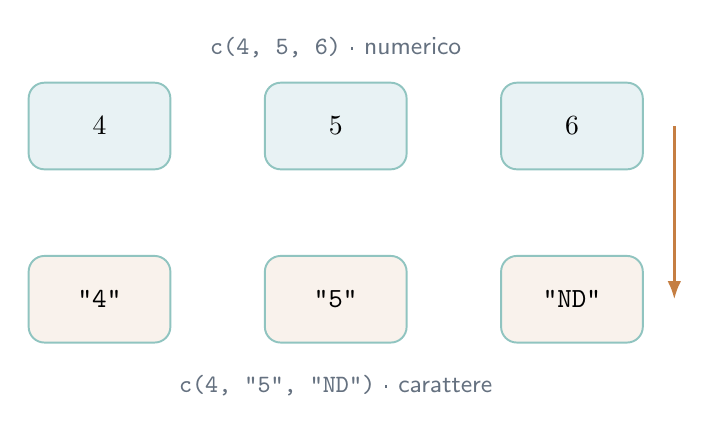
\begin{tikzpicture}[x=1cm,y=1cm]
\foreach \xx/\val in {1.4/4,4.4/5,7.4/6}{\node[pFlow,minimum width=1.8cm,fill=GeoA!10] at(\xx,3.0){$\val$};}
\node[pNote] at(4.4,4.0){\texttt{c(4, 5, 6)} · numerico};
\foreach \xx/\val in {1.4/4,4.4/5,7.4/ND}{\node[pFlow,minimum width=1.8cm,fill=GeoB!10] at(\xx,.8){\texttt{"\val"}};}
\node[pNote] at(4.4,-.3){\texttt{c(4, "5", "ND")} · carattere};
\draw[pEdge,GeoB](8.7,3)--(8.7,.8);
\end{tikzpicture}
\PBody{La presenza di testo induce una conversione al tipo carattere. La scrittura \texttt{"5"} conserva una stringa: il calcolo aritmetico richiede una conversione esplicita.}

\end{minipage}% 
\end{lrbox}
\typeout{FULLBOX:009:L:\the\ht\PilotLeftBox:\the\dp\PilotLeftBox}
\begin{lrbox}{\PilotRightBox}%
\begin{minipage}[t]{7.55cm}\raggedright\color{Ink}\fontsize{11.3}{14.8}\selectfont

\PCode{R · controllare il tipo}{09_tipi.R}
\PBody{\texttt{typeof()} descrive il tipo interno. \texttt{is.numeric()} verifica se l'oggetto è numerico.}
\PInfo{Un identificativo può essere formato da cifre e restare testo. Convertire \texttt{"007"} in numero elimina gli zeri iniziali, che possono appartenere al codice.}

\end{minipage}% 
\end{lrbox}
\typeout{FULLBOX:009:R:\the\ht\PilotRightBox:\the\dp\PilotRightBox}
\begin{frame}[plain]\hypertarget{slide9}{}
\bookmark[level=1,page=9]{Tipi dei vettori e conversione implicita}
\begin{tikzpicture}[remember picture,overlay]
\PilotChrome{Tipi dei vettori e conversione implicita}{VETTORI E SELEZIONI}{9}{Il tipo di memorizzazione determina le operazioni possibili; il significato della variabile stabilisce quelle appropriate.}
\node[anchor=north west,inner sep=0] at ([xshift=0.96cm,yshift=-2.13cm]current page.north west) {\usebox{\PilotLeftBox}};
\node[anchor=north west,inner sep=0] at ([xshift=11.52cm,yshift=-2.13cm]current page.north west) {\usebox{\PilotRightBox}};

\end{tikzpicture}\end{frame}

% SLIDE 010 | Indici di righe e colonne
\begin{lrbox}{\PilotLeftBox}%
\begin{minipage}[t]{10.05cm}\raggedright\color{Ink}\fontsize{11.3}{14.8}\selectfont

\PLabel{Due coordinate per una tabella}
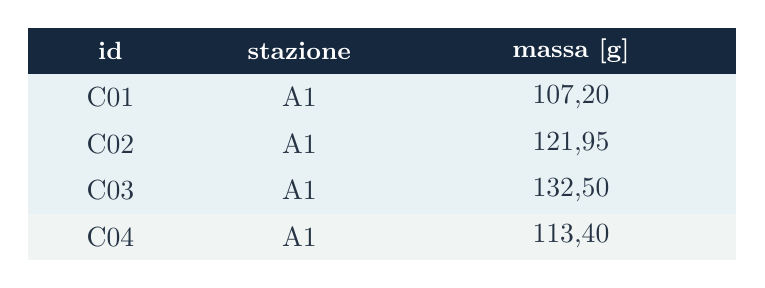
\begin{tikzpicture}[x=1cm,y=1cm]
\fill[Navy] (0,0) rectangle (9.0,0.59);
\node[font=\bfseries\fontsize{9.2}{11}\selectfont,text=white] at (1.05,0.295) {id};
\node[font=\bfseries\fontsize{9.2}{11}\selectfont,text=white] at (3.45,0.295) {stazione};
\node[font=\bfseries\fontsize{9.2}{11}\selectfont,text=white] at (6.9,0.295) {massa [g]};
\fill[GeoA!10] (0,-0.59) rectangle (9.0,0.0);
\node[font=\fontsize{9.6}{12}\selectfont,text=Ink] at (1.05,-0.295) {C01};
\node[font=\fontsize{9.6}{12}\selectfont,text=Ink] at (3.45,-0.295) {A1};
\node[font=\fontsize{9.6}{12}\selectfont,text=Ink] at (6.9,-0.295) {107,20};
\fill[GeoA!10] (0,-1.18) rectangle (9.0,-0.59);
\node[font=\fontsize{9.6}{12}\selectfont,text=Ink] at (1.05,-0.885) {C02};
\node[font=\fontsize{9.6}{12}\selectfont,text=Ink] at (3.45,-0.885) {A1};
\node[font=\fontsize{9.6}{12}\selectfont,text=Ink] at (6.9,-0.885) {121,95};
\fill[GeoA!10] (0,-1.77) rectangle (9.0,-1.1800000000000002);
\node[font=\fontsize{9.6}{12}\selectfont,text=Ink] at (1.05,-1.475) {C03};
\node[font=\fontsize{9.6}{12}\selectfont,text=Ink] at (3.45,-1.475) {A1};
\node[font=\fontsize{9.6}{12}\selectfont,text=Ink] at (6.9,-1.475) {132,50};
\fill[GeoTint] (0,-2.36) rectangle (9.0,-1.77);
\node[font=\fontsize{9.6}{12}\selectfont,text=Ink] at (1.05,-2.065) {C04};
\node[font=\fontsize{9.6}{12}\selectfont,text=Ink] at (3.45,-2.065) {A1};
\node[font=\fontsize{9.6}{12}\selectfont,text=Ink] at (6.9,-2.065) {113,40};
\end{tikzpicture}
\vspace{4mm}
\[\texttt{campioni[righe, colonne]}\]
\PBody{Prima della virgola si indicano le righe; dopo la virgola, le colonne. Lasciare una delle due posizioni vuota conserva tutte le righe o tutte le colonne.}
\PSmall{La porzione mostrata proviene dalle prime quattro righe del CSV dei provini. Le masse sono in grammi.}

\end{minipage}% 
\end{lrbox}
\typeout{FULLBOX:010:L:\the\ht\PilotLeftBox:\the\dp\PilotLeftBox}
\begin{lrbox}{\PilotRightBox}%
\begin{minipage}[t]{7.55cm}\raggedright\color{Ink}\fontsize{11.3}{14.8}\selectfont

\PCode{R · scegliere posizioni e nomi}{10_posizioni.R}
\PSmall{Gli indici partono da 1. \texttt{c(1,3)} combina due posizioni. Con una tabella, \texttt{["massa\_g"]} conserva la struttura tabellare; \texttt{\$massa\_g} estrae il vettore.}

\end{minipage}% 
\end{lrbox}
\typeout{FULLBOX:010:R:\the\ht\PilotRightBox:\the\dp\PilotRightBox}
\begin{frame}[plain]\hypertarget{slide10}{}
\bookmark[level=1,page=10]{Indici di righe e colonne}
\begin{tikzpicture}[remember picture,overlay]
\PilotChrome{Indici di righe e colonne}{VETTORI E SELEZIONI}{10}{La posizione di una misura ha significato finché rimane collegata all’identificativo della stessa unità.}
\node[anchor=north west,inner sep=0] at ([xshift=0.96cm,yshift=-2.13cm]current page.north west) {\usebox{\PilotLeftBox}};
\node[anchor=north west,inner sep=0] at ([xshift=11.52cm,yshift=-2.13cm]current page.north west) {\usebox{\PilotRightBox}};

\end{tikzpicture}\end{frame}

% SLIDE 011 | Selezionare e ordinare righe intere
\begin{lrbox}{\PilotLeftBox}%
\begin{minipage}[t]{10.05cm}\raggedright\color{Ink}\fontsize{11.3}{14.8}\selectfont

\PLabel{L'identificativo accompagna tutte le misure}
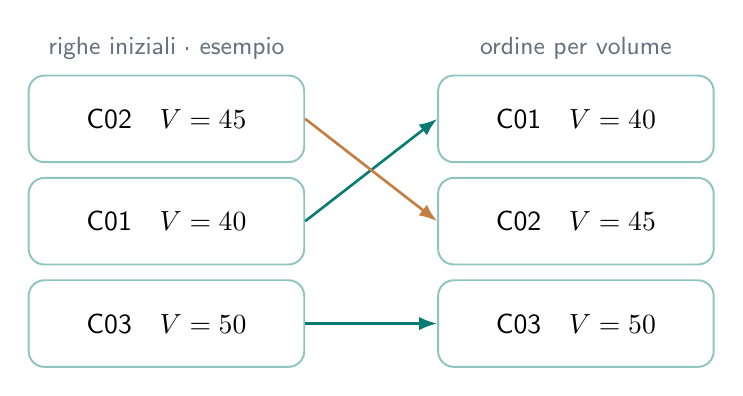
\begin{tikzpicture}[x=1cm,y=1cm]
\node[pNote] at(2.1,3.8){righe iniziali · esempio};
\node[pNote] at(7.3,3.8){ordine per volume};
\foreach \yy/\id/\v in {2.9/C02/45,1.6/C01/40,.3/C03/50}{
 \node[pFlow,minimum width=3.5cm] (l\id) at(2.1,\yy){\id\quad $V=\v$};}
\foreach \yy/\id/\v in {2.9/C01/40,1.6/C02/45,.3/C03/50}{
 \node[pFlow,minimum width=3.5cm] (r\id) at(7.3,\yy){\id\quad $V=\v$};}
\draw[pEdge] (lC01.east)--(rC01.west);\draw[pEdge,GeoB] (lC02.east)--(rC02.west);\draw[pEdge] (lC03.east)--(rC03.west);
\end{tikzpicture}
\PBody{Ordinare soltanto i valori di una colonna rompe le coppie fra misure dello stesso provino. \texttt{order()} restituisce una permutazione da applicare all'intera tabella.}
\PSmall{Volumi in cm$^3$. Il piccolo esempio mostra tre provini del CSV in un ordine illustrativo.}

\end{minipage}% 
\end{lrbox}
\typeout{FULLBOX:011:L:\the\ht\PilotLeftBox:\the\dp\PilotLeftBox}
\begin{lrbox}{\PilotRightBox}%
\begin{minipage}[t]{7.55cm}\raggedright\color{Ink}\fontsize{11.3}{14.8}\selectfont

\PCode{R · filtrare e ordinare}{11_selezione.R}
\PSmall{\texttt{==} confronta; \texttt{<-} assegna. \texttt{sel} contiene un valore logico per riga. \texttt{[sel, ]} conserva tutte le colonne.}
\PInfo{Conservare il criterio di inclusione insieme al numero di righe selezionate.}

\end{minipage}% 
\end{lrbox}
\typeout{FULLBOX:011:R:\the\ht\PilotRightBox:\the\dp\PilotRightBox}
\begin{frame}[plain]\hypertarget{slide11}{}
\bookmark[level=1,page=11]{Selezionare e ordinare righe intere}
\begin{tikzpicture}[remember picture,overlay]
\PilotChrome{Selezionare e ordinare righe intere}{VETTORI E SELEZIONI}{11}{Filtri e ordinamenti vanno applicati alla tabella intera per conservare l’associazione fra identificativi e misure.}
\node[anchor=north west,inner sep=0] at ([xshift=0.96cm,yshift=-2.13cm]current page.north west) {\usebox{\PilotLeftBox}};
\node[anchor=north west,inner sep=0] at ([xshift=11.52cm,yshift=-2.13cm]current page.north west) {\usebox{\PilotRightBox}};

\end{tikzpicture}\end{frame}

% SLIDE 012 | Condizioni logiche e sottoinsiemi
\begin{lrbox}{\PilotLeftBox}%
\begin{minipage}[t]{10.05cm}\raggedright\color{Ink}\fontsize{11.3}{14.8}\selectfont

\PLabel{Appartenenza all'affioramento e volume minimo}
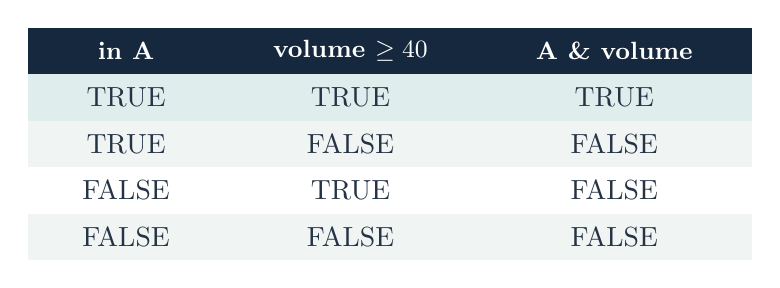
\begin{tikzpicture}[x=1cm,y=1cm]
\fill[Navy] (0,0) rectangle (9.2,0.59);
\node[font=\bfseries\fontsize{9.2}{11}\selectfont,text=white] at (1.25,0.295) {in A};
\node[font=\bfseries\fontsize{9.2}{11}\selectfont,text=white] at (4.1,0.295) {volume $\ge40$};
\node[font=\bfseries\fontsize{9.2}{11}\selectfont,text=white] at (7.45,0.295) {A \& volume};
\fill[Classical!13] (0,-0.59) rectangle (9.2,0.0);
\node[font=\fontsize{9.6}{12}\selectfont,text=Ink] at (1.25,-0.295) {TRUE};
\node[font=\fontsize{9.6}{12}\selectfont,text=Ink] at (4.1,-0.295) {TRUE};
\node[font=\fontsize{9.6}{12}\selectfont,text=Ink] at (7.45,-0.295) {TRUE};
\fill[GeoTint] (0,-1.18) rectangle (9.2,-0.59);
\node[font=\fontsize{9.6}{12}\selectfont,text=Ink] at (1.25,-0.885) {TRUE};
\node[font=\fontsize{9.6}{12}\selectfont,text=Ink] at (4.1,-0.885) {FALSE};
\node[font=\fontsize{9.6}{12}\selectfont,text=Ink] at (7.45,-0.885) {FALSE};
\fill[white] (0,-1.77) rectangle (9.2,-1.1800000000000002);
\node[font=\fontsize{9.6}{12}\selectfont,text=Ink] at (1.25,-1.475) {FALSE};
\node[font=\fontsize{9.6}{12}\selectfont,text=Ink] at (4.1,-1.475) {TRUE};
\node[font=\fontsize{9.6}{12}\selectfont,text=Ink] at (7.45,-1.475) {FALSE};
\fill[GeoTint] (0,-2.36) rectangle (9.2,-1.77);
\node[font=\fontsize{9.6}{12}\selectfont,text=Ink] at (1.25,-2.065) {FALSE};
\node[font=\fontsize{9.6}{12}\selectfont,text=Ink] at (4.1,-2.065) {FALSE};
\node[font=\fontsize{9.6}{12}\selectfont,text=Ink] at (7.45,-2.065) {FALSE};
\end{tikzpicture}
\vspace{3mm}
\[\mathcal S=\{i:A_i=\mathrm A\ \land\ V_i\ge40\}.\]
\PSmall{$i$ identifica il provino; $A_i$ l'affioramento; $V_i$ il volume in cm$^3$. La soglia 40 è una scelta dell'esempio.}
\PBody{\texttt{\&} richiede entrambe le condizioni; \texttt{|} ne richiede almeno una; \texttt{!} nega un valore logico.}

\end{minipage}% 
\end{lrbox}
\typeout{FULLBOX:012:L:\the\ht\PilotLeftBox:\the\dp\PilotLeftBox}
\begin{lrbox}{\PilotRightBox}%
\begin{minipage}[t]{7.55cm}\raggedright\color{Ink}\fontsize{11.3}{14.8}\selectfont

\PCode{R · combinare condizioni}{12_logica.R}
\PSmall{\texttt{\%in\%} verifica l'appartenenza a un insieme di valori ammessi. \texttt{sum(sel)} conta i \texttt{TRUE} quando la maschera non contiene \texttt{NA}.}
\PInfo{Per confrontare riga per riga usare \texttt{\&} e \texttt{|}. Gli operatori \texttt{\&\&} e \texttt{||} servono al controllo di flusso su condizioni singole.}

\end{minipage}% 
\end{lrbox}
\typeout{FULLBOX:012:R:\the\ht\PilotRightBox:\the\dp\PilotRightBox}
\begin{frame}[plain]\hypertarget{slide12}{}
\bookmark[level=1,page=12]{Condizioni logiche e sottoinsiemi}
\begin{tikzpicture}[remember picture,overlay]
\PilotChrome{Condizioni logiche e sottoinsiemi}{VETTORI E SELEZIONI}{12}{Scrivere esplicitamente intersezioni, unioni ed estremi delle condizioni che definiscono il campione analitico.}
\node[anchor=north west,inner sep=0] at ([xshift=0.96cm,yshift=-2.13cm]current page.north west) {\usebox{\PilotLeftBox}};
\node[anchor=north west,inner sep=0] at ([xshift=11.52cm,yshift=-2.13cm]current page.north west) {\usebox{\PilotRightBox}};

\end{tikzpicture}\end{frame}

% SLIDE 013 | Valori mancanti nelle condizioni logiche
\begin{lrbox}{\PilotLeftBox}%
\begin{minipage}[t]{10.05cm}\raggedright\color{Ink}\fontsize{11.3}{14.8}\selectfont

\PLabel{Un confronto con NA non identifica un valore}
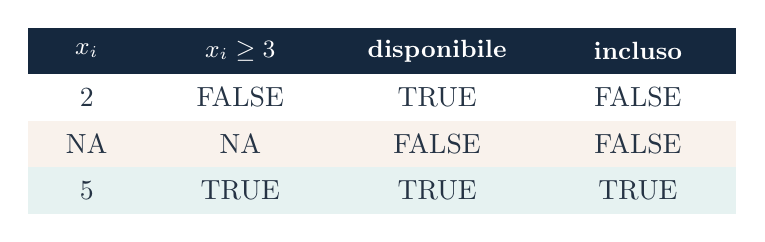
\begin{tikzpicture}[x=1cm,y=1cm]
\fill[Navy] (0,0) rectangle (9.0,0.59);
\node[font=\bfseries\fontsize{9.2}{11}\selectfont,text=white] at (0.75,0.295) {$x_i$};
\node[font=\bfseries\fontsize{9.2}{11}\selectfont,text=white] at (2.7,0.295) {$x_i\ge3$};
\node[font=\bfseries\fontsize{9.2}{11}\selectfont,text=white] at (5.2,0.295) {disponibile};
\node[font=\bfseries\fontsize{9.2}{11}\selectfont,text=white] at (7.75,0.295) {incluso};
\fill[white] (0,-0.59) rectangle (9.0,0.0);
\node[font=\fontsize{9.6}{12}\selectfont,text=Ink] at (0.75,-0.295) {2};
\node[font=\fontsize{9.6}{12}\selectfont,text=Ink] at (2.7,-0.295) {FALSE};
\node[font=\fontsize{9.6}{12}\selectfont,text=Ink] at (5.2,-0.295) {TRUE};
\node[font=\fontsize{9.6}{12}\selectfont,text=Ink] at (7.75,-0.295) {FALSE};
\fill[GeoB!10] (0,-1.18) rectangle (9.0,-0.59);
\node[font=\fontsize{9.6}{12}\selectfont,text=Ink] at (0.75,-0.885) {NA};
\node[font=\fontsize{9.6}{12}\selectfont,text=Ink] at (2.7,-0.885) {NA};
\node[font=\fontsize{9.6}{12}\selectfont,text=Ink] at (5.2,-0.885) {FALSE};
\node[font=\fontsize{9.6}{12}\selectfont,text=Ink] at (7.75,-0.885) {FALSE};
\fill[Classical!10] (0,-1.77) rectangle (9.0,-1.1800000000000002);
\node[font=\fontsize{9.6}{12}\selectfont,text=Ink] at (0.75,-1.475) {5};
\node[font=\fontsize{9.6}{12}\selectfont,text=Ink] at (2.7,-1.475) {TRUE};
\node[font=\fontsize{9.6}{12}\selectfont,text=Ink] at (5.2,-1.475) {TRUE};
\node[font=\fontsize{9.6}{12}\selectfont,text=Ink] at (7.75,-1.475) {TRUE};
\end{tikzpicture}
\vspace{4mm}\PBody{\texttt{NA} indica informazione mancante. Se la selezione deve includere soltanto misure disponibili, occorre scrivere questa condizione nel filtro.}
\PInfo{Un indice logico con \texttt{NA} può produrre elementi o righe interamente mancanti nella selezione. Controllare la maschera prima di usarla.}

\end{minipage}% 
\end{lrbox}
\typeout{FULLBOX:013:L:\the\ht\PilotLeftBox:\the\dp\PilotLeftBox}
\begin{lrbox}{\PilotRightBox}%
\begin{minipage}[t]{7.55cm}\raggedright\color{Ink}\fontsize{11.3}{14.8}\selectfont

\PCode{R · un filtro con esito definito}{13_na_logici.R}
\PSmall{\texttt{is.na()} riconosce i mancanti; \texttt{anyNA()} verifica se ne esiste almeno uno. Il simbolo \texttt{!} inverte \texttt{TRUE} e \texttt{FALSE}.}
\vspace{2mm}\PSmall{La regola esclude l'osservazione assente da questo calcolo. Il valore originale resta conservato: l'esclusione non ne spiega la causa.}

\end{minipage}% 
\end{lrbox}
\typeout{FULLBOX:013:R:\the\ht\PilotRightBox:\the\dp\PilotRightBox}
\begin{frame}[plain]\hypertarget{slide13}{}
\bookmark[level=1,page=13]{Valori mancanti nelle condizioni logiche}
\begin{tikzpicture}[remember picture,overlay]
\PilotChrome{Valori mancanti nelle condizioni logiche}{VETTORI E SELEZIONI}{13}{Una maschera di selezione deve avere un esito definito per ogni riga, con una regola dichiarata per i mancanti.}
\node[anchor=north west,inner sep=0] at ([xshift=0.96cm,yshift=-2.13cm]current page.north west) {\usebox{\PilotLeftBox}};
\node[anchor=north west,inner sep=0] at ([xshift=11.52cm,yshift=-2.13cm]current page.north west) {\usebox{\PilotRightBox}};

\end{tikzpicture}\end{frame}

% SLIDE 014 | Categorie ordinate e date
\begin{lrbox}{\PilotLeftBox}%
\begin{minipage}[t]{10.05cm}\raggedright\color{Ink}\fontsize{11.3}{14.8}\selectfont

\PLabel{Due ordinamenti con significati diversi}
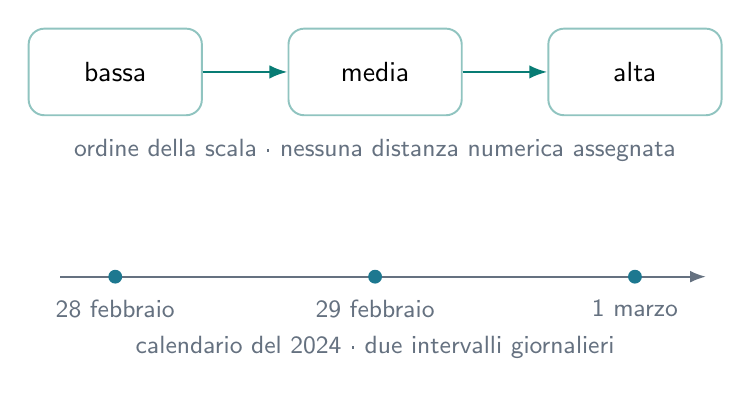
\begin{tikzpicture}[x=1cm,y=1cm]
\node[pFlow,minimum width=2.2cm] (a) at(1.4,3.3){bassa};
\node[pFlow,minimum width=2.2cm] (b) at(4.7,3.3){media};
\node[pFlow,minimum width=2.2cm] (c) at(8,3.3){alta};
\draw[pEdge](a)--(b);\draw[pEdge](b)--(c);
\node[pNote] at(4.7,2.3){ordine della scala · nessuna distanza numerica assegnata};
\draw[pAxis](.7,.7)--(8.9,.7);
\foreach \xx/\lbl in {1.4/28 febbraio,4.7/29 febbraio,8/1 marzo}{\fill[GeoA](\xx,.7)circle(2.5pt);\node[pNote,below=5pt] at(\xx,.7){\lbl};}
\node[pNote] at(4.7,-.2){calendario del 2024 · due intervalli giornalieri};
\end{tikzpicture}
\PBody{I livelli di un fattore descrivono categorie ammesse. Una data memorizzata come \texttt{Date} permette ordinamenti e differenze secondo il calendario.}

\end{minipage}% 
\end{lrbox}
\typeout{FULLBOX:014:L:\the\ht\PilotLeftBox:\the\dp\PilotLeftBox}
\begin{lrbox}{\PilotRightBox}%
\begin{minipage}[t]{7.55cm}\raggedright\color{Ink}\fontsize{11.3}{14.8}\selectfont

\PCode{R · dichiarare livello e calendario}{14_categorie_date.R}
\PSmall{\texttt{ordered=TRUE} dichiara l'ordine dei livelli. \texttt{as.Date()} legge qui anno-mese-giorno; \texttt{diff()} calcola la differenza fra date successive.}

\end{minipage}% 
\end{lrbox}
\typeout{FULLBOX:014:R:\the\ht\PilotRightBox:\the\dp\PilotRightBox}
\begin{frame}[plain]\hypertarget{slide14}{}
\bookmark[level=1,page=14]{Categorie ordinate e date}
\begin{tikzpicture}[remember picture,overlay]
\PilotChrome{Categorie ordinate e date}{VETTORI E SELEZIONI}{14}{L’ordine delle categorie deve derivare dalla scala di misura; quello delle date dalla convenzione di calendario dichiarata.}
\node[anchor=north west,inner sep=0] at ([xshift=0.96cm,yshift=-2.13cm]current page.north west) {\usebox{\PilotLeftBox}};
\node[anchor=north west,inner sep=0] at ([xshift=11.52cm,yshift=-2.13cm]current page.north west) {\usebox{\PilotRightBox}};

\end{tikzpicture}\end{frame}

% SLIDE 015 | Tellus: estremi inclusi ed esclusi
\begin{lrbox}{\PilotLeftBox}%
\begin{minipage}[t]{10.05cm}\raggedright\color{Ink}\fontsize{11.3}{14.8}\selectfont

\PLabel{Intervallo chiuso sulla griglia del sito}
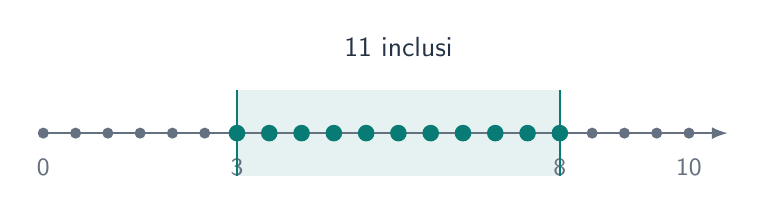
\begin{tikzpicture}[x=.82cm,y=1cm]
\fill[Classical!10](3,.35)rectangle(8,1.45);
\draw[pAxis](0,.9)--(10.6,.9);
\foreach \x in {0,.5,...,10}{\fill[Muted](\x,.9)circle(2pt);}
\foreach \x in {3,3.5,...,8}{\fill[Classical](\x,.9)circle(3pt);}
\foreach \x in {0,3,8,10}{\node[pNote,below=6pt] at(\x,.9){\x};}
\node[pLabel] at(5.5,2){11 inclusi};
\draw[Classical,line width=.9pt](3,.35)--(3,1.45);\draw[Classical,line width=.9pt](8,.35)--(8,1.45);
\end{tikzpicture}
\[I_i=\mathbf1(a\le x_i\le b),\quad n_{\rm inclusi}=\sum_i I_i.\]
\PSmall{$I_i$ vale 1 se la riga è inclusa, 0 altrimenti. La griglia contiene 21 valori, da 0 a 10 con passo 0,5.}
\PBody{Confrontare $[3,8]$, $[4,7]$ e gli estremi inseriti nell'ordine inverso. Prevedere i conteggi prima dell'esecuzione.}
\PSmall{Consegna: intervallo effettivo, inclusi, esclusi e una riga che cambierebbe stato usando una disuguaglianza stretta.}

\end{minipage}% 
\end{lrbox}
\typeout{FULLBOX:015:L:\the\ht\PilotLeftBox:\the\dp\PilotLeftBox}
\begin{lrbox}{\PilotRightBox}%
\begin{minipage}[t]{7.55cm}\raggedright\color{Ink}\fontsize{11.3}{14.8}\selectfont

\PCode{R · riprodurre il filtro}{15_lab_selezioni.R}
\PSmall{Il sito ordina i due estremi con \texttt{min()} e \texttt{max()}: invertirli conserva l'intervallo. Il criterio comprende gli estremi.}
\vspace{3mm}\PBody{\href{https://marzione00.github.io/Lab_Geo/\#laboratorio/m02-selezioni}{Apri l'esperimento M02 · Selezioni}}

\end{minipage}% 
\end{lrbox}
\typeout{FULLBOX:015:R:\the\ht\PilotRightBox:\the\dp\PilotRightBox}
\begin{frame}[plain]\hypertarget{slide15}{}
\bookmark[level=1,page=15]{Tellus: estremi inclusi ed esclusi}
\begin{tikzpicture}[remember picture,overlay]
\PilotChrome{Tellus: estremi inclusi ed esclusi}{LABORATORIO · SELEZIONI}{15}{La convenzione sugli estremi può cambiare il campione selezionato, soprattutto con misure discrete o arrotondate.}
\node[anchor=north west,inner sep=0] at ([xshift=0.96cm,yshift=-2.13cm]current page.north west) {\usebox{\PilotLeftBox}};
\node[anchor=north west,inner sep=0] at ([xshift=11.52cm,yshift=-2.13cm]current page.north west) {\usebox{\PilotRightBox}};

\end{tikzpicture}\end{frame}

% SLIDE 016 | Il CSV e le sue convenzioni
\begin{lrbox}{\PilotLeftBox}%
\begin{minipage}[t]{10.05cm}\raggedright\color{Ink}\fontsize{11.3}{14.8}\selectfont

\PLabel{Testo prima della tabella}
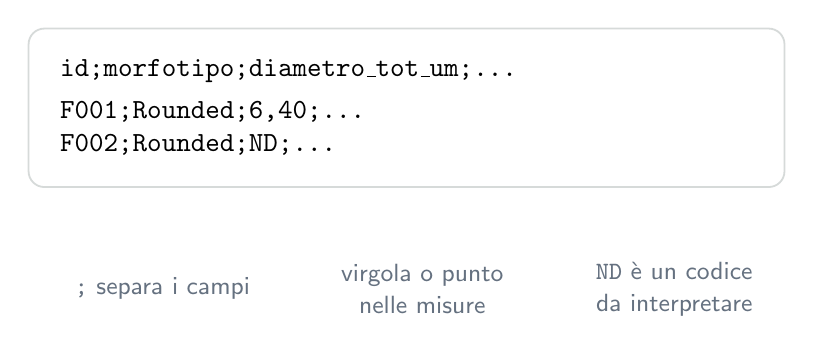
\begin{tikzpicture}[x=1cm,y=1cm]
\node[pGroup,text width=8.8cm,align=left,inner sep=4mm] at(4.6,2.5){\ttfamily\fontsize{10}{15}\selectfont id;morfotipo;diametro\_tot\_um;...\\F001;Rounded;6,40;...\\F002;Rounded;ND;...};
\node[pNote,text width=2.5cm] (s) at(1.5,.2){\texttt{;} separa i campi};
\node[pNote,text width=2.8cm] (d) at(4.8,.2){virgola o punto\\nelle misure};
\node[pNote,text width=2.6cm] (m) at(8,.2){\texttt{ND} è un codice\\da interpretare};
\end{tikzpicture}
\PBody{L'estensione \texttt{.csv} non stabilisce separatore di campo, simbolo decimale o significato dei codici speciali. Le convenzioni devono essere verificate sul file e sulla documentazione.}
\PSmall{Estratto abbreviato del file dei fossili. Il CSV contiene cinque colonne originali e 25 registrazioni.}

\end{minipage}% 
\end{lrbox}
\typeout{FULLBOX:016:L:\the\ht\PilotLeftBox:\the\dp\PilotLeftBox}
\begin{lrbox}{\PilotRightBox}%
\begin{minipage}[t]{7.55cm}\raggedright\color{Ink}\fontsize{11.3}{14.8}\selectfont

\PCode{R · leggere le prime righe}{16_file_testuale.R}
\PBody{\texttt{readLines()} mostra righe di testo. Permette di riconoscere intestazioni e delimitatori prima della lettura tabellare.}
\PInfo{Un file Excel richiede anche foglio, intervallo e riga di intestazione. Titoli, note e celle unite devono essere distinti dalle osservazioni.}
\PSmall{Gli esempi della lezione usano CSV locali, così le convenzioni sono visibili e il codice resta eseguibile con R di base.}

\end{minipage}% 
\end{lrbox}
\typeout{FULLBOX:016:R:\the\ht\PilotRightBox:\the\dp\PilotRightBox}
\begin{frame}[plain]\hypertarget{slide16}{}
\bookmark[level=1,page=16]{Il CSV e le sue convenzioni}
\begin{tikzpicture}[remember picture,overlay]
\PilotChrome{Il CSV e le sue convenzioni}{IMPORTAZIONE E CONVERSIONI}{16}{Documentare separatore, decimali, codifica del testo e codici dei mancanti insieme al file importato.}
\node[anchor=north west,inner sep=0] at ([xshift=0.96cm,yshift=-2.13cm]current page.north west) {\usebox{\PilotLeftBox}};
\node[anchor=north west,inner sep=0] at ([xshift=11.52cm,yshift=-2.13cm]current page.north west) {\usebox{\PilotRightBox}};

\end{tikzpicture}\end{frame}

% SLIDE 017 | Separatore di campo e simbolo decimale
\begin{lrbox}{\PilotLeftBox}%
\begin{minipage}[t]{10.05cm}\raggedright\color{Ink}\fontsize{11.3}{14.8}\selectfont

\PLabel{Due funzioni distinte nella stessa riga}
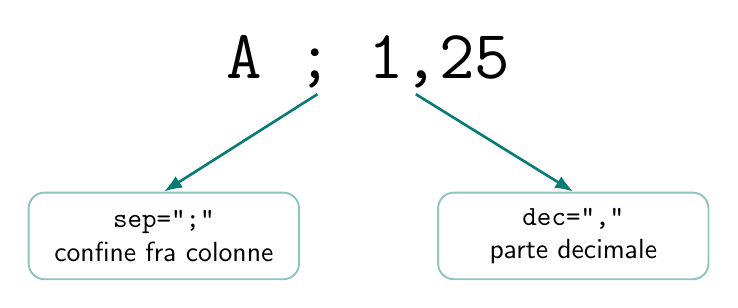
\begin{tikzpicture}[x=1cm,y=1cm]
\node[font=\ttfamily\fontsize{24}{28}\selectfont] at(4.6,3.3){A\ ;\ 1,25};
\node[pFlow,text width=3.2cm] (c) at(2,1.1){\texttt{sep=";"}\\confine fra colonne};
\node[pFlow,text width=3.2cm] (d) at(7.2,1.1){\texttt{dec=","}\\parte decimale};
\draw[pEdge](3.95,2.9)--(c.north);\draw[pEdge](5.2,2.9)--(d.north);
\end{tikzpicture}
\PBody{Le convenzioni standard di \texttt{read.csv()} sono virgola fra campi e punto decimale. \texttt{read.csv2()} usa punto e virgola fra campi e virgola decimale.}
\PInfo{Nel file dei fossili convivono il punto e la virgola come simboli decimali. Una prima lettura come testo conserva entrambe le scritture.}

\end{minipage}% 
\end{lrbox}
\typeout{FULLBOX:017:L:\the\ht\PilotLeftBox:\the\dp\PilotLeftBox}
\begin{lrbox}{\PilotRightBox}%
\begin{minipage}[t]{7.55cm}\raggedright\color{Ink}\fontsize{11.3}{14.8}\selectfont

\PCode{R · convenzioni dichiarate}{17_separatori.R}
\PSmall{Nella stringa, \texttt{\textbackslash n} indica una nuova riga. \texttt{text=csv} usa quel contenuto al posto di un file esterno.}
\vspace{3mm}\PBody{Dopo la lettura, verificare che \texttt{valore} sia numerico e che i numeri coincidano con quelli scritti nel testo.}
\PSmall{La media dell'esempio usa due numeri, 1,25 e 2,50. Una colonna contenente testo richiederebbe una diagnosi della conversione.}

\end{minipage}% 
\end{lrbox}
\typeout{FULLBOX:017:R:\the\ht\PilotRightBox:\the\dp\PilotRightBox}
\begin{frame}[plain]\hypertarget{slide17}{}
\bookmark[level=1,page=17]{Separatore di campo e simbolo decimale}
\begin{tikzpicture}[remember picture,overlay]
\PilotChrome{Separatore di campo e simbolo decimale}{IMPORTAZIONE E CONVERSIONI}{17}{Separatore di campo e simbolo decimale sono parametri differenti: entrambi devono corrispondere al formato di origine.}
\node[anchor=north west,inner sep=0] at ([xshift=0.96cm,yshift=-2.13cm]current page.north west) {\usebox{\PilotLeftBox}};
\node[anchor=north west,inner sep=0] at ([xshift=11.52cm,yshift=-2.13cm]current page.north west) {\usebox{\PilotRightBox}};

\end{tikzpicture}\end{frame}

% SLIDE 018 | Importazione conservativa del testo
\begin{lrbox}{\PilotLeftBox}%
\begin{minipage}[t]{10.05cm}\raggedright\color{Ink}\fontsize{11.3}{14.8}\selectfont

\PLabel{Una riga rintracciabile nel file di origine}
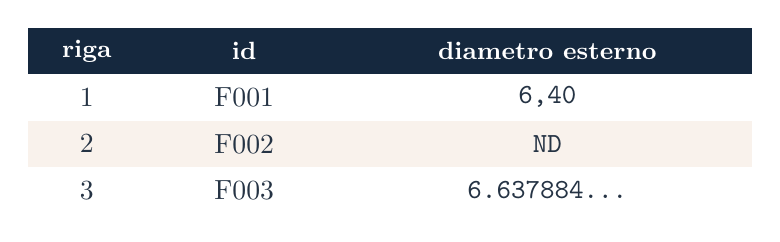
\begin{tikzpicture}[x=1cm,y=1cm]
\fill[Navy] (0,0) rectangle (9.2,0.59);
\node[font=\bfseries\fontsize{9.2}{11}\selectfont,text=white] at (0.75,0.295) {riga};
\node[font=\bfseries\fontsize{9.2}{11}\selectfont,text=white] at (2.75,0.295) {id};
\node[font=\bfseries\fontsize{9.2}{11}\selectfont,text=white] at (6.6,0.295) {diametro esterno};
\fill[white] (0,-0.59) rectangle (9.2,0.0);
\node[font=\fontsize{9.6}{12}\selectfont,text=Ink] at (0.75,-0.295) {1};
\node[font=\fontsize{9.6}{12}\selectfont,text=Ink] at (2.75,-0.295) {F001};
\node[font=\fontsize{9.6}{12}\selectfont,text=Ink] at (6.6,-0.295) {\texttt{6,40}};
\fill[GeoB!10] (0,-1.18) rectangle (9.2,-0.59);
\node[font=\fontsize{9.6}{12}\selectfont,text=Ink] at (0.75,-0.885) {2};
\node[font=\fontsize{9.6}{12}\selectfont,text=Ink] at (2.75,-0.885) {F002};
\node[font=\fontsize{9.6}{12}\selectfont,text=Ink] at (6.6,-0.885) {\texttt{ND}};
\fill[white] (0,-1.77) rectangle (9.2,-1.1800000000000002);
\node[font=\fontsize{9.6}{12}\selectfont,text=Ink] at (0.75,-1.475) {3};
\node[font=\fontsize{9.6}{12}\selectfont,text=Ink] at (2.75,-1.475) {F003};
\node[font=\fontsize{9.6}{12}\selectfont,text=Ink] at (6.6,-1.475) {\texttt{6.637884...}};
\end{tikzpicture}
\vspace{4mm}\PBody{\texttt{colClasses="character"} conserva le colonne come testo. \texttt{na.strings=character()} evita di sostituire codici testuali prima di averli interpretati.}
\PInfo{\texttt{riga\_origine} serve a ritrovare una registrazione anche se l'identificativo compare più volte. Va aggiunta prima di ordinamenti o filtri.}

\end{minipage}% 
\end{lrbox}
\typeout{FULLBOX:018:L:\the\ht\PilotLeftBox:\the\dp\PilotLeftBox}
\begin{lrbox}{\PilotRightBox}%
\begin{minipage}[t]{7.55cm}\raggedright\color{Ink}\fontsize{11.3}{14.8}\selectfont

\PCode{R · leggere senza conversioni implicite}{18_importazione.R}
\PSmall{\texttt{seq\_len(n)} produce gli indici da 1 a $n$. Il nuovo campo registra la posizione nel file letto.}
\PBody{Le trasformazioni successive si applicano a una copia derivata. Il testo originale permette di controllare e rivedere le conversioni.}

\end{minipage}% 
\end{lrbox}
\typeout{FULLBOX:018:R:\the\ht\PilotRightBox:\the\dp\PilotRightBox}
\begin{frame}[plain]\hypertarget{slide18}{}
\bookmark[level=1,page=18]{Importazione conservativa del testo}
\begin{tikzpicture}[remember picture,overlay]
\PilotChrome{Importazione conservativa del testo}{IMPORTAZIONE E CONVERSIONI}{18}{Conservare il testo originale e la riga di provenienza prima di interpretare o correggere le registrazioni.}
\node[anchor=north west,inner sep=0] at ([xshift=0.96cm,yshift=-2.13cm]current page.north west) {\usebox{\PilotLeftBox}};
\node[anchor=north west,inner sep=0] at ([xshift=11.52cm,yshift=-2.13cm]current page.north west) {\usebox{\PilotRightBox}};

\end{tikzpicture}\end{frame}

% SLIDE 019 | Conversione dei numeri e codici dichiarati
\begin{lrbox}{\PilotLeftBox}%
\begin{minipage}[t]{10.05cm}\raggedright\color{Ink}\fontsize{11.3}{14.8}\selectfont

\PLabel{La convenzione precede la conversione}
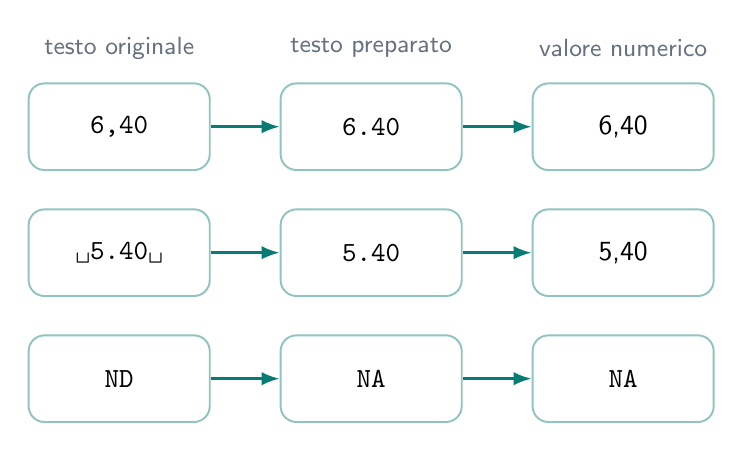
\begin{tikzpicture}[x=1cm,y=1cm]
\foreach \yy/\t/\s/\v in {3.3/{\texttt{6,40}}/{\texttt{6.40}}/{6,40},1.7/{\texttt{\char32 5.40\char32}}/{\texttt{5.40}}/{5,40},.1/{\texttt{ND}}/{\texttt{NA}}/{\texttt{NA}}}{
 \node[pFlow,minimum width=2.3cm] (a) at(1.4,\yy){\t};
 \node[pFlow,minimum width=2.3cm] (b) at(4.6,\yy){\s};
 \node[pFlow,minimum width=2.3cm] (c) at(7.8,\yy){\v};
 \draw[pEdge](a)--(b);\draw[pEdge](b)--(c);}
\node[pNote] at(1.4,4.3){testo originale};\node[pNote] at(4.6,4.3){testo preparato};\node[pNote] at(7.8,4.3){valore numerico};
\end{tikzpicture}
\PSmall{\texttt{trimws()} elimina spazi alle estremità. \texttt{sub()} sostituisce la prima virgola con un punto. Il codice tratta scritture decimali semplici, senza separatori delle migliaia.}

\end{minipage}% 
\end{lrbox}
\typeout{FULLBOX:019:L:\the\ht\PilotLeftBox:\the\dp\PilotLeftBox}
\begin{lrbox}{\PilotRightBox}%
\begin{minipage}[t]{7.55cm}\raggedright\color{Ink}\fontsize{11.3}{14.8}\selectfont

\PCode{R · una conversione controllabile}{19_numeri.R}
\PSmall{\texttt{NA\_character\_} è un mancante testuale. \texttt{as.numeric()} tenta la conversione numerica. \texttt{originale} rimane invariato.}
\PInfo{Questo esempio riconosce \texttt{ND} come codice di indisponibilità. La convenzione deve essere documentata per il dataset utilizzato.}

\end{minipage}% 
\end{lrbox}
\typeout{FULLBOX:019:R:\the\ht\PilotRightBox:\the\dp\PilotRightBox}
\begin{frame}[plain]\hypertarget{slide19}{}
\bookmark[level=1,page=19]{Conversione dei numeri e codici dichiarati}
\begin{tikzpicture}[remember picture,overlay]
\PilotChrome{Conversione dei numeri e codici dichiarati}{IMPORTAZIONE E CONVERSIONI}{19}{Una conversione deve conservare il significato dei codici speciali e permettere il confronto con il testo iniziale.}
\node[anchor=north west,inner sep=0] at ([xshift=0.96cm,yshift=-2.13cm]current page.north west) {\usebox{\PilotLeftBox}};
\node[anchor=north west,inner sep=0] at ([xshift=11.52cm,yshift=-2.13cm]current page.north west) {\usebox{\PilotRightBox}};

\end{tikzpicture}\end{frame}

% SLIDE 020 | Zero, dato assente e limite di misura
\begin{lrbox}{\PilotLeftBox}%
\begin{minipage}[t]{10.05cm}\raggedright\color{Ink}\fontsize{11.3}{14.8}\selectfont

\PLabel{Registrazioni con informazioni differenti}
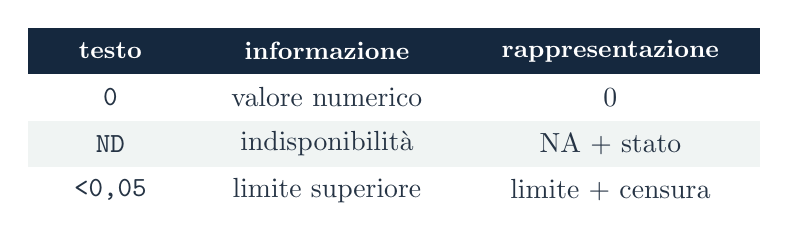
\begin{tikzpicture}[x=1cm,y=1cm]
\fill[Navy] (0,0) rectangle (9.3,0.59);
\node[font=\bfseries\fontsize{9.2}{11}\selectfont,text=white] at (1.05,0.295) {testo};
\node[font=\bfseries\fontsize{9.2}{11}\selectfont,text=white] at (3.8,0.295) {informazione};
\node[font=\bfseries\fontsize{9.2}{11}\selectfont,text=white] at (7.4,0.295) {rappresentazione};
\fill[white] (0,-0.59) rectangle (9.3,0.0);
\node[font=\fontsize{9.6}{12}\selectfont,text=Ink] at (1.05,-0.295) {\texttt{0}};
\node[font=\fontsize{9.6}{12}\selectfont,text=Ink] at (3.8,-0.295) {valore numerico};
\node[font=\fontsize{9.6}{12}\selectfont,text=Ink] at (7.4,-0.295) {0};
\fill[GeoTint] (0,-1.18) rectangle (9.3,-0.59);
\node[font=\fontsize{9.6}{12}\selectfont,text=Ink] at (1.05,-0.885) {\texttt{ND}};
\node[font=\fontsize{9.6}{12}\selectfont,text=Ink] at (3.8,-0.885) {indisponibilità};
\node[font=\fontsize{9.6}{12}\selectfont,text=Ink] at (7.4,-0.885) {NA + stato};
\fill[white] (0,-1.77) rectangle (9.3,-1.1800000000000002);
\node[font=\fontsize{9.6}{12}\selectfont,text=Ink] at (1.05,-1.475) {\texttt{<0,05}};
\node[font=\fontsize{9.6}{12}\selectfont,text=Ink] at (3.8,-1.475) {limite superiore};
\node[font=\fontsize{9.6}{12}\selectfont,text=Ink] at (7.4,-1.475) {limite + censura};
\end{tikzpicture}
\vspace{4mm}\PBody{Sostituire una misura assente con zero aggiunge un'informazione non osservata. Eliminare il simbolo \texttt{<} trasforma invece un limite in una misura puntuale.}
\PSmall{I tre casi sono illustrativi. Nel CSV dei fossili, \texttt{ND} compare nel diametro esterno di F002; la cella vuota di F006 riguarda il diaframma.}
\PSmall{\texttt{ND} indica qui indisponibilità. Il significato del codice può cambiare fra laboratori; la censura è documentata in un file separato.}

\end{minipage}% 
\end{lrbox}
\typeout{FULLBOX:020:L:\the\ht\PilotLeftBox:\the\dp\PilotLeftBox}
\begin{lrbox}{\PilotRightBox}%
\begin{minipage}[t]{7.55cm}\raggedright\color{Ink}\fontsize{11.3}{14.8}\selectfont

\PCode{R · verificare un codice dichiarato}{20_mancanti_dichiarati.R}
\PBody{\texttt{is.na(0)} è falso. La disponibilità di una misura e il suo valore sono proprietà distinte.}

\end{minipage}% 
\end{lrbox}
\typeout{FULLBOX:020:R:\the\ht\PilotRightBox:\the\dp\PilotRightBox}
\begin{frame}[plain]\hypertarget{slide20}{}
\bookmark[level=1,page=20]{Zero, dato assente e limite di misura}
\begin{tikzpicture}[remember picture,overlay]
\PilotChrome{Zero, dato assente e limite di misura}{IMPORTAZIONE E CONVERSIONI}{20}{Distinguere un valore nullo, una misura indisponibile e un’informazione espressa come limite.}
\node[anchor=north west,inner sep=0] at ([xshift=0.96cm,yshift=-2.13cm]current page.north west) {\usebox{\PilotLeftBox}};
\node[anchor=north west,inner sep=0] at ([xshift=11.52cm,yshift=-2.13cm]current page.north west) {\usebox{\PilotRightBox}};

\end{tikzpicture}\end{frame}

% SLIDE 021 | Esiti della conversione e anomalie di formato
\begin{lrbox}{\PilotLeftBox}%
\begin{minipage}[t]{10.05cm}\raggedright\color{Ink}\fontsize{11.3}{14.8}\selectfont

\PLabel{NA non descrive da solo la causa}
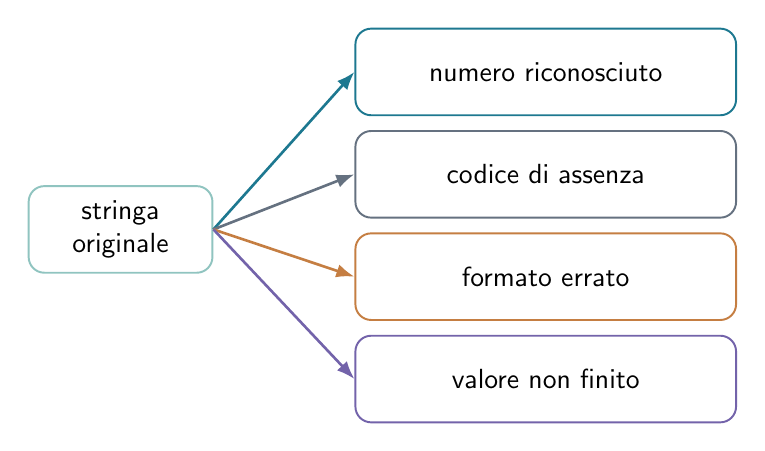
\begin{tikzpicture}[x=1cm,y=1cm]
\node[pFlow,text width=2.1cm] (s) at(1.3,2){stringa\\originale};
\foreach \yy/\txt/\col in {4/{numero riconosciuto}/GeoA,2.7/{codice di assenza}/Muted,1.4/{formato errato}/GeoB,.1/{valore non finito}/GeoC}{
 \node[pFlow,text width=4.6cm,draw=\col] (z) at(6.7,\yy){\txt};\draw[pEdge,\col](s.east)--(z.west);}
\end{tikzpicture}
\PBody{La funzione \texttt{converti\_misura()} restituisce valore e stato. Il suo codice, in \texttt{setup.R}, controlla la scrittura numerica e conserva separatamente anche i limiti censurati.}

\end{minipage}% 
\end{lrbox}
\typeout{FULLBOX:021:L:\the\ht\PilotLeftBox:\the\dp\PilotLeftBox}
\begin{lrbox}{\PilotRightBox}%
\begin{minipage}[t]{7.55cm}\raggedright\color{Ink}\fontsize{11.3}{14.8}\selectfont

\PCode{R · interrogare gli esiti}{21_esiti_conversione.R}
\PSmall{\texttt{z\$valore} e \texttt{z\$stato} estraggono dalla lista i due risultati per ogni stringa.}
\PInfo{\texttt{Inf} non è una misura finita. Al controllo della scrittura deve seguire quello del dominio fisico.}
\PSmall{\texttt{errore} è aggiunto appositamente. Il CSV originale non contiene conversioni fallite.}

\end{minipage}% 
\end{lrbox}
\typeout{FULLBOX:021:R:\the\ht\PilotRightBox:\the\dp\PilotRightBox}
\begin{frame}[plain]\hypertarget{slide21}{}
\bookmark[level=1,page=21]{Esiti della conversione e anomalie di formato}
\begin{tikzpicture}[remember picture,overlay]
\PilotChrome{Esiti della conversione e anomalie di formato}{IMPORTAZIONE E CONVERSIONI}{21}{Registrare l’esito della conversione consente di distinguere assenza dichiarata, formato errato e valori non finiti.}
\node[anchor=north west,inner sep=0] at ([xshift=0.96cm,yshift=-2.13cm]current page.north west) {\usebox{\PilotLeftBox}};
\node[anchor=north west,inner sep=0] at ([xshift=11.52cm,yshift=-2.13cm]current page.north west) {\usebox{\PilotRightBox}};

\end{tikzpicture}\end{frame}

% SLIDE 022 | Conservare il limite e il segno della censura
\begin{lrbox}{\PilotLeftBox}%
\begin{minipage}[t]{10.05cm}\raggedright\color{Ink}\fontsize{11.3}{14.8}\selectfont

\PLabel{Una misura inferiore al limite}
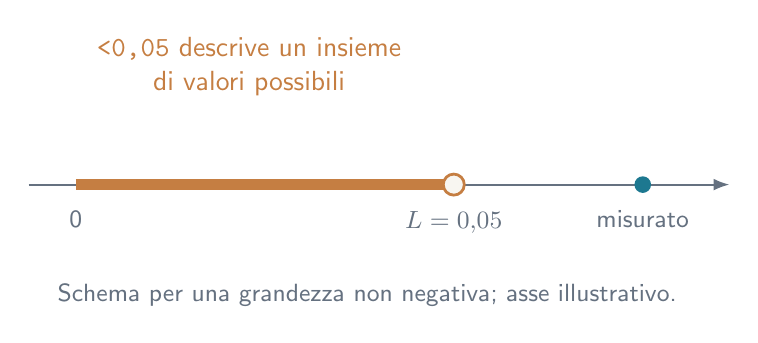
\begin{tikzpicture}[x=1cm,y=1cm]
\draw[pAxis](.4,1.5)--(9.3,1.5);
\draw[GeoB,line width=4pt](1,1.5)--(5.8,1.5);
\draw[GeoB,fill=Paper,line width=1pt](5.8,1.5)circle(3.8pt);
\fill[GeoA](8.2,1.5)circle(3pt);
\node[pNote,below=6pt] at(1,1.5){0};
\node[pNote,below=6pt] at(5.8,1.5){$L=0{,}05$};
\node[pNote,below=6pt] at(8.2,1.5){misurato};
\node[pLabel,text width=5cm,text=GeoB] at(3.2,3){\texttt{<0,05} descrive un insieme\\di valori possibili};
\node[pNote] at(4.7,.1){Schema per una grandezza non negativa; asse illustrativo.};
\end{tikzpicture}
\PBody{La registrazione conserva $x<L$, con $L$ noto. La sostituzione con $L$, $L/2$ o zero introduce un'ipotesi aggiuntiva.}
\PSmall{Il file didattico sulla censura non specifica un'unità fisica: qui si discutono solo i valori numerici e il loro stato.}

\end{minipage}% 
\end{lrbox}
\typeout{FULLBOX:022:L:\the\ht\PilotLeftBox:\the\dp\PilotLeftBox}
\begin{lrbox}{\PilotRightBox}%
\begin{minipage}[t]{7.55cm}\raggedright\color{Ink}\fontsize{11.3}{14.8}\selectfont

\PCode{R · valore, limite e stato}{22_limiti.R}
\PBody{Per il dato censurato, \texttt{valore} è \texttt{NA}; \texttt{limite} conserva 0,05 e \texttt{z\$operatore} il segno.}
\PInfo{Un limite quantitativo contiene più informazione di un semplice dato assente. Il trattamento successivo dipende dall'analisi e dalle ipotesi.}

\end{minipage}% 
\end{lrbox}
\typeout{FULLBOX:022:R:\the\ht\PilotRightBox:\the\dp\PilotRightBox}
\begin{frame}[plain]\hypertarget{slide22}{}
\bookmark[level=1,page=22]{Conservare il limite e il segno della censura}
\begin{tikzpicture}[remember picture,overlay]
\PilotChrome{Conservare il limite e il segno della censura}{IMPORTAZIONE E CONVERSIONI}{22}{Conservare insieme testo, limite e stato della misura censurata, senza trasformare implicitamente il limite in un’osservazione.}
\node[anchor=north west,inner sep=0] at ([xshift=0.96cm,yshift=-2.13cm]current page.north west) {\usebox{\PilotLeftBox}};
\node[anchor=north west,inner sep=0] at ([xshift=11.52cm,yshift=-2.13cm]current page.north west) {\usebox{\PilotRightBox}};

\end{tikzpicture}\end{frame}

% SLIDE 023 | Nomi, unità e dizionario delle variabili
\begin{lrbox}{\PilotLeftBox}%
\begin{minipage}[t]{10.05cm}\raggedright\color{Ink}\fontsize{11.3}{14.8}\selectfont

\PLabel{Il nome della colonna accompagna una definizione}
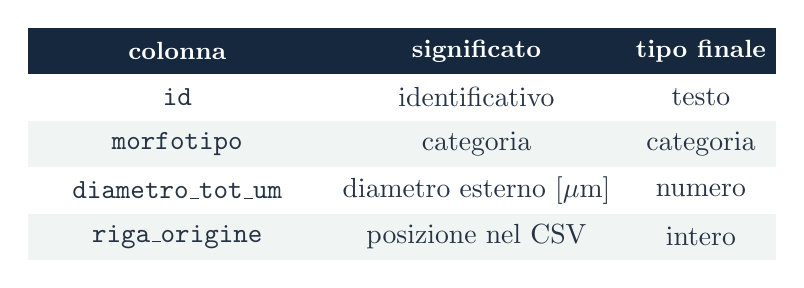
\begin{tikzpicture}[x=1cm,y=1cm]
\fill[Navy] (0,0) rectangle (9.5,0.59);
\node[font=\bfseries\fontsize{9.2}{11}\selectfont,text=white] at (1.9,0.295) {colonna};
\node[font=\bfseries\fontsize{9.2}{11}\selectfont,text=white] at (5.699999999999999,0.295) {significato};
\node[font=\bfseries\fontsize{9.2}{11}\selectfont,text=white] at (8.549999999999999,0.295) {tipo finale};
\fill[white] (0,-0.59) rectangle (9.5,0.0);
\node[font=\fontsize{9.6}{12}\selectfont,text=Ink] at (1.9,-0.295) {\texttt{id}};
\node[font=\fontsize{9.6}{12}\selectfont,text=Ink] at (5.699999999999999,-0.295) {identificativo};
\node[font=\fontsize{9.6}{12}\selectfont,text=Ink] at (8.549999999999999,-0.295) {testo};
\fill[GeoTint] (0,-1.18) rectangle (9.5,-0.59);
\node[font=\fontsize{9.6}{12}\selectfont,text=Ink] at (1.9,-0.885) {\texttt{morfotipo}};
\node[font=\fontsize{9.6}{12}\selectfont,text=Ink] at (5.699999999999999,-0.885) {categoria};
\node[font=\fontsize{9.6}{12}\selectfont,text=Ink] at (8.549999999999999,-0.885) {categoria};
\fill[white] (0,-1.77) rectangle (9.5,-1.1800000000000002);
\node[font=\fontsize{9.6}{12}\selectfont,text=Ink] at (1.9,-1.475) {\texttt{diametro\_tot\_um}};
\node[font=\fontsize{9.6}{12}\selectfont,text=Ink] at (5.699999999999999,-1.475) {diametro esterno [$\mu$m]};
\node[font=\fontsize{9.6}{12}\selectfont,text=Ink] at (8.549999999999999,-1.475) {numero};
\fill[GeoTint] (0,-2.36) rectangle (9.5,-1.77);
\node[font=\fontsize{9.6}{12}\selectfont,text=Ink] at (1.9,-2.065) {\texttt{riga\_origine}};
\node[font=\fontsize{9.6}{12}\selectfont,text=Ink] at (5.699999999999999,-2.065) {posizione nel CSV};
\node[font=\fontsize{9.6}{12}\selectfont,text=Ink] at (8.549999999999999,-2.065) {intero};
\end{tikzpicture}
\vspace{3mm}\PBody{Una definizione comprende unità, codici ammessi e significato dei mancanti. Un nome corretto non garantisce che i valori abbiano il tipo o l'unità prevista.}
\PSmall{I diametri e il diaframma sono in micrometri. Nel progetto, la prima lettura è testuale; il dizionario descrive anche il significato dopo la conversione.}

\end{minipage}% 
\end{lrbox}
\typeout{FULLBOX:023:L:\the\ht\PilotLeftBox:\the\dp\PilotLeftBox}
\begin{lrbox}{\PilotRightBox}%
\begin{minipage}[t]{7.55cm}\raggedright\color{Ink}\fontsize{11.3}{14.8}\selectfont

\PCode{R · una specifica minima della struttura}{23_dizionario.R}
\PSmall{\texttt{all()} richiede che ogni nome sia presente. \texttt{vapply()} applica un controllo a ciascuna colonna, richiedendo un singolo risultato logico.}
\PInfo{Il numero di riga è intero; le cinque colonne di origine rimangono testuali.}

\end{minipage}% 
\end{lrbox}
\typeout{FULLBOX:023:R:\the\ht\PilotRightBox:\the\dp\PilotRightBox}
\begin{frame}[plain]\hypertarget{slide23}{}
\bookmark[level=1,page=23]{Nomi, unità e dizionario delle variabili}
\begin{tikzpicture}[remember picture,overlay]
\PilotChrome{Nomi, unità e dizionario delle variabili}{IMPORTAZIONE E CONVERSIONI}{23}{Il dizionario descrive le variabili; i controlli di struttura verificano che la tabella corrisponda a quella descrizione.}
\node[anchor=north west,inner sep=0] at ([xshift=0.96cm,yshift=-2.13cm]current page.north west) {\usebox{\PilotLeftBox}};
\node[anchor=north west,inner sep=0] at ([xshift=11.52cm,yshift=-2.13cm]current page.north west) {\usebox{\PilotRightBox}};

\end{tikzpicture}\end{frame}

% SLIDE 024 | Riepilogo delle conversioni
\begin{lrbox}{\PilotLeftBox}%
\begin{minipage}[t]{10.05cm}\raggedright\color{Ink}\fontsize{11.3}{14.8}\selectfont

\PLabel{Confrontare forma iniziale e tabella derivata}
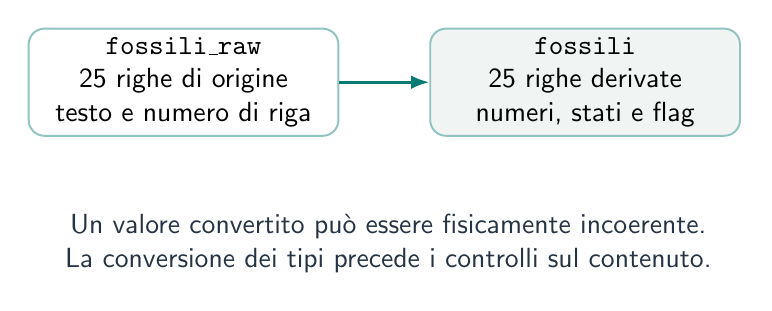
\begin{tikzpicture}[x=1cm,y=1cm]
\node[pFlow,text width=3.7cm] (r) at(2.1,2.7){\texttt{fossili\_raw}\\25 righe di origine\\testo e numero di riga};
\node[pFlow,text width=3.7cm,fill=GeoTint] (d) at(7.2,2.7){\texttt{fossili}\\25 righe derivate\\numeri, stati e flag};
\draw[pEdge](r)--(d);
\node[pLabel,text width=8.8cm] at(4.7,.65){Un valore convertito può essere fisicamente incoerente. La conversione dei tipi precede i controlli sul contenuto.};
\end{tikzpicture}
\PBody{Per esempio, il diametro esterno di F004 viene letto come $-5{,}1\ \mu$m. La scrittura è numerica; il segno viola il dominio di una lunghezza.}
\PInfo{Nel CSV non si osservano errori di formato. Le anomalie presenti riguardano disponibilità, geometria e duplicazione.}

\end{minipage}% 
\end{lrbox}
\typeout{FULLBOX:024:L:\the\ht\PilotLeftBox:\the\dp\PilotLeftBox}
\begin{lrbox}{\PilotRightBox}%
\begin{minipage}[t]{7.55cm}\raggedright\color{Ink}\fontsize{11.3}{14.8}\selectfont

\PCode{R · contare senza perdere le righe}{24_riepilogo_conversioni.R}
\PSmall{\texttt{[[v]]} estrae la colonna il cui nome è conservato in \texttt{v}. \texttt{useNA="ifany"} rende visibili eventuali mancanti nel conteggio.}
\PSmall{\texttt{prepara\_fossili()} conserva tutte le righe e aggiunge colonne di stato. La sezione sui controlli ne esamina le regole.}

\end{minipage}% 
\end{lrbox}
\typeout{FULLBOX:024:R:\the\ht\PilotRightBox:\the\dp\PilotRightBox}
\begin{frame}[plain]\hypertarget{slide24}{}
\bookmark[level=1,page=24]{Riepilogo delle conversioni}
\begin{tikzpicture}[remember picture,overlay]
\PilotChrome{Riepilogo delle conversioni}{IMPORTAZIONE E CONVERSIONI}{24}{Una tabella numerica può ancora contenere dati incoerenti: separare la verifica del formato dalla verifica scientifica.}
\node[anchor=north west,inner sep=0] at ([xshift=0.96cm,yshift=-2.13cm]current page.north west) {\usebox{\PilotLeftBox}};
\node[anchor=north west,inner sep=0] at ([xshift=11.52cm,yshift=-2.13cm]current page.north west) {\usebox{\PilotRightBox}};

\end{tikzpicture}\end{frame}

% SLIDE 025 | Tellus: diagnosticare una convenzione errata
\begin{lrbox}{\PilotLeftBox}%
\begin{minipage}[t]{10.05cm}\raggedright\color{Ink}\fontsize{11.3}{14.8}\selectfont

\PLabel{Stesso testo, due esiti di lettura}
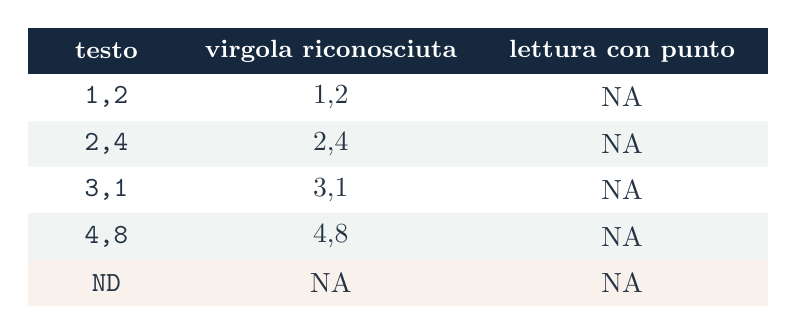
\begin{tikzpicture}[x=1cm,y=1cm]
\fill[Navy] (0,0) rectangle (9.4,0.59);
\node[font=\bfseries\fontsize{9.2}{11}\selectfont,text=white] at (1.0,0.295) {testo};
\node[font=\bfseries\fontsize{9.2}{11}\selectfont,text=white] at (3.85,0.295) {virgola riconosciuta};
\node[font=\bfseries\fontsize{9.2}{11}\selectfont,text=white] at (7.550000000000001,0.295) {lettura con punto};
\fill[white] (0,-0.59) rectangle (9.4,0.0);
\node[font=\fontsize{9.6}{12}\selectfont,text=Ink] at (1.0,-0.295) {\texttt{1,2}};
\node[font=\fontsize{9.6}{12}\selectfont,text=Ink] at (3.85,-0.295) {1,2};
\node[font=\fontsize{9.6}{12}\selectfont,text=Ink] at (7.550000000000001,-0.295) {NA};
\fill[GeoTint] (0,-1.18) rectangle (9.4,-0.59);
\node[font=\fontsize{9.6}{12}\selectfont,text=Ink] at (1.0,-0.885) {\texttt{2,4}};
\node[font=\fontsize{9.6}{12}\selectfont,text=Ink] at (3.85,-0.885) {2,4};
\node[font=\fontsize{9.6}{12}\selectfont,text=Ink] at (7.550000000000001,-0.885) {NA};
\fill[white] (0,-1.77) rectangle (9.4,-1.1800000000000002);
\node[font=\fontsize{9.6}{12}\selectfont,text=Ink] at (1.0,-1.475) {\texttt{3,1}};
\node[font=\fontsize{9.6}{12}\selectfont,text=Ink] at (3.85,-1.475) {3,1};
\node[font=\fontsize{9.6}{12}\selectfont,text=Ink] at (7.550000000000001,-1.475) {NA};
\fill[GeoTint] (0,-2.36) rectangle (9.4,-1.77);
\node[font=\fontsize{9.6}{12}\selectfont,text=Ink] at (1.0,-2.065) {\texttt{4,8}};
\node[font=\fontsize{9.6}{12}\selectfont,text=Ink] at (3.85,-2.065) {4,8};
\node[font=\fontsize{9.6}{12}\selectfont,text=Ink] at (7.550000000000001,-2.065) {NA};
\fill[GeoB!10] (0,-2.9499999999999997) rectangle (9.4,-2.36);
\node[font=\fontsize{9.6}{12}\selectfont,text=Ink] at (1.0,-2.655) {\texttt{ND}};
\node[font=\fontsize{9.6}{12}\selectfont,text=Ink] at (3.85,-2.655) {NA};
\node[font=\fontsize{9.6}{12}\selectfont,text=Ink] at (7.550000000000001,-2.655) {NA};
\end{tikzpicture}
\vspace{3mm}\PBody{Nel sito, alternare \emph{Virgola} e \emph{Punto}. Annotare quante conversioni riescono e se la media può essere calcolata.}
\PSmall{Il caso è deterministico. Il cambio del seme non modifica le cinque stringhe predisposte.}

\end{minipage}% 
\end{lrbox}
\typeout{FULLBOX:025:L:\the\ht\PilotLeftBox:\the\dp\PilotLeftBox}
\begin{lrbox}{\PilotRightBox}%
\begin{minipage}[t]{7.55cm}\raggedright\color{Ink}\fontsize{11.3}{14.8}\selectfont

\PCode{R · controllare la lettura corretta}{25_lab_importazione.R}
\PBody{Con la virgola si ottengono quattro valori e media 2,875. Con il punto nessuna stringa è convertita: la media è indefinita.}
\vspace{3mm}\PBody{\href{https://marzione00.github.io/Lab_Geo/\#laboratorio/m02-importazione}{Apri l'esperimento M02 · Importazione}}
\PSmall{Consegna: distinguere il dato indisponibile dai quattro numeri resi mancanti da una convenzione incompatibile.}

\end{minipage}% 
\end{lrbox}
\typeout{FULLBOX:025:R:\the\ht\PilotRightBox:\the\dp\PilotRightBox}
\begin{frame}[plain]\hypertarget{slide25}{}
\bookmark[level=1,page=25]{Tellus: diagnosticare una convenzione errata}
\begin{tikzpicture}[remember picture,overlay]
\PilotChrome{Tellus: diagnosticare una convenzione errata}{LABORATORIO · IMPORTAZIONE}{25}{Contare i valori convertiti prima di calcolare una sintesi; una media assente può dipendere dalla lettura del file.}
\node[anchor=north west,inner sep=0] at ([xshift=0.96cm,yshift=-2.13cm]current page.north west) {\usebox{\PilotLeftBox}};
\node[anchor=north west,inner sep=0] at ([xshift=11.52cm,yshift=-2.13cm]current page.north west) {\usebox{\PilotRightBox}};

\end{tikzpicture}\end{frame}

% SLIDE 026 | Variabili derivate: massa, volume e densità
\begin{lrbox}{\PilotLeftBox}%
\begin{minipage}[t]{10.05cm}\raggedright\color{Ink}\fontsize{11.3}{14.8}\selectfont

\PLabel{Le due misure devono appartenere allo stesso provino}
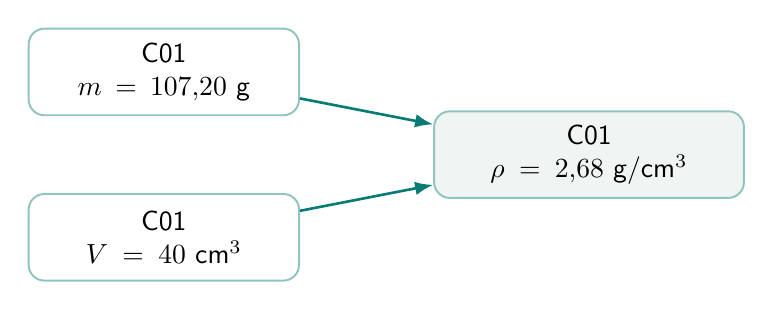
\begin{tikzpicture}[x=1cm,y=1cm]
\node[pFlow,text width=3.2cm] (m) at(1.8,3.2){C01\\$m=107{,}20$ g};
\node[pFlow,text width=3.2cm] (v) at(1.8,1.1){C01\\$V=40$ cm$^3$};
\node[pFlow,text width=3.7cm,fill=GeoTint] (d) at(7.2,2.15){C01\\$\rho=2{,}68$ g/cm$^3$};
\draw[pEdge](m)--(d);\draw[pEdge](v)--(d);
\end{tikzpicture}
\[\rho_i=\frac{m_i}{V_i},\qquad V_i>0.\]
\PSmall{$i$ identifica il provino. Con massa in g e volume in cm$^3$, il rapporto è in g/cm$^3$. Il significato fisico dipende da quale volume è stato misurato.}

\end{minipage}% 
\end{lrbox}
\typeout{FULLBOX:026:L:\the\ht\PilotLeftBox:\the\dp\PilotLeftBox}
\begin{lrbox}{\PilotRightBox}%
\begin{minipage}[t]{7.55cm}\raggedright\color{Ink}\fontsize{11.3}{14.8}\selectfont

\PCode{R · aggiungere una colonna derivata}{26_densita.R}
\PBody{\texttt{/} divide elemento per elemento. Il risultato resta associato all'identificativo del provino.}
\PInfo{Metodo di misura e volume usato stabiliscono se il rapporto descrive una densità apparente o dei granuli.}

\end{minipage}% 
\end{lrbox}
\typeout{FULLBOX:026:R:\the\ht\PilotRightBox:\the\dp\PilotRightBox}
\begin{frame}[plain]\hypertarget{slide26}{}
\bookmark[level=1,page=26]{Variabili derivate: massa, volume e densità}
\begin{tikzpicture}[remember picture,overlay]
\PilotChrome{Variabili derivate: massa, volume e densità}{TRASFORMAZIONI E AGGREGAZIONI}{26}{Una variabile derivata richiede misure compatibili, unità dichiarate e corrispondenza fra numeratore e denominatore.}
\node[anchor=north west,inner sep=0] at ([xshift=0.96cm,yshift=-2.13cm]current page.north west) {\usebox{\PilotLeftBox}};
\node[anchor=north west,inner sep=0] at ([xshift=11.52cm,yshift=-2.13cm]current page.north west) {\usebox{\PilotRightBox}};

\end{tikzpicture}\end{frame}

% SLIDE 027 | Riciclo dei vettori e abbinamento delle misure
\begin{lrbox}{\PilotLeftBox}%
\begin{minipage}[t]{10.05cm}\raggedright\color{Ink}\fontsize{11.3}{14.8}\selectfont

\PLabel{La regola del linguaggio può produrre un rapporto non voluto}
\begin{tikzpicture}[x=1cm,y=1cm]
\foreach \xx/\m/\v in {1.2/10/2,3.4/20/5,5.6/30/2,7.8/40/5}{
 \node[pFlow,minimum width=1.6cm] (a) at(\xx,3){$\m$};
 \node[pFlow,minimum width=1.6cm] (b) at(\xx,1.3){$\v$};
 \draw[pEdge](a)--(b);}
\draw[GeoB,dashed,thick,rounded corners=2mm](4.6,.6)rectangle(8.8,2);
\node[pNote,text=GeoB] at(6.7,-.05){valori ripetuti da R};
\node[pNote] at(4.5,4){quattro masse e soltanto due volumi};
\end{tikzpicture}
\PBody{R ripete il vettore più corto, senza avvertimenti quando le due lunghezze sono multiple.}
\PSmall{Lo schema mostra il comportamento numerico; non costituisce un insieme valido di coppie massa-volume di quattro provini.}

\end{minipage}% 
\end{lrbox}
\typeout{FULLBOX:027:L:\the\ht\PilotLeftBox:\the\dp\PilotLeftBox}
\begin{lrbox}{\PilotRightBox}%
\begin{minipage}[t]{7.55cm}\raggedright\color{Ink}\fontsize{11.3}{14.8}\selectfont

\PCode{R · riconoscere una lunghezza errata}{27_riciclo.R}
\PSmall{Avere uguale lunghezza è necessario per questo calcolo, ma non basta: ordine e identificativi devono garantire che ogni coppia si riferisca allo stesso provino.}

\end{minipage}% 
\end{lrbox}
\typeout{FULLBOX:027:R:\the\ht\PilotRightBox:\the\dp\PilotRightBox}
\begin{frame}[plain]\hypertarget{slide27}{}
\bookmark[level=1,page=27]{Riciclo dei vettori e abbinamento delle misure}
\begin{tikzpicture}[remember picture,overlay]
\PilotChrome{Riciclo dei vettori e abbinamento delle misure}{TRASFORMAZIONI E AGGREGAZIONI}{27}{L’assenza di un avvertimento non dimostra che due vettori rappresentino misure correttamente abbinate.}
\node[anchor=north west,inner sep=0] at ([xshift=0.96cm,yshift=-2.13cm]current page.north west) {\usebox{\PilotLeftBox}};
\node[anchor=north west,inner sep=0] at ([xshift=11.52cm,yshift=-2.13cm]current page.north west) {\usebox{\PilotRightBox}};

\end{tikzpicture}\end{frame}

% SLIDE 028 | Aggregazione e unità della tabella
\begin{lrbox}{\PilotLeftBox}%
\begin{minipage}[t]{10.05cm}\raggedright\color{Ink}\fontsize{11.3}{14.8}\selectfont

\PLabel{Quattro provini diventano una sintesi di stazione}
\begin{tikzpicture}[x=1cm,y=1cm]
\foreach \yy/\id/\v in {3.8/C01/{2,68},2.6/C02/{2,71},1.4/C03/{2,65},.2/C04/{2,70}}{
 \node[pFlow,minimum width=3.3cm,minimum height=.85cm] (a) at(1.9,\yy){\id\quad $\rho=\v$};
 \draw[pEdge](a.east)--(5.1,2);}
\node[pFlow,text width=3.7cm,fill=GeoTint] at(7.3,2){stazione A1\\$n=4$\\$\bar\rho=2{,}685$ g/cm$^3$};
\end{tikzpicture}
\PBody{Dopo l'aggregazione una riga rappresenta una stazione. La sua numerosità e la sua media riassumono i provini disponibili in quel gruppo.}
\PSmall{Valori delle prime quattro righe del CSV; densità in g/cm$^3$.}

\end{minipage}% 
\end{lrbox}
\typeout{FULLBOX:028:L:\the\ht\PilotLeftBox:\the\dp\PilotLeftBox}
\begin{lrbox}{\PilotRightBox}%
\begin{minipage}[t]{7.55cm}\raggedright\color{Ink}\fontsize{11.3}{14.8}\selectfont

\PCode{R · calcolare una media per gruppo}{28_aggregare.R}
\[\bar\rho_g=\frac{1}{n_g}\sum_{i\in g}\rho_i.\]
\PSmall{$g$ identifica una stazione; $n_g$ conta le misure usate. Qui i 24 valori sono tutti disponibili, in sei gruppi da quattro provini.}
\PBody{\texttt{densita \textasciitilde{} stazione} indica variabile e gruppo; \texttt{FUN=mean} sceglie la sintesi.}

\end{minipage}% 
\end{lrbox}
\typeout{FULLBOX:028:R:\the\ht\PilotRightBox:\the\dp\PilotRightBox}
\begin{frame}[plain]\hypertarget{slide28}{}
\bookmark[level=1,page=28]{Aggregazione e unità della tabella}
\begin{tikzpicture}[remember picture,overlay]
\PilotChrome{Aggregazione e unità della tabella}{TRASFORMAZIONI E AGGREGAZIONI}{28}{L’aggregazione modifica il significato della riga: conservare chiave, numerosità e definizione della sintesi.}
\node[anchor=north west,inner sep=0] at ([xshift=0.96cm,yshift=-2.13cm]current page.north west) {\usebox{\PilotLeftBox}};
\node[anchor=north west,inner sep=0] at ([xshift=11.52cm,yshift=-2.13cm]current page.north west) {\usebox{\PilotRightBox}};

\end{tikzpicture}\end{frame}

% SLIDE 029 | Il denominatore della sintesi
\begin{lrbox}{\PilotLeftBox}%
\begin{minipage}[t]{10.05cm}\raggedright\color{Ink}\fontsize{11.3}{14.8}\selectfont

\PLabel{Registrazioni raccolte e valori usati}
\begin{tikzpicture}[x=1cm,y=1cm]
\fill[Navy] (0,0) rectangle (9.0,0.59);
\node[font=\bfseries\fontsize{9.2}{11}\selectfont,text=white] at (1.0,0.295) {riga};
\node[font=\bfseries\fontsize{9.2}{11}\selectfont,text=white] at (3.75,0.295) {valore};
\node[font=\bfseries\fontsize{9.2}{11}\selectfont,text=white] at (7.25,0.295) {usato};
\fill[white] (0,-0.59) rectangle (9.0,0.0);
\node[font=\fontsize{9.6}{12}\selectfont,text=Ink] at (1.0,-0.295) {1};
\node[font=\fontsize{9.6}{12}\selectfont,text=Ink] at (3.75,-0.295) {2};
\node[font=\fontsize{9.6}{12}\selectfont,text=Ink] at (7.25,-0.295) {sì};
\fill[GeoB!10] (0,-1.18) rectangle (9.0,-0.59);
\node[font=\fontsize{9.6}{12}\selectfont,text=Ink] at (1.0,-0.885) {2};
\node[font=\fontsize{9.6}{12}\selectfont,text=Ink] at (3.75,-0.885) {NA};
\node[font=\fontsize{9.6}{12}\selectfont,text=Ink] at (7.25,-0.885) {no};
\fill[white] (0,-1.77) rectangle (9.0,-1.1800000000000002);
\node[font=\fontsize{9.6}{12}\selectfont,text=Ink] at (1.0,-1.475) {3};
\node[font=\fontsize{9.6}{12}\selectfont,text=Ink] at (3.75,-1.475) {4};
\node[font=\fontsize{9.6}{12}\selectfont,text=Ink] at (7.25,-1.475) {sì};
\end{tikzpicture}
\vspace{2.5mm}
\[\mathcal O_g=\{i\in g:x_i\ \text{disponibile}\},\qquad
 \bar x_{g,\rm obs}=\frac{\sum_{i\in\mathcal O_g}x_i}{|\mathcal O_g|}.\]
\PSmall{$\mathcal O_g$ è l'insieme dei valori utilizzati nel gruppo; $|\mathcal O_g|$ la sua numerosità. La media richiede $|\mathcal O_g|>0$.}
\PBody{Nell'esempio, dividere per tre tratterebbe implicitamente il mancante come uno zero.}
\PSmall{Senza valori disponibili, la media è indefinita. Il conteggio totale documenta comunque la copertura.}

\end{minipage}% 
\end{lrbox}
\typeout{FULLBOX:029:L:\the\ht\PilotLeftBox:\the\dp\PilotLeftBox}
\begin{lrbox}{\PilotRightBox}%
\begin{minipage}[t]{7.55cm}\raggedright\color{Ink}\fontsize{11.3}{14.8}\selectfont

\PCode{R · riportare entrambi i conteggi}{29_denominatore.R}
\PBody{\texttt{is.finite()} riconosce numeri finiti e restituisce falso per \texttt{NA}, \texttt{NaN} e infinito. La regola deve essere adeguata alla variabile.}

\end{minipage}% 
\end{lrbox}
\typeout{FULLBOX:029:R:\the\ht\PilotRightBox:\the\dp\PilotRightBox}
\begin{frame}[plain]\hypertarget{slide29}{}
\bookmark[level=1,page=29]{Il denominatore della sintesi}
\begin{tikzpicture}[remember picture,overlay]
\PilotChrome{Il denominatore della sintesi}{TRASFORMAZIONI E AGGREGAZIONI}{29}{Ogni sintesi deve riportare il numero delle registrazioni e quello dei valori effettivamente usati nel calcolo.}
\node[anchor=north west,inner sep=0] at ([xshift=0.96cm,yshift=-2.13cm]current page.north west) {\usebox{\PilotLeftBox}};
\node[anchor=north west,inner sep=0] at ([xshift=11.52cm,yshift=-2.13cm]current page.north west) {\usebox{\PilotRightBox}};

\end{tikzpicture}\end{frame}

% SLIDE 030 | Medie di gruppo e pesi
\begin{lrbox}{\PilotLeftBox}%
\begin{minipage}[t]{10.05cm}\raggedright\color{Ink}\fontsize{11.3}{14.8}\selectfont

\PLabel{Il raccordo con Terra 01}
\begin{tikzpicture}[x=1cm,y=1cm]
\node[pLabel,anchor=west] at(0,3.2){Media delle osservazioni};
\fill[GeoA](0,2.2)rectangle(7.5,2.85);\fill[GeoB](7.5,2.2)rectangle(9,2.85);
\node[font=\bfseries,text=white] at(3.75,2.52){A: $5/6$};\node[font=\bfseries,text=white] at(8.25,2.52){B: $1/6$};
\node[pLabel,anchor=west] at(0,1.35){Media delle medie di gruppo};
\fill[GeoA](0,.35)rectangle(4.5,1);\fill[GeoB](4.5,.35)rectangle(9,1);
\node[font=\bfseries,text=white] at(2.25,.68){A: $1/2$};\node[font=\bfseries,text=white] at(6.75,.68){B: $1/2$};
\end{tikzpicture}
\PSmall{Pesi illustrati per i gruppi del laboratorio Tellus: 50 misure in A e 10 in B. Nei provini del CSV le sei stazioni sono invece bilanciate.}
\[\bar x=\sum_g\frac{n_g}{N}\bar x_g,\qquad
\bar x_{\rm gruppi}=\frac{1}{G}\sum_g\bar x_g.\]
\PSmall{$N=\sum_g n_g$ è il totale usato; $G$ il numero di gruppi. I pesi della prima media dipendono dalle numerosità.}

\end{minipage}% 
\end{lrbox}
\typeout{FULLBOX:030:L:\the\ht\PilotLeftBox:\the\dp\PilotLeftBox}
\begin{lrbox}{\PilotRightBox}%
\begin{minipage}[t]{7.55cm}\raggedright\color{Ink}\fontsize{11.3}{14.8}\selectfont

\PCode{R · ricostruire la media complessiva}{30_pesi.R}
\PInfo{\texttt{n[names(m)]} allinea i conteggi ai nomi delle medie. Con mancanti, i conteggi devono riguardare gli stessi valori usati per calcolare ciascuna media.}

\end{minipage}% 
\end{lrbox}
\typeout{FULLBOX:030:R:\the\ht\PilotRightBox:\the\dp\PilotRightBox}
\begin{frame}[plain]\hypertarget{slide30}{}
\bookmark[level=1,page=30]{Medie di gruppo e pesi}
\begin{tikzpicture}[remember picture,overlay]
\PilotChrome{Medie di gruppo e pesi}{TRASFORMAZIONI E AGGREGAZIONI}{30}{La media delle medie coincide con quella delle osservazioni quando i gruppi usati hanno uguale numerosità.}
\node[anchor=north west,inner sep=0] at ([xshift=0.96cm,yshift=-2.13cm]current page.north west) {\usebox{\PilotLeftBox}};
\node[anchor=north west,inner sep=0] at ([xshift=11.52cm,yshift=-2.13cm]current page.north west) {\usebox{\PilotRightBox}};

\end{tikzpicture}\end{frame}

% SLIDE 031 | Formato largo e formato lungo
\begin{lrbox}{\PilotLeftBox}%
\begin{minipage}[t]{10.05cm}\raggedright\color{Ink}\fontsize{11.3}{14.8}\selectfont

\PLabel{Il numero di righe dipende da che cosa rappresentano}
\begin{tikzpicture}[x=1cm,y=1cm]
\fill[Navy] (0,0) rectangle (9.0,0.59);
\node[font=\bfseries\fontsize{9.2}{11}\selectfont,text=white] at (1.0,0.295) {id};
\node[font=\bfseries\fontsize{9.2}{11}\selectfont,text=white] at (3.75,0.295) {massa [g]};
\node[font=\bfseries\fontsize{9.2}{11}\selectfont,text=white] at (7.25,0.295) {volume [cm$^3$]};
\fill[white] (0,-0.59) rectangle (9.0,0.0);
\node[font=\fontsize{9.6}{12}\selectfont,text=Ink] at (1.0,-0.295) {C01};
\node[font=\fontsize{9.6}{12}\selectfont,text=Ink] at (3.75,-0.295) {107,20};
\node[font=\fontsize{9.6}{12}\selectfont,text=Ink] at (7.25,-0.295) {40};
\fill[GeoTint] (0,-1.18) rectangle (9.0,-0.59);
\node[font=\fontsize{9.6}{12}\selectfont,text=Ink] at (1.0,-0.885) {C02};
\node[font=\fontsize{9.6}{12}\selectfont,text=Ink] at (3.75,-0.885) {121,95};
\node[font=\fontsize{9.6}{12}\selectfont,text=Ink] at (7.25,-0.885) {45};
\end{tikzpicture}
\vspace{3mm}\PSmall{Una riga per provino; una colonna per variabile.}
\vspace{3mm}
\begin{tikzpicture}[x=1cm,y=1cm]
\fill[Navy] (0,0) rectangle (9,0.59);
\node[font=\bfseries\fontsize{9.2}{11}\selectfont,text=white] at (1.0,0.295) {id};
\node[font=\bfseries\fontsize{9.2}{11}\selectfont,text=white] at (4.0,0.295) {variabile};
\node[font=\bfseries\fontsize{9.2}{11}\selectfont,text=white] at (7.5,0.295) {valore};
\fill[white] (0,-0.59) rectangle (9,0.0);
\node[font=\fontsize{9.6}{12}\selectfont,text=Ink] at (1.0,-0.295) {C01};
\node[font=\fontsize{9.6}{12}\selectfont,text=Ink] at (4.0,-0.295) {\texttt{massa\_g}};
\node[font=\fontsize{9.6}{12}\selectfont,text=Ink] at (7.5,-0.295) {107,20};
\fill[GeoTint] (0,-1.18) rectangle (9,-0.59);
\node[font=\fontsize{9.6}{12}\selectfont,text=Ink] at (1.0,-0.885) {C01};
\node[font=\fontsize{9.6}{12}\selectfont,text=Ink] at (4.0,-0.885) {\texttt{volume\_cm3}};
\node[font=\fontsize{9.6}{12}\selectfont,text=Ink] at (7.5,-0.885) {40};
\fill[white] (0,-1.77) rectangle (9,-1.1800000000000002);
\node[font=\fontsize{9.6}{12}\selectfont,text=Ink] at (1.0,-1.475) {C02};
\node[font=\fontsize{9.6}{12}\selectfont,text=Ink] at (4.0,-1.475) {\texttt{massa\_g}};
\node[font=\fontsize{9.6}{12}\selectfont,text=Ink] at (7.5,-1.475) {121,95};
\fill[GeoTint] (0,-2.36) rectangle (9,-1.77);
\node[font=\fontsize{9.6}{12}\selectfont,text=Ink] at (1.0,-2.065) {C02};
\node[font=\fontsize{9.6}{12}\selectfont,text=Ink] at (4.0,-2.065) {\texttt{volume\_cm3}};
\node[font=\fontsize{9.6}{12}\selectfont,text=Ink] at (7.5,-2.065) {45};
\end{tikzpicture}
\PSmall{Una riga per coppia provino-variabile. Il significato e l'unità accompagnano ogni valore.}

\end{minipage}% 
\end{lrbox}
\typeout{FULLBOX:031:L:\the\ht\PilotLeftBox:\the\dp\PilotLeftBox}
\begin{lrbox}{\PilotRightBox}%
\begin{minipage}[t]{7.55cm}\raggedright\color{Ink}\fontsize{11.3}{14.8}\selectfont

\PCode{R · riorganizzare due colonne}{31_formato_lungo.R}
\PSmall{\texttt{varying} indica le colonne da riunire; \texttt{v.names} nomina il valore; \texttt{timevar} nomina la colonna che le distingue. Qui non rappresenta un tempo.}
\PBody{La chiave diventa la coppia \texttt{id, variabile}. Il numero di provini rimane 24, mentre le righe diventano 48.}

\end{minipage}% 
\end{lrbox}
\typeout{FULLBOX:031:R:\the\ht\PilotRightBox:\the\dp\PilotRightBox}
\begin{frame}[plain]\hypertarget{slide31}{}
\bookmark[level=1,page=31]{Formato largo e formato lungo}
\begin{tikzpicture}[remember picture,overlay]
\PilotChrome{Formato largo e formato lungo}{TRASFORMAZIONI E AGGREGAZIONI}{31}{Cambiare formato modifica la struttura della tabella; il numero di unità osservate deve rimanere riconoscibile.}
\node[anchor=north west,inner sep=0] at ([xshift=0.96cm,yshift=-2.13cm]current page.north west) {\usebox{\PilotLeftBox}};
\node[anchor=north west,inner sep=0] at ([xshift=11.52cm,yshift=-2.13cm]current page.north west) {\usebox{\PilotRightBox}};

\end{tikzpicture}\end{frame}

% SLIDE 032 | Controllare una trasformazione di formato
\begin{lrbox}{\PilotLeftBox}%
\begin{minipage}[t]{10.05cm}\raggedright\color{Ink}\fontsize{11.3}{14.8}\selectfont

\PLabel{Tre proprietà da confrontare}
\begin{tikzpicture}[x=1cm,y=1cm]
\node[pFlow,text width=3.4cm] (a) at(2,3.2){\textbf{Unità osservate}\\24 identificativi di provino};
\node[pFlow,text width=3.4cm] (b) at(7.2,3.2){\textbf{Righe}\\$24\times2=48$ coppie};
\node[pFlow,text width=7.7cm,fill=GeoTint] (c) at(4.6,1.1){\textbf{Chiave}\quad (identificativo, variabile)\\Una sola registrazione per ogni coppia attesa};
\draw[pEdge](a.south)--(c.north west);\draw[pEdge](b.south)--(c.north east);
\end{tikzpicture}
\PBody{Una colonna che riunisce masse e volumi richiede una colonna per la variabile e una per l'unità. Una media indiscriminata di quei valori non avrebbe un'unità coerente.}
\PSmall{Qui ogni provino ha due variabili: il formato lungo conserva una riga per ciascuna coppia, anche quando il valore è \texttt{NA}.}

\end{minipage}% 
\end{lrbox}
\typeout{FULLBOX:032:L:\the\ht\PilotLeftBox:\the\dp\PilotLeftBox}
\begin{lrbox}{\PilotRightBox}%
\begin{minipage}[t]{7.55cm}\raggedright\color{Ink}\fontsize{11.3}{14.8}\selectfont

\PCode{R · verificare chiave e unità}{32_verificare_formato.R}
\PSmall{\texttt{ifelse()} sceglie un valore per ciascuna riga. \texttt{anyDuplicated()} segnala se la chiave composta compare più volte.}

\end{minipage}% 
\end{lrbox}
\typeout{FULLBOX:032:R:\the\ht\PilotRightBox:\the\dp\PilotRightBox}
\begin{frame}[plain]\hypertarget{slide32}{}
\bookmark[level=1,page=32]{Controllare una trasformazione di formato}
\begin{tikzpicture}[remember picture,overlay]
\PilotChrome{Controllare una trasformazione di formato}{TRASFORMAZIONI E AGGREGAZIONI}{32}{Dopo una trasformazione, verificare unità osservate, chiavi, numerosità e unità di misura.}
\node[anchor=north west,inner sep=0] at ([xshift=0.96cm,yshift=-2.13cm]current page.north west) {\usebox{\PilotLeftBox}};
\node[anchor=north west,inner sep=0] at ([xshift=11.52cm,yshift=-2.13cm]current page.north west) {\usebox{\PilotRightBox}};

\end{tikzpicture}\end{frame}

% SLIDE 033 | Tellus: gruppi sbilanciati e due medie
\begin{lrbox}{\PilotLeftBox}%
\begin{minipage}[t]{10.05cm}\raggedright\color{Ink}\fontsize{11.3}{14.8}\selectfont

\PLabel{Il modello del secondo modulo}
\PBody{Il sito genera due gruppi indipendenti: A ha media 3, B media 8; la deviazione standard è 1 in entrambi. Varia $n_A$, mentre B conserva 10 misure.}
\[E(\bar X)=\frac{3n_A+80}{n_A+10},\qquad
 E(\bar X_{\rm gruppi})=\frac{3+8}{2}=5{,}5.\]
\begin{tikzpicture}[x=1cm,y=1cm]
\fill[Navy] (0,0) rectangle (9.4,0.59);
\node[font=\bfseries\fontsize{9.2}{11}\selectfont,text=white] at (1.0,0.295) {$n_A$};
\node[font=\bfseries\fontsize{9.2}{11}\selectfont,text=white] at (3.5,0.295) {peso di A};
\node[font=\bfseries\fontsize{9.2}{11}\selectfont,text=white] at (7.2,0.295) {attesa media misure};
\fill[white] (0,-0.59) rectangle (9.4,0.0);
\node[font=\fontsize{9.6}{12}\selectfont,text=Ink] at (1.0,-0.295) {10};
\node[font=\fontsize{9.6}{12}\selectfont,text=Ink] at (3.5,-0.295) {1/2};
\node[font=\fontsize{9.6}{12}\selectfont,text=Ink] at (7.2,-0.295) {5,50};
\fill[GeoTint] (0,-1.18) rectangle (9.4,-0.59);
\node[font=\fontsize{9.6}{12}\selectfont,text=Ink] at (1.0,-0.885) {50};
\node[font=\fontsize{9.6}{12}\selectfont,text=Ink] at (3.5,-0.885) {5/6};
\node[font=\fontsize{9.6}{12}\selectfont,text=Ink] at (7.2,-0.885) {3,83};
\fill[white] (0,-1.77) rectangle (9.4,-1.1800000000000002);
\node[font=\fontsize{9.6}{12}\selectfont,text=Ink] at (1.0,-1.475) {100};
\node[font=\fontsize{9.6}{12}\selectfont,text=Ink] at (3.5,-1.475) {10/11};
\node[font=\fontsize{9.6}{12}\selectfont,text=Ink] at (7.2,-1.475) {3,45};
\end{tikzpicture}
\vspace{3mm}\PSmall{Attese del modello, arrotondate; il singolo campione produce valori differenti. Con uguali numerosità le due statistiche coincidono sullo stesso campione.}

\end{minipage}% 
\end{lrbox}
\typeout{FULLBOX:033:L:\the\ht\PilotLeftBox:\the\dp\PilotLeftBox}
\begin{lrbox}{\PilotRightBox}%
\begin{minipage}[t]{7.55cm}\raggedright\color{Ink}\fontsize{11.3}{14.8}\selectfont

\PCode{R · confrontare campione e attesa}{33_lab_aggregazioni.R}
\PSmall{Il file contiene il generatore completo. Il seme fissa la sequenza; cambiare $n_A$ cambia anche le estrazioni per B.}
\vspace{2mm}\PSmall{\href{https://marzione00.github.io/Lab_Geo/\#laboratorio/m02-aggregazioni}{Apri il laboratorio di aggregazione}}
\PSmall{Consegna: confrontare $n_A=10,50,100$ con le attese e motivare la scelta dei pesi.}

\end{minipage}% 
\end{lrbox}
\typeout{FULLBOX:033:R:\the\ht\PilotRightBox:\the\dp\PilotRightBox}
\begin{frame}[plain]\hypertarget{slide33}{}
\bookmark[level=1,page=33]{Tellus: gruppi sbilanciati e due medie}
\begin{tikzpicture}[remember picture,overlay]
\PilotChrome{Tellus: gruppi sbilanciati e due medie}{LABORATORIO · AGGREGAZIONI}{33}{Il parametro del gruppo A cambia i pesi della media complessiva; la media dei gruppi assegna metà del peso a ciascuno.}
\node[anchor=north west,inner sep=0] at ([xshift=0.96cm,yshift=-2.13cm]current page.north west) {\usebox{\PilotLeftBox}};
\node[anchor=north west,inner sep=0] at ([xshift=11.52cm,yshift=-2.13cm]current page.north west) {\usebox{\PilotRightBox}};

\end{tikzpicture}\end{frame}

% SLIDE 034 | Identificativi e unità della tabella
\begin{lrbox}{\PilotLeftBox}%
\begin{minipage}[t]{10.05cm}\raggedright\color{Ink}\fontsize{11.3}{14.8}\selectfont

\PLabel{Una riga per provino; una riga per sito}
\begin{tikzpicture}[x=1cm,y=1cm]
 \fill[Navy] (0,3.15) rectangle (4.45,3.8);
 \fill[Navy] (5.65,3.15) rectangle (9.5,3.8);
 \node[pLabel,text=white] at (2.2,3.48) {Provini};
 \node[pLabel,text=white] at (7.58,3.48) {Siti};
 \node[pLabel] at (.95,2.77) {\textbf{id}};
 \node[pLabel] at (3.25,2.77) {sito};
 \node[pLabel] at (6.6,2.77) {\textbf{sito}};
 \node[pLabel] at (8.55,2.77) {quota [m]};
 \foreach \id/\s/\yy in {p1/A/2.05,p2/A/1.35,p3/B/.65}{
  \draw[Rule] (0,\yy-.33)--(4.45,\yy-.33);
  \node[pLabel,text=GeoA] at (.95,\yy) {\id};
  \node[pLabel] at (3.25,\yy) {\s};
 }
 \foreach \s/\q/\yy in {A/10/2.05,B/20/1.35}{
  \draw[Rule] (5.65,\yy-.33)--(9.5,\yy-.33);
  \node[pLabel,text=GeoB] at (6.6,\yy) {\s};
  \node[pLabel] at (8.55,\yy) {\q};
 }
 \draw[GeoA,rounded corners=1mm] (.35,.27) rectangle (1.55,2.42);
 \draw[GeoB,rounded corners=1mm] (6.05,.98) rectangle (7.15,2.42);
\end{tikzpicture}
\PBody{\texttt{id} distingue i provini. Il codice del sito si ripete perché due provini provengono da A. Nella tabella dei siti, A compare una sola volta.}
\PSmall{Esempio minimo costruito per il collegamento; le quote sono illustrative.}

\end{minipage}% 
\end{lrbox}
\typeout{FULLBOX:034:L:\the\ht\PilotLeftBox:\the\dp\PilotLeftBox}
\begin{lrbox}{\PilotRightBox}%
\begin{minipage}[t]{7.55cm}\raggedright\color{Ink}\fontsize{11.3}{14.8}\selectfont

\PCode{R · due tabelle di esempio}{34_tabelle.R}
\PSmall{I nomi \texttt{provini} e \texttt{siti} restano disponibili nelle slide successive. Le due tabelle rappresentano unità diverse.}
\PInfo{Prima di scegliere la chiave, scrivere che cosa rappresenta ogni riga. Una chiave può comprendere più colonne.}

\end{minipage}% 
\end{lrbox}
\typeout{FULLBOX:034:R:\the\ht\PilotRightBox:\the\dp\PilotRightBox}
\begin{frame}[plain]\hypertarget{slide34}{}
\bookmark[level=1,page=34]{Identificativi e unità della tabella}
\begin{tikzpicture}[remember picture,overlay]
\PilotChrome{Identificativi e unità della tabella}{CHIAVI E RELAZIONI}{34}{L'unicità di una chiave si valuta rispetto all'unità rappresentata dalla tabella.}
\node[anchor=north west,inner sep=0] at ([xshift=0.96cm,yshift=-2.13cm]current page.north west) {\usebox{\PilotLeftBox}};
\node[anchor=north west,inner sep=0] at ([xshift=11.52cm,yshift=-2.13cm]current page.north west) {\usebox{\PilotRightBox}};

\end{tikzpicture}\end{frame}

% SLIDE 035 | Una chiave completa e univoca
\begin{lrbox}{\PilotLeftBox}%
\begin{minipage}[t]{10.05cm}\raggedright\color{Ink}\fontsize{11.3}{14.8}\selectfont

\PLabel{Due controlli distinti}
\begin{tikzpicture}[x=1cm,y=1cm]
 \node[pFlow,text width=2.5cm] (k) at (1.55,2.5) {Colonna\\\texttt{sito}};
 \node[pFlow,text width=4.8cm] (a) at (6.7,3.5) {Completezza\\nessun \texttt{NA} o codice vuoto};
 \node[pFlow,text width=4.8cm] (b) at (6.7,1.35) {Unicità\\nessun codice ripetuto};
 \draw[pEdge] (k.east)--(3.4,2.5)|-(a.west);
 \draw[pEdge] (k.east)--(3.4,2.5)|-(b.west);
 \node[pNote] at (4.85,.2) {Entrambe le condizioni riguardano la tabella dei siti.};
\end{tikzpicture}
\[k(u)=k(v)\ \Longrightarrow\ u=v.\]
\PSmall{$k$ associa un codice a ogni sito; $u$ e $v$ sono siti. Due siti distinti devono avere codici distinti.}

\end{minipage}% 
\end{lrbox}
\typeout{FULLBOX:035:L:\the\ht\PilotLeftBox:\the\dp\PilotLeftBox}
\begin{lrbox}{\PilotRightBox}%
\begin{minipage}[t]{7.55cm}\raggedright\color{Ink}\fontsize{11.3}{14.8}\selectfont

\PCode{R · verificare l'anagrafica}{35_chiave.R}
\PSmall{\texttt{anyNA()} trova valori mancanti. \texttt{nzchar()} riconosce stringhe non vuote; \texttt{trimws()} rimuove spazi ai bordi. \texttt{anyDuplicated()} restituisce zero se non ci sono duplicati.}
\PInfo{\texttt{merge()} può abbinare fra loro anche chiavi \texttt{NA}. Per questa anagrafica i codici mancanti non sono ammessi.}

\end{minipage}% 
\end{lrbox}
\typeout{FULLBOX:035:R:\the\ht\PilotRightBox:\the\dp\PilotRightBox}
\begin{frame}[plain]\hypertarget{slide35}{}
\bookmark[level=1,page=35]{Una chiave completa e univoca}
\begin{tikzpicture}[remember picture,overlay]
\PilotChrome{Una chiave completa e univoca}{CHIAVI E RELAZIONI}{35}{Verificare sia i codici assenti sia quelli ripetuti prima di collegare una tabella di riferimento.}
\node[anchor=north west,inner sep=0] at ([xshift=0.96cm,yshift=-2.13cm]current page.north west) {\usebox{\PilotLeftBox}};
\node[anchor=north west,inner sep=0] at ([xshift=11.52cm,yshift=-2.13cm]current page.north west) {\usebox{\PilotRightBox}};

\end{tikzpicture}\end{frame}

% SLIDE 036 | Cardinalità di una relazione
\begin{lrbox}{\PilotLeftBox}%
\begin{minipage}[t]{10.05cm}\raggedright\color{Ink}\fontsize{11.3}{14.8}\selectfont

\PLabel{Quante righe corrispondono alla stessa chiave?}
\begin{tikzpicture}[x=1cm,y=1cm]
 \foreach \yy/\lab in {4.0/Uno a uno,2.15/Molti a uno,.3/Molti a molti}{
  \node[pLabel,anchor=west] at (0,\yy) {\lab};
 }
 \node[pFlow,minimum width=1.3cm,minimum height=.6cm] (a1) at (4.3,4) {A};
 \node[pFlow,minimum width=1.3cm,minimum height=.6cm] (b1) at (8,4) {A};
 \draw[pEdge] (a1)--(b1);
 \foreach \yy/\nm in {2.55/a2,1.75/a3}
  \node[pFlow,minimum width=1.3cm,minimum height=.6cm] (\nm) at (4.3,\yy) {A};
 \node[pFlow,minimum width=1.3cm,minimum height=.6cm] (b2) at (8,2.15) {A};
 \draw[pEdge] (a2.east)--(b2.west);\draw[pEdge] (a3.east)--(b2.west);
 \foreach \yy/\nm in {.7/a4,-.1/a5}
  \node[pFlow,minimum width=1.3cm,minimum height=.6cm] (\nm) at (4.3,\yy) {A};
 \foreach \yy/\nm in {.7/b4,-.1/b5}
  \node[pFlow,minimum width=1.3cm,minimum height=.6cm] (\nm) at (8,\yy) {A};
 \foreach \a in {a4,a5}\foreach \b in {b4,b5}\draw[pEdge,draw=GeoB] (\a.east)--(\b.west);
\end{tikzpicture}
\PSmall{Ogni rettangolo è una riga. Le frecce rappresentano le coppie che il collegamento produce per la chiave A.}

\end{minipage}% 
\end{lrbox}
\typeout{FULLBOX:036:L:\the\ht\PilotLeftBox:\the\dp\PilotLeftBox}
\begin{lrbox}{\PilotRightBox}%
\begin{minipage}[t]{7.55cm}\raggedright\color{Ink}\fontsize{11.3}{14.8}\selectfont

\PLabel{La relazione attesa}
\PBody{Provini e anagrafica dei siti formano una relazione molti-a-uno: ciascun provino appartiene a un sito, ciascun sito può avere più provini.}
\vspace{3mm}
\PBody{Se una tabella contiene campagne successive, la chiave può richiedere sito e data. Collegare soltanto per sito produce tutte le combinazioni compatibili.}
\PInfo{La relazione molti-a-molti è appropriata quando quelle combinazioni hanno un significato previsto. Negli altri casi segnala una chiave incompleta o una duplicazione.}

\end{minipage}% 
\end{lrbox}
\typeout{FULLBOX:036:R:\the\ht\PilotRightBox:\the\dp\PilotRightBox}
\begin{frame}[plain]\hypertarget{slide36}{}
\bookmark[level=1,page=36]{Cardinalità di una relazione}
\begin{tikzpicture}[remember picture,overlay]
\PilotChrome{Cardinalità di una relazione}{CHIAVI E RELAZIONI}{36}{Dichiarare la cardinalità attesa consente di riconoscere un collegamento che cambia il significato delle righe.}
\node[anchor=north west,inner sep=0] at ([xshift=0.96cm,yshift=-2.13cm]current page.north west) {\usebox{\PilotLeftBox}};
\node[anchor=north west,inner sep=0] at ([xshift=11.52cm,yshift=-2.13cm]current page.north west) {\usebox{\PilotRightBox}};

\end{tikzpicture}\end{frame}

% SLIDE 037 | Collegare i provini ai metadati del sito
\begin{lrbox}{\PilotLeftBox}%
\begin{minipage}[t]{10.05cm}\raggedright\color{Ink}\fontsize{11.3}{14.8}\selectfont

\PLabel{Collegamento molti-a-uno}
\begin{tikzpicture}[x=1cm,y=1cm]
 \foreach \id/\ss/\yy in {p1/A/3.5,p2/A/2.35,p3/B/1.2}{
  \node[pFlow,minimum width=2.7cm,minimum height=.7cm] (\id) at (1.7,\yy) {\id\quad\textbf{\ss}};
 }
 \node[pFlow,text width=2.7cm,minimum height=.8cm] (a) at (7.6,3.0) {\textbf{A}\quad10 m};
 \node[pFlow,text width=2.7cm,minimum height=.8cm] (b) at (7.6,1.2) {\textbf{B}\quad20 m};
 \draw[pEdge] (p1.east)--(a.west);\draw[pEdge] (p2.east)--(a.west);
 \draw[pEdge] (p3.east)--(b.west);
 \node[pNote] at (4.65,.25) {La quota di A viene associata a entrambi i suoi provini.};
\end{tikzpicture}
\PBody{Il risultato conserva tre provini e aggiunge una colonna. La quota è una proprietà del sito: ripeterla nelle due righe non crea una nuova misura di quota.}

\end{minipage}% 
\end{lrbox}
\typeout{FULLBOX:037:L:\the\ht\PilotLeftBox:\the\dp\PilotLeftBox}
\begin{lrbox}{\PilotRightBox}%
\begin{minipage}[t]{7.55cm}\raggedright\color{Ink}\fontsize{11.3}{14.8}\selectfont

\PCode{R · aggiungere una colonna}{37_join.R}
\PSmall{\texttt{by} indica la chiave. \texttt{all.x=TRUE} conserva ogni riga della tabella a sinistra. L'unicità dei siti è stata controllata nella slide 35.}
\PInfo{Controllare le chiavi prive di corrispondenza. Un \texttt{NA} nella quota può anche essere già presente nei metadati: le due situazioni richiedono verifiche diverse.}

\end{minipage}% 
\end{lrbox}
\typeout{FULLBOX:037:R:\the\ht\PilotRightBox:\the\dp\PilotRightBox}
\begin{frame}[plain]\hypertarget{slide37}{}
\bookmark[level=1,page=37]{Collegare i provini ai metadati del sito}
\begin{tikzpicture}[remember picture,overlay]
\PilotChrome{Collegare i provini ai metadati del sito}{CHIAVI E RELAZIONI}{37}{Un collegamento molti-a-uno con chiavi complete deve conservare il numero delle righe della tabella dei provini.}
\node[anchor=north west,inner sep=0] at ([xshift=0.96cm,yshift=-2.13cm]current page.north west) {\usebox{\PilotLeftBox}};
\node[anchor=north west,inner sep=0] at ([xshift=11.52cm,yshift=-2.13cm]current page.north west) {\usebox{\PilotRightBox}};

\end{tikzpicture}\end{frame}

% SLIDE 038 | Una chiave duplicata moltiplica le righe
\begin{lrbox}{\PilotLeftBox}%
\begin{minipage}[t]{10.05cm}\raggedright\color{Ink}\fontsize{11.3}{14.8}\selectfont

\PLabel{Due provini A e due registrazioni per A}
\begin{tikzpicture}[x=1cm,y=1cm]
 \node[pFlow,minimum width=2.3cm,minimum height=.8cm] (p1) at (1.4,3.5) {p1 · A};
 \node[pFlow,minimum width=2.3cm,minimum height=.8cm] (p2) at (1.4,1.8) {p2 · A};
 \node[pFlow,minimum width=2.3cm,minimum height=.8cm] (a1) at (5.05,3.5) {A · 10 m};
 \node[pFlow,minimum width=2.3cm,minimum height=.8cm] (a2) at (5.05,1.8) {A · 12 m};
 \foreach \p in {p1,p2}\foreach \a in {a1,a2}\draw[pEdge,draw=GeoB] (\p.east)--(\a.west);
 \node[pLabel,text width=2.2cm] at (8,2.65) {\textbf{4 righe}\\per A};
 \node[pNote] at (4.55,.6) {B compare una volta su ogni lato: aggiunge una riga.};
\end{tikzpicture}
\[n_{\mathrm{inner}}=\sum_k n_L(k)n_R(k)=2\cdot2+1\cdot1=5.\]
\PSmall{$k$: chiave condivisa; $n_L(k)$ e $n_R(k)$: sue occorrenze nelle due tabelle. La formula riguarda un \emph{inner join}.}

\end{minipage}% 
\end{lrbox}
\typeout{FULLBOX:038:L:\the\ht\PilotLeftBox:\the\dp\PilotLeftBox}
\begin{lrbox}{\PilotRightBox}%
\begin{minipage}[t]{7.55cm}\raggedright\color{Ink}\fontsize{11.3}{14.8}\selectfont

\PCode{R · osservare la moltiplicazione}{38_molteplicita.R}
\PSmall{\texttt{rbind()} aggiunge una riga. Le due quote di A producono due abbinamenti per ogni provino A.}
\PInfo{Con un collegamento sinistro, una chiave senza corrispondenza conserva comunque le proprie righe, con metadati mancanti.}

\end{minipage}% 
\end{lrbox}
\typeout{FULLBOX:038:R:\the\ht\PilotRightBox:\the\dp\PilotRightBox}
\begin{frame}[plain]\hypertarget{slide38}{}
\bookmark[level=1,page=38]{Una chiave duplicata moltiplica le righe}
\begin{tikzpicture}[remember picture,overlay]
\PilotChrome{Una chiave duplicata moltiplica le righe}{CHIAVI E RELAZIONI}{38}{Il numero di righe dopo un join dipende dalle molteplicità delle chiavi sui due lati.}
\node[anchor=north west,inner sep=0] at ([xshift=0.96cm,yshift=-2.13cm]current page.north west) {\usebox{\PilotLeftBox}};
\node[anchor=north west,inner sep=0] at ([xshift=11.52cm,yshift=-2.13cm]current page.north west) {\usebox{\PilotRightBox}};

\end{tikzpicture}\end{frame}

% SLIDE 039 | Chiavi senza corrispondenza
\begin{lrbox}{\PilotLeftBox}%
\begin{minipage}[t]{10.05cm}\raggedright\color{Ink}\fontsize{11.3}{14.8}\selectfont

\PLabel{Conservare e riconoscere le righe non abbinate}
\begin{tikzpicture}[x=1cm,y=1cm]
 \node[pFlow,text width=3cm] (p) at (1.9,3.4) {Provini\\p1: A · p2: A · p3: B};
 \node[pFlow,text width=3cm] (s) at (7.5,3.4) {Siti disponibili\\A: 10 m};
 \node[pFlow,text width=7.7cm,minimum height=1.2cm] (j) at (4.7,1.15) {p1: A, 10 m\qquad p2: A, 10 m\\\textcolor{GeoB}{p3: B, NA}};
 \draw[pEdge] (p.south)--(p.south |- j.north);
 \draw[pEdge] (s.south)--(s.south |- j.north);
 \node[pNote,text=GeoB] at (4.7,.1) {B è presente nei provini e assente nell'anagrafica.};
\end{tikzpicture}
\PBody{Una corrispondenza assente può dipendere da un codice diverso, da una registrazione mancante o da una copertura incompleta della seconda tabella.}

\end{minipage}% 
\end{lrbox}
\typeout{FULLBOX:039:L:\the\ht\PilotLeftBox:\the\dp\PilotLeftBox}
\begin{lrbox}{\PilotRightBox}%
\begin{minipage}[t]{7.55cm}\raggedright\color{Ink}\fontsize{11.3}{14.8}\selectfont

\PCode{R · cercare i codici assenti}{39_non_abbinati.R}
\PSmall{\texttt{setdiff(x,y)} restituisce i valori presenti in \texttt{x} e assenti in \texttt{y}. Il controllo riguarda le chiavi, prima di leggere gli attributi aggiunti.}
\PInfo{La somiglianza tra due nomi non basta a identificarli. Uniformare i codici solo quando la corrispondenza è documentata.}

\end{minipage}% 
\end{lrbox}
\typeout{FULLBOX:039:R:\the\ht\PilotRightBox:\the\dp\PilotRightBox}
\begin{frame}[plain]\hypertarget{slide39}{}
\bookmark[level=1,page=39]{Chiavi senza corrispondenza}
\begin{tikzpicture}[remember picture,overlay]
\PilotChrome{Chiavi senza corrispondenza}{CHIAVI E RELAZIONI}{39}{Registrare le chiavi non abbinate permette di distinguere un problema di collegamento da un valore mancante nei metadati.}
\node[anchor=north west,inner sep=0] at ([xshift=0.96cm,yshift=-2.13cm]current page.north west) {\usebox{\PilotLeftBox}};
\node[anchor=north west,inner sep=0] at ([xshift=11.52cm,yshift=-2.13cm]current page.north west) {\usebox{\PilotRightBox}};

\end{tikzpicture}\end{frame}

% SLIDE 040 | Duplicati e misure ripetute
\begin{lrbox}{\PilotLeftBox}%
\begin{minipage}[t]{10.05cm}\raggedright\color{Ink}\fontsize{11.3}{14.8}\selectfont

\PLabel{Il confronto deve rispettare la definizione della riga}
\begin{tikzpicture}[x=1cm,y=1cm]
 \node[pLabel,anchor=west] at (0,3.9) {Duplicato esatto};
 \node[pFlow,text width=3.7cm,minimum height=.8cm] (a) at (2,3.0) {p1 · 12/05 · 8,0};
 \node[pFlow,text width=3.7cm,minimum height=.8cm] (b) at (7.2,3.0) {p1 · 12/05 · 8,0};
 \draw[GeoB,line width=1.0pt] (a.east)--node[pNote,above]{uguali}(b.west);
 \node[pLabel,anchor=west] at (0,1.85) {Misura in un'altra occasione};
 \node[pFlow,text width=3.7cm,minimum height=.8cm] (c) at (2,.95) {p1 · 12/05 · 8,0};
 \node[pFlow,text width=3.7cm,minimum height=.8cm] (d) at (7.2,.95) {p1 · 19/05 · 8,2};
 \node[pNote] at (4.6,.0) {Nel secondo caso, la chiave comprende id e data.};
\end{tikzpicture}
\PBody{L'identificativo ripetuto segnala una condizione da esaminare. La ripetizione può rappresentare una replica prevista dal protocollo.}

\end{minipage}% 
\end{lrbox}
\typeout{FULLBOX:040:L:\the\ht\PilotLeftBox:\the\dp\PilotLeftBox}
\begin{lrbox}{\PilotRightBox}%
\begin{minipage}[t]{7.55cm}\raggedright\color{Ink}\fontsize{11.3}{14.8}\selectfont

\PCode{R · due definizioni di duplicato}{40_duplicati.R}
\PSmall{Escludere \texttt{riga\_origine} dal confronto esatto. \texttt{fromLast=TRUE} segnala anche la prima occorrenza degli identificativi ripetuti.}
\PInfo{F007 è un duplicato esatto. Nell'esercizio si conserva la prima occorrenza e si segnala la successiva.}

\end{minipage}% 
\end{lrbox}
\typeout{FULLBOX:040:R:\the\ht\PilotRightBox:\the\dp\PilotRightBox}
\begin{frame}[plain]\hypertarget{slide40}{}
\bookmark[level=1,page=40]{Duplicati e misure ripetute}
\begin{tikzpicture}[remember picture,overlay]
\PilotChrome{Duplicati e misure ripetute}{CHIAVI E RELAZIONI}{40}{Definire la chiave e le colonne confrontate prima di classificare una registrazione come duplicata.}
\node[anchor=north west,inner sep=0] at ([xshift=0.96cm,yshift=-2.13cm]current page.north west) {\usebox{\PilotLeftBox}};
\node[anchor=north west,inner sep=0] at ([xshift=11.52cm,yshift=-2.13cm]current page.north west) {\usebox{\PilotRightBox}};

\end{tikzpicture}\end{frame}

% SLIDE 041 | Ordinamento e identità delle osservazioni
\begin{lrbox}{\PilotLeftBox}%
\begin{minipage}[t]{10.05cm}\raggedright\color{Ink}\fontsize{11.3}{14.8}\selectfont

\PLabel{Un indice esplicito consente di ripristinare l'ordine}
\begin{tikzpicture}[x=1cm,y=1cm]
 \node[pLabel] at (1.65,4.0) {Prima};\node[pLabel] at (7.7,4.0) {Dopo il join};
 \foreach \id/\ord/\yy in {p3/1/3.15,p1/2/2.15,p2/3/1.15}
  \node[pFlow,minimum width=2.9cm,minimum height=.7cm] (a\ord) at (1.65,\yy) {\id\quad ordine \ord};
 \foreach \id/\ord/\yy in {p1/2/3.15,p2/3/2.15,p3/1/1.15}
  \node[pFlow,minimum width=2.9cm,minimum height=.7cm] (b\ord) at (7.7,\yy) {\id\quad ordine \ord};
 \foreach \i in {1,2,3}\draw[pEdge,draw=GeoA!70] (a\i.east)--(b\i.west);
 \node[pNote] at (4.7,.15) {Schema di una permutazione: gli identificativi restano associati.};
\end{tikzpicture}
\PBody{Una tabella può cambiare ordine senza cambiare le osservazioni. Ordinare una sola colonna, invece, altera le associazioni fra le misure.}

\end{minipage}% 
\end{lrbox}
\typeout{FULLBOX:041:L:\the\ht\PilotLeftBox:\the\dp\PilotLeftBox}
\begin{lrbox}{\PilotRightBox}%
\begin{minipage}[t]{7.55cm}\raggedright\color{Ink}\fontsize{11.3}{14.8}\selectfont

\PCode{R · ricostruire la sequenza}{41_ordine.R}
\PSmall{In \texttt{merge()}, \texttt{sort=FALSE} non garantisce l'ordine iniziale. \texttt{order()} restituisce le posizioni necessarie per riordinare tutte le colonne insieme.}

\end{minipage}% 
\end{lrbox}
\typeout{FULLBOX:041:R:\the\ht\PilotRightBox:\the\dp\PilotRightBox}
\begin{frame}[plain]\hypertarget{slide41}{}
\bookmark[level=1,page=41]{Ordinamento e identità delle osservazioni}
\begin{tikzpicture}[remember picture,overlay]
\PilotChrome{Ordinamento e identità delle osservazioni}{CHIAVI E RELAZIONI}{41}{Conservare un indice e verificare gli identificativi quando l'ordine delle righe deve restare invariato.}
\node[anchor=north west,inner sep=0] at ([xshift=0.96cm,yshift=-2.13cm]current page.north west) {\usebox{\PilotLeftBox}};
\node[anchor=north west,inner sep=0] at ([xshift=11.52cm,yshift=-2.13cm]current page.north west) {\usebox{\PilotRightBox}};

\end{tikzpicture}\end{frame}

% SLIDE 042 | Tellus: una duplicazione cambia i pesi
\begin{lrbox}{\PilotLeftBox}%
\begin{minipage}[t]{10.05cm}\raggedright\color{Ink}\fontsize{11.3}{14.8}\selectfont

\PLabel{Esperimento m02-join}
\begin{tikzpicture}[x=1cm,y=1cm]
 \node[pLabel,anchor=west] at (.1,3.7) {Chiave B univoca};
 \foreach \xx/\lab/\val/\col in {1.0/A/2/GeoA,3.3/B/5/GeoB,5.6/C/9/GeoC}{
  \fill[\col!18] (\xx-.7,2.55) rectangle (\xx+.7,3.3);
  \node[pLabel] at (\xx,2.92) {\lab: \val};
 }
 \node[pLabel,anchor=west] at (.1,1.8) {Chiave B duplicata};
 \foreach \xx/\lab/\val/\col in {1.0/A/2/GeoA,3.3/B/5/GeoB,5.6/B/5/GeoB,7.9/C/9/GeoC}{
  \fill[\col!18] (\xx-.7,.65) rectangle (\xx+.7,1.4);
  \node[pLabel] at (\xx,1.02) {\lab: \val};
 }
 \node[pNote] at (4.65,.02) {Le due quote associate a B ripetono la stessa misura 5.};
\end{tikzpicture}
\[\bar x_{\mathrm{prima}}=\frac{16}{3},\qquad
  \bar x_{\mathrm{dopo}}=\frac{21}{4}.\]
\PSmall{Valori dell'esperimento: tre misure 2, 5 e 9. Il duplicato di B porta le righe da 3 a 4.}

\end{minipage}% 
\end{lrbox}
\typeout{FULLBOX:042:L:\the\ht\PilotLeftBox:\the\dp\PilotLeftBox}
\begin{lrbox}{\PilotRightBox}%
\begin{minipage}[t]{7.55cm}\raggedright\color{Ink}\fontsize{11.3}{14.8}\selectfont

\PCode{R · isolare l'effetto dei pesi}{42_pesi_join.R}
\PBody{Aprire \href{https://marzione00.github.io/Lab_Geo/\#laboratorio/m02-join}{Collegare tabelle senza moltiplicare le misure}. Impostare la chiave B prima \emph{Univoca}, poi \emph{Duplicata}.}
\PSmall{Confrontare righe e media. Spiegare quale osservazione acquista peso e perché la seconda quota non rappresenta una nuova misura del fenomeno.}

\end{minipage}% 
\end{lrbox}
\typeout{FULLBOX:042:R:\the\ht\PilotRightBox:\the\dp\PilotRightBox}
\begin{frame}[plain]\hypertarget{slide42}{}
\bookmark[level=1,page=42]{Tellus: una duplicazione cambia i pesi}
\begin{tikzpicture}[remember picture,overlay]
\PilotChrome{Tellus: una duplicazione cambia i pesi}{CHIAVI E RELAZIONI}{42}{La duplicazione prodotta da un join può cambiare una sintesi anche se nessun valore misurato è stato modificato.}
\node[anchor=north west,inner sep=0] at ([xshift=0.96cm,yshift=-2.13cm]current page.north west) {\usebox{\PilotLeftBox}};
\node[anchor=north west,inner sep=0] at ([xshift=11.52cm,yshift=-2.13cm]current page.north west) {\usebox{\PilotRightBox}};

\end{tikzpicture}\end{frame}

% SLIDE 043 | Disponibilità e variabili richieste
\begin{lrbox}{\PilotLeftBox}%
\begin{minipage}[t]{10.05cm}\raggedright\color{Ink}\fontsize{11.3}{14.8}\selectfont

\PLabel{Ogni analisi richiede un insieme di colonne}
\begin{tikzpicture}[x=1cm,y=1cm]
 \foreach \xx/\lab in {.6/Riga,2.7/$D_{\rm est}$,5/$D_{\rm int}$,7.5/Diaframma}
  \node[pLabel] at (\xx,3.8) {\lab};
 \draw[Rule] (.1,3.42)--(9,3.42);
 \foreach \rr/\a/\b/\c/\yy in {1/8/6/1/2.9,2/9/7/NA/2.15,3/NA/5/1/1.4,4/7/4/1/.65}{
  \node[pLabel] at (.6,\yy) {\rr};
  \node[pLabel] at (2.7,\yy) {\a};
  \node[pLabel] at (5,\yy) {\b};
  \node[pLabel] at (7.5,\yy) {\c};
 }
 \draw[GeoA,rounded corners=1mm] (1.85,.2) rectangle (5.85,3.28);
 \draw[GeoB,rounded corners=1mm] (1.65,.02) rectangle (8.6,3.3);
\end{tikzpicture}
\PSmall{Schema numerico, misure in $\mu$m. Per i due diametri sono complete le righe 1, 2 e 4; aggiungendo il diaframma restano 1 e 4.}
\PBody{La riga 2 può entrare in un'analisi della geometria dei diametri anche se il diaframma è mancante.}

\end{minipage}% 
\end{lrbox}
\typeout{FULLBOX:043:L:\the\ht\PilotLeftBox:\the\dp\PilotLeftBox}
\begin{lrbox}{\PilotRightBox}%
\begin{minipage}[t]{7.55cm}\raggedright\color{Ink}\fontsize{11.3}{14.8}\selectfont

\PCode{R · contare le righe complete}{43_disponibilita.R}
\PSmall{\texttt{complete.cases()} esamina soltanto le colonne indicate. Il conteggio riguarda la disponibilità; i controlli fisici e sui duplicati restano separati.}
\PInfo{Nel caso guida, dopo tutti i controlli sono utilizzabili 21 righe per la geometria e 20 per l'analisi con tutte e tre le misure.}

\end{minipage}% 
\end{lrbox}
\typeout{FULLBOX:043:R:\the\ht\PilotRightBox:\the\dp\PilotRightBox}
\begin{frame}[plain]\hypertarget{slide43}{}
\bookmark[level=1,page=43]{Disponibilità e variabili richieste}
\begin{tikzpicture}[remember picture,overlay]
\PilotChrome{Disponibilità e variabili richieste}{MANCANTI E CENSURA}{43}{Definire le variabili richieste prima di contare le osservazioni disponibili per un'analisi.}
\node[anchor=north west,inner sep=0] at ([xshift=0.96cm,yshift=-2.13cm]current page.north west) {\usebox{\PilotLeftBox}};
\node[anchor=north west,inner sep=0] at ([xshift=11.52cm,yshift=-2.13cm]current page.north west) {\usebox{\PilotRightBox}};

\end{tikzpicture}\end{frame}

% SLIDE 044 | Il meccanismo dei mancanti
\begin{lrbox}{\PilotLeftBox}%
\begin{minipage}[t]{10.05cm}\raggedright\color{Ink}\fontsize{11.3}{14.8}\selectfont

\PLabel{La disponibilità può dipendere dal valore}
\begin{tikzpicture}[x=1cm,y=1cm]
 \node[pLabel,anchor=west] at (.1,3.9) {Assenze distribuite lungo la scala};
 \draw[pAxis] (.3,2.9)--(9.1,2.9);
 \foreach \x in {1,3,4,5,6,8,9}\fill[GeoA] (\x-.2,3.15) circle(.075);
 \foreach \x in {2,7}\draw[GeoB,line width=1pt] (\x-.2,3.15) circle(.09);
 \node[pLabel,anchor=west] at (.1,1.95) {Valori alti indisponibili};
 \draw[pAxis] (.3,.95)--(9.1,.95);
 \foreach \x in {1,2,3,4,5,6,7}\fill[GeoA] (\x-.2,1.2) circle(.075);
 \foreach \x in {8,9}\draw[GeoB,line width=1pt] (\x-.2,1.2) circle(.09);
 \node[pNote,anchor=east] at (9.1,.48) {Valore crescente};
 \node[pNote] at (4.6,-.05) {Pieno: disponibile; vuoto: indisponibile. Schemi illustrativi.};
\end{tikzpicture}
\[E(X\mid R=1)\quad\text{può differire da}\quad E(X).\]
\PSmall{$X$: misura; $R=1$: misura disponibile. L'esclusione indipendente da $X$ e l'esclusione dei valori alti definiscono meccanismi diversi.}

\end{minipage}% 
\end{lrbox}
\typeout{FULLBOX:044:L:\the\ht\PilotLeftBox:\the\dp\PilotLeftBox}
\begin{lrbox}{\PilotRightBox}%
\begin{minipage}[t]{7.55cm}\raggedright\color{Ink}\fontsize{11.3}{14.8}\selectfont

\PCode{R · generare due meccanismi}{44_meccanismi.R}
\PSmall{\texttt{rlnorm()} genera valori positivi; 1 e 0,5 sono media e deviazione standard del logaritmo. \texttt{rank()} ordina i valori per rango.}
\PInfo{Nel caso casuale la frazione effettiva fluttua. Nel caso selettivo vengono rimossi i valori maggiori. Il campione completo è noto perché è simulato.}

\end{minipage}% 
\end{lrbox}
\typeout{FULLBOX:044:R:\the\ht\PilotRightBox:\the\dp\PilotRightBox}
\begin{frame}[plain]\hypertarget{slide44}{}
\bookmark[level=1,page=44]{Il meccanismo dei mancanti}
\begin{tikzpicture}[remember picture,overlay]
\PilotChrome{Il meccanismo dei mancanti}{MANCANTI E CENSURA}{44}{La percentuale dei mancanti non descrive da sola il processo che li ha prodotti.}
\node[anchor=north west,inner sep=0] at ([xshift=0.96cm,yshift=-2.13cm]current page.north west) {\usebox{\PilotLeftBox}};
\node[anchor=north west,inner sep=0] at ([xshift=11.52cm,yshift=-2.13cm]current page.north west) {\usebox{\PilotRightBox}};

\end{tikzpicture}\end{frame}

% SLIDE 045 | Righe complete e valori finiti
\begin{lrbox}{\PilotLeftBox}%
\begin{minipage}[t]{10.05cm}\raggedright\color{Ink}\fontsize{11.3}{14.8}\selectfont

\PLabel{Tre condizioni da distinguere}
\begin{tikzpicture}[x=1cm,y=1cm]
 \fill[Navy] (0,3.15) rectangle (9.4,3.85);
 \foreach \xx/\lab in {1.05/Coppia,4.25/Completa,7.65/Finita}
  \node[pLabel,text=white] at (\xx,3.5) {\lab};
 \foreach \v/\c/\f/\yy in {{$ (8,6) $}/sì/sì/2.6,{$ (8,\mathrm{NA}) $}/no/no/1.65,{$ (8,\infty) $}/sì/no/.7}{
  \node[pLabel] at (1.35,\yy) {\v};
  \node[pLabel] at (4.25,\yy) {\c};
  \node[pLabel] at (7.65,\yy) {\f};
  \draw[Rule] (0,\yy-.4)--(9.4,\yy-.4);
 }
\end{tikzpicture}
\PBody{La completezza riguarda i mancanti. Un rapporto con denominatore zero può restituire un valore infinito, che richiede un ulteriore controllo.}
\PSmall{La coppia $(8,6)$ è finita; la sua compatibilità con una specifica fisica dipende dal significato delle due colonne.}

\end{minipage}% 
\end{lrbox}
\typeout{FULLBOX:045:L:\the\ht\PilotLeftBox:\the\dp\PilotLeftBox}
\begin{lrbox}{\PilotRightBox}%
\begin{minipage}[t]{7.55cm}\raggedright\color{Ink}\fontsize{11.3}{14.8}\selectfont

\PCode{R · controllare le due proprietà}{45_finiti.R}
\PSmall{\texttt{is.finite()} esclude \texttt{NA}, \texttt{NaN} e valori infiniti. \texttt{lapply()} applica il controllo a ogni colonna; \texttt{Reduce()} combina le condizioni riga per riga.}
\PInfo{Un numero finito può ancora essere incompatibile con l'unità, il dominio o un'altra misura.}

\end{minipage}% 
\end{lrbox}
\typeout{FULLBOX:045:R:\the\ht\PilotRightBox:\the\dp\PilotRightBox}
\begin{frame}[plain]\hypertarget{slide45}{}
\bookmark[level=1,page=45]{Righe complete e valori finiti}
\begin{tikzpicture}[remember picture,overlay]
\PilotChrome{Righe complete e valori finiti}{MANCANTI E CENSURA}{45}{Completezza, finitezza e plausibilità fisica sono controlli distinti e vanno registrati separatamente.}
\node[anchor=north west,inner sep=0] at ([xshift=0.96cm,yshift=-2.13cm]current page.north west) {\usebox{\PilotLeftBox}};
\node[anchor=north west,inner sep=0] at ([xshift=11.52cm,yshift=-2.13cm]current page.north west) {\usebox{\PilotRightBox}};

\end{tikzpicture}\end{frame}

% SLIDE 046 | Il denominatore dopo l'esclusione dei mancanti
\begin{lrbox}{\PilotLeftBox}%
\begin{minipage}[t]{10.05cm}\raggedright\color{Ink}\fontsize{11.3}{14.8}\selectfont

\PLabel{Tre registrazioni, due valori disponibili}
\begin{tikzpicture}[x=1cm,y=1cm]
 \foreach \xx/\v/\col in {1.6/4/GeoA,4.6/NA/GeoB,7.6/6/GeoA}{
  \node[pFlow,minimum width=2cm,minimum height=1.15cm,draw=\col] at (\xx,2.6) {\v};
 }
 \draw[decorate,decoration={brace,amplitude=5pt,mirror},GeoA] (.6,1.65)--(8.6,1.65);
 \node[pLabel] at (4.6,.75) {$n=3,\quad n_o=2,\quad\bar x_o=(4+6)/2=5$};
\end{tikzpicture}
\[\bar x_o=\frac{1}{|\mathcal O|}\sum_{i\in\mathcal O}x_i,
 \qquad\mathcal O=\{i:x_i\text{ disponibile}\}.\]
\PSmall{$n$: registrazioni totali; $n_o=|\mathcal O|$: valori usati. La media dei disponibili descrive un insieme selezionato dalla disponibilità.}

\end{minipage}% 
\end{lrbox}
\typeout{FULLBOX:046:L:\the\ht\PilotLeftBox:\the\dp\PilotLeftBox}
\begin{lrbox}{\PilotRightBox}%
\begin{minipage}[t]{7.55cm}\raggedright\color{Ink}\fontsize{11.3}{14.8}\selectfont

\PCode{R · riportare media e conteggi}{46_denominatore.R}
\PSmall{\texttt{na.rm=TRUE} omette i mancanti dal calcolo. Il controllo \texttt{n\_oss > 0} assegna \texttt{NA} quando nessun valore è disponibile.}
\PInfo{Conservare la media insieme al numero di valori usati. Omettere i mancanti non corregge un meccanismo di indisponibilità associato al fenomeno.}

\end{minipage}% 
\end{lrbox}
\typeout{FULLBOX:046:R:\the\ht\PilotRightBox:\the\dp\PilotRightBox}
\begin{frame}[plain]\hypertarget{slide46}{}
\bookmark[level=1,page=46]{Il denominatore dopo l'esclusione dei mancanti}
\begin{tikzpicture}[remember picture,overlay]
\PilotChrome{Il denominatore dopo l'esclusione dei mancanti}{MANCANTI E CENSURA}{46}{Il denominatore della sintesi deve contare le osservazioni effettivamente utilizzate.}
\node[anchor=north west,inner sep=0] at ([xshift=0.96cm,yshift=-2.13cm]current page.north west) {\usebox{\PilotLeftBox}};
\node[anchor=north west,inner sep=0] at ([xshift=11.52cm,yshift=-2.13cm]current page.north west) {\usebox{\PilotRightBox}};

\end{tikzpicture}\end{frame}

% SLIDE 047 | Imputazione con la media e dispersione
\begin{lrbox}{\PilotLeftBox}%
\begin{minipage}[t]{10.05cm}\raggedright\color{Ink}\fontsize{11.3}{14.8}\selectfont

\PLabel{Il valore inserito ha scarto nullo dalla media}
\begin{tikzpicture}[x=1.55cm,y=1cm]
 \foreach \yy/\lab in {2.7/Disponibili,1/Imputati}{
  \node[pLabel,anchor=east] at (.45,\yy+.15) {\lab};
  \draw[pAxis] (.7,\yy)--(5.55,\yy);
  \foreach \xx/\labx in {1/4,3/5,5/6}
   \node[pNote,below] at (\xx,\yy) {\labx};
  \fill[GeoA] (1,\yy+.23) circle(.065);
  \fill[GeoA] (5,\yy+.23) circle(.065);
 }
 \fill[GeoB] (3,1.23) circle(.08);
 \draw[GeoC,dashed] (3,.7)--(3,3.2);
 \node[pNote,text=GeoB,above] at (3,1.45) {valore aggiunto};
\end{tikzpicture}
\[s_{\rm imp}^2=\frac{n_o-1}{n-1}s_o^2,\qquad n\ge n_o>1.\]
\PSmall{$n_o$: valori osservati; $n$: righe dopo imputazione. Tutti i mancanti sono sostituiti con $\bar x_o$; le varianze usano il denominatore campionario.}

\end{minipage}% 
\end{lrbox}
\typeout{FULLBOX:047:L:\the\ht\PilotLeftBox:\the\dp\PilotLeftBox}
\begin{lrbox}{\PilotRightBox}%
\begin{minipage}[t]{7.55cm}\raggedright\color{Ink}\fontsize{11.3}{14.8}\selectfont

\PCode{R · misurare l'effetto}{47_imputazione.R}
\PSmall{Nell'esempio la media resta 5. La varianza passa da 2 a 1: la nuova osservazione aumenta il denominatore e aggiunge uno scarto nullo.}
\PInfo{L'esempio mostra un effetto algebrico. La media imputata non rappresenta una nuova misura né la sua incertezza.}

\end{minipage}% 
\end{lrbox}
\typeout{FULLBOX:047:R:\the\ht\PilotRightBox:\the\dp\PilotRightBox}
\begin{frame}[plain]\hypertarget{slide47}{}
\bookmark[level=1,page=47]{Imputazione con la media e dispersione}
\begin{tikzpicture}[remember picture,overlay]
\PilotChrome{Imputazione con la media e dispersione}{MANCANTI E CENSURA}{47}{L'imputazione con la media riduce la varianza dei dati completati senza fornire nuova informazione osservata.}
\node[anchor=north west,inner sep=0] at ([xshift=0.96cm,yshift=-2.13cm]current page.north west) {\usebox{\PilotLeftBox}};
\node[anchor=north west,inner sep=0] at ([xshift=11.52cm,yshift=-2.13cm]current page.north west) {\usebox{\PilotRightBox}};

\end{tikzpicture}\end{frame}

% SLIDE 048 | Valore osservato, limite e stato
\begin{lrbox}{\PilotLeftBox}%
\begin{minipage}[t]{10.05cm}\raggedright\color{Ink}\fontsize{11.3}{14.8}\selectfont

\PLabel{Conservare l'informazione della censura}
\begin{tikzpicture}[x=1cm,y=1cm]
 \fill[Navy] (0,3.65) rectangle (9.5,4.32);
 \foreach \xx/\lab in {1/Testo,3.2/Valore,5.3/Limite,7.9/Stato}
  \node[pLabel,text=white] at (\xx,3.99) {\lab};
 \foreach \t/\v/\l/\s/\yy in {{0,12}/{0,12}/NA/misurato/3.1,{$<0{,}05$}/NA/{0,05}/censurato/2.25,ND/NA/NA/mancante/1.4,{0,08}/{0,08}/NA/misurato/.55}{
  \node[pLabel] at (1,\yy) {\t};
  \node[pLabel] at (3.2,\yy) {\v};
  \node[pLabel] at (5.3,\yy) {\l};
  \node[pNote] at (7.9,\yy) {\s};
  \draw[Rule] (0,\yy-.4)--(9.5,\yy-.4);
 }
\end{tikzpicture}
\PBody{La stringa $<0{,}05$ informa che il valore è inferiore al limite. Assegnarle 0,05 o zero cambia il contenuto della registrazione.}
\PSmall{Esempio numerico del CSV \texttt{censura\_esempio.csv}; il file non dichiara un'unità di misura.}

\end{minipage}% 
\end{lrbox}
\typeout{FULLBOX:048:L:\the\ht\PilotLeftBox:\the\dp\PilotLeftBox}
\begin{lrbox}{\PilotRightBox}%
\begin{minipage}[t]{7.55cm}\raggedright\color{Ink}\fontsize{11.3}{14.8}\selectfont

\PCode{R · conservare limite e stato}{48_censura.R}
\PSmall{Il campo numerico è \texttt{NA} per la riga censurata; limite e stato conservano l'informazione. Ogni limite resta associato alla propria riga.}
\PInfo{Un metodo successivo dovrà usare la censura esplicitamente. Una media calcolata sui soli valori puntuali ignora questa informazione.}

\end{minipage}% 
\end{lrbox}
\typeout{FULLBOX:048:R:\the\ht\PilotRightBox:\the\dp\PilotRightBox}
\begin{frame}[plain]\hypertarget{slide48}{}
\bookmark[level=1,page=48]{Valore osservato, limite e stato}
\begin{tikzpicture}[remember picture,overlay]
\PilotChrome{Valore osservato, limite e stato}{MANCANTI E CENSURA}{48}{Una misura censurata conserva un vincolo quantitativo: valore, limite e stato devono restare distinguibili.}
\node[anchor=north west,inner sep=0] at ([xshift=0.96cm,yshift=-2.13cm]current page.north west) {\usebox{\PilotLeftBox}};
\node[anchor=north west,inner sep=0] at ([xshift=11.52cm,yshift=-2.13cm]current page.north west) {\usebox{\PilotRightBox}};

\end{tikzpicture}\end{frame}

% SLIDE 049 | Un limite consente un intervallo di valori
\begin{lrbox}{\PilotLeftBox}%
\begin{minipage}[t]{10.05cm}\raggedright\color{Ink}\fontsize{11.3}{14.8}\selectfont

\PLabel{Due misure esatte e una misura censurata}
\begin{tikzpicture}[x=65cm,y=1cm]
 \draw[pAxis] (0,1.2)--(.14,1.2);
 \fill[GeoB!22] (0,1.5) rectangle (.05,2.05);
 \draw[GeoB,line width=1.1pt] (0,1.78)--(.05,1.78);
 \fill[GeoB] (0,1.78) circle[x radius=.0013,y radius=.085];
 \draw[GeoB,fill=Paper,line width=1pt] (.05,1.78) circle[x radius=.0013,y radius=.085];
 \node[pNote,text=GeoB] at (.025,2.55) {$0\le x_c<0{,}05$};
 \fill[GeoA] (.08,1.45) circle[x radius=.0012,y radius=.08];
 \fill[GeoA] (.12,1.45) circle[x radius=.0012,y radius=.08];
 \foreach \xx/\lab in {0/0,.05/{0,05},.08/{0,08},.12/{0,12}}
  \node[pNote,below] at (\xx,1.05) {\lab};
\end{tikzpicture}
\[\frac{0{,}12+0{,}08}{3}\le\bar x
 <\frac{0{,}12+0{,}08+0{,}05}{3}.\]
\PBody{Con valori non negativi, i limiti per la media sono circa 0,0667 e 0,0833. Il limite superiore è escluso.}

\end{minipage}% 
\end{lrbox}
\typeout{FULLBOX:049:L:\the\ht\PilotLeftBox:\the\dp\PilotLeftBox}
\begin{lrbox}{\PilotRightBox}%
\begin{minipage}[t]{7.55cm}\raggedright\color{Ink}\fontsize{11.3}{14.8}\selectfont

\PCode{R · calcolare i due estremi}{49_limiti.R}
\PSmall{L'intervallo deriva dall'informazione sulle tre unità. È un vincolo aritmetico, non un intervallo di confidenza.}
\PInfo{La quarta riga del CSV è \texttt{ND}. Senza un limite superiore per quel valore, non si ottiene lo stesso intervallo per la media di tutte e quattro le righe.}

\end{minipage}% 
\end{lrbox}
\typeout{FULLBOX:049:R:\the\ht\PilotRightBox:\the\dp\PilotRightBox}
\begin{frame}[plain]\hypertarget{slide49}{}
\bookmark[level=1,page=49]{Un limite consente un intervallo di valori}
\begin{tikzpicture}[remember picture,overlay]
\PilotChrome{Un limite consente un intervallo di valori}{MANCANTI E CENSURA}{49}{I limiti di una quantità derivata dipendono dalle informazioni disponibili per tutte le unità che entrano nel calcolo.}
\node[anchor=north west,inner sep=0] at ([xshift=0.96cm,yshift=-2.13cm]current page.north west) {\usebox{\PilotLeftBox}};
\node[anchor=north west,inner sep=0] at ([xshift=11.52cm,yshift=-2.13cm]current page.north west) {\usebox{\PilotRightBox}};

\end{tikzpicture}\end{frame}

% SLIDE 050 | Tellus: confrontare i meccanismi dei mancanti
\begin{lrbox}{\PilotLeftBox}%
\begin{minipage}[t]{10.05cm}\raggedright\color{Ink}\fontsize{11.3}{14.8}\selectfont

\PLabel{Esperimento m02-mancanti · seme 17}
\begin{tikzpicture}[x=1cm,y=1cm]
 \node[pLabel,anchor=west] at (.1,3.9) {Frazione indicativa: 0,3 su 200 valori};
 \fill[Navy] (0,2.9) rectangle (9.4,3.55);
 \foreach \xx/\lab in {2.05/Meccanismo,5.3/Mancanti,7.9/Media disponibile}
  \node[pNote,text=white] at (\xx,3.22) {\lab};
 \node[pLabel,anchor=west] at (.25,2.3) {Casuale};
 \node[pLabel] at (5.3,2.3) {51};\node[pLabel,text=GeoA] at (7.9,2.3) {3,0603};
 \draw[Rule] (0,1.85)--(9.4,1.85);
 \node[pLabel,anchor=west,text width=4.0cm] at (.25,1.15) {Valori elevati\\meno disponibili};
 \node[pLabel] at (5.3,1.15) {60};\node[pLabel,text=GeoB] at (7.9,1.15) {2,1526};
 \node[pNote] at (4.7,.15) {Media del campione completo: 3,0680. Dati simulati.};
\end{tikzpicture}
\PBody{A parità di seme, confrontare i due meccanismi con frazioni 0,1, 0,3 e 0,5. Annotare anche il numero effettivo dei mancanti.}

\end{minipage}% 
\end{lrbox}
\typeout{FULLBOX:050:L:\the\ht\PilotLeftBox:\the\dp\PilotLeftBox}
\begin{lrbox}{\PilotRightBox}%
\begin{minipage}[t]{7.55cm}\raggedright\color{Ink}\fontsize{11.3}{14.8}\selectfont

\PCode{R · riprodurre lo scenario selettivo}{50_lab_mancanti.R}
\PSmall{Aprire \href{https://marzione00.github.io/Lab_Geo/\#laboratorio/m02-mancanti}{il laboratorio}. Ripetere lo scenario casuale con altri semi e confrontare le medie.}
\PInfo{Nei dati raccolti la media completa è in genere ignota. Il confronto del laboratorio è possibile perché il simulatore conserva i valori resi indisponibili.}

\end{minipage}% 
\end{lrbox}
\typeout{FULLBOX:050:R:\the\ht\PilotRightBox:\the\dp\PilotRightBox}
\begin{frame}[plain]\hypertarget{slide50}{}
\bookmark[level=1,page=50]{Tellus: confrontare i meccanismi dei mancanti}
\begin{tikzpicture}[remember picture,overlay]
\PilotChrome{Tellus: confrontare i meccanismi dei mancanti}{MANCANTI E CENSURA}{50}{Confrontare meccanismo, quota effettiva e variazione della sintesi; nessuno dei tre elementi sostituisce gli altri.}
\node[anchor=north west,inner sep=0] at ([xshift=0.96cm,yshift=-2.13cm]current page.north west) {\usebox{\PilotLeftBox}};
\node[anchor=north west,inner sep=0] at ([xshift=11.52cm,yshift=-2.13cm]current page.north west) {\usebox{\PilotRightBox}};

\end{tikzpicture}\end{frame}

% SLIDE 051 | Vincoli fisici fra le colonne
\begin{lrbox}{\PilotLeftBox}%
\begin{minipage}[t]{10.05cm}\raggedright\color{Ink}\fontsize{11.3}{14.8}\selectfont

\PLabel{Due diametri dello stesso oggetto}
\begin{tikzpicture}[x=1cm,y=1cm]
 \fill[GeoA!14] (3.1,2.65) circle(2.0);
 \draw[GeoA,line width=1pt] (3.1,2.65) circle(2.0);
 \fill[Paper] (3.1,2.65) circle(1.35);
 \draw[Classical,line width=.8pt] (3.1,2.65) circle(1.35);
 \draw[{Latex[length=2mm]}-{Latex[length=2mm]},GeoA] (1.1,.35)--(5.1,.35);
 \draw[Rule] (1.1,2.65)--(1.1,.18);\draw[Rule] (5.1,2.65)--(5.1,.18);
 \node[pNote,below] at (3.1,.22) {$D_{\rm est}$};
 \draw[{Latex[length=2mm]}-{Latex[length=2mm]},Classical] (1.75,2.65)--(4.45,2.65);
 \node[pNote,above] at (3.1,2.72) {$D_{\rm int}$};
 \node[pLabel,text width=3.0cm] at (7.45,3.3) {Modello geometrico\\schematico};
 \node[pNote,text width=3.0cm] at (7.45,1.6) {Entrambi i diametri\\sono espressi in $\mu$m.};
\end{tikzpicture}
\PSmall{Le misure devono riferirsi allo stesso oggetto e alla stessa definizione geometrica. L'interpretazione dello spessore richiede ulteriori ipotesi sulla forma.}

\end{minipage}% 
\end{lrbox}
\typeout{FULLBOX:051:L:\the\ht\PilotLeftBox:\the\dp\PilotLeftBox}
\begin{lrbox}{\PilotRightBox}%
\begin{minipage}[t]{7.55cm}\raggedright\color{Ink}\fontsize{11.3}{14.8}\selectfont

\PLabel{Condizioni ammissibili}
\[D_{\rm est}>0,\qquad 0\le D_{\rm int}\le D_{\rm est}.\]
\PBody{Un diametro interno maggiore di quello esterno viola il modello, anche se i due numeri presi separatamente sembrano ordinari.}
\PBody{Un controllo di dominio riguarda una sola variabile. Un controllo di coerenza può coinvolgere più colonne, unità e metadati.}
\PInfo{Il dominio geometrico ammette $D_{\rm int}=0$. Un protocollo che richiede misure strettamente positive aggiunge un criterio distinto, da dichiarare.}

\end{minipage}% 
\end{lrbox}
\typeout{FULLBOX:051:R:\the\ht\PilotRightBox:\the\dp\PilotRightBox}
\begin{frame}[plain]\hypertarget{slide51}{}
\bookmark[level=1,page=51]{Vincoli fisici fra le colonne}
\begin{tikzpicture}[remember picture,overlay]
\PilotChrome{Vincoli fisici fra le colonne}{CONTROLLI DEI DATI}{51}{I controlli fisici devono rappresentare le definizioni delle grandezze e le relazioni previste dal modello di misura.}
\node[anchor=north west,inner sep=0] at ([xshift=0.96cm,yshift=-2.13cm]current page.north west) {\usebox{\PilotLeftBox}};
\node[anchor=north west,inner sep=0] at ([xshift=11.52cm,yshift=-2.13cm]current page.north west) {\usebox{\PilotRightBox}};

\end{tikzpicture}\end{frame}

% SLIDE 052 | La bisettrice come limite geometrico
\begin{lrbox}{\PilotLeftBox}%
\begin{minipage}[t]{10.05cm}\raggedright\color{Ink}\fontsize{11.3}{14.8}\selectfont

\PLabel{Piano dei diametri · schema numerico}
\begin{tikzpicture}[x=.39cm,y=.39cm]
 \fill[GeoA!12] (0,0)--(10,0)--(10,10)--cycle;
 \draw[pAxis] (0,0)--(11,0);
 \draw[pAxis] (0,0)--(0,11);
 \draw[GeoB,dashed,line width=.9pt] (0,0)--(10.5,10.5);
 \foreach \x in {0,5,10}{
  \draw[Muted] (\x,0)--(\x,-.2);\node[pNote,below] at (\x,-.2) {\x};
 }
 \foreach \y in {5,10}{
  \draw[Muted] (0,\y)--(-.2,\y);\node[pNote,left] at (-.2,\y) {\y};
 }
 \fill[GeoA] (8,6) circle(.2);
 \draw[GeoB,line width=1.2pt] (4.75,5.75)--(5.25,6.25) (4.75,6.25)--(5.25,5.75);
 \node[pNote,anchor=west,text=GeoB] at (12,8) {$(5,6)$: incompatibile};
 \node[pNote,anchor=west,text=GeoA] at (12,4.5) {$(8,6)$: compatibile};
 \draw[GeoB] (5.3,6.2)--(10.5,8)--(11.7,8);
 \draw[GeoA] (8.3,6)--(10.5,4.5)--(11.7,4.5);
 \node[pNote,anchor=west] at (12,1.1) {Zona colorata:\\dominio geometrico};
 \node[pNote,anchor=north] at (5.7,-1.0) {$D_{\rm est}$ [$\mu$m]};
 \node[pNote,rotate=90] at (-2.1,5.6) {$D_{\rm int}$ [$\mu$m]};
\end{tikzpicture}

\end{minipage}% 
\end{lrbox}
\typeout{FULLBOX:052:L:\the\ht\PilotLeftBox:\the\dp\PilotLeftBox}
\begin{lrbox}{\PilotRightBox}%
\begin{minipage}[t]{7.55cm}\raggedright\color{Ink}\fontsize{11.3}{14.8}\selectfont

\PLabel{Un confine definito dalla misura}
\[D_{\rm int}=D_{\rm est}.\]
\PBody{La retta separa le coppie compatibili da quelle con diametro interno maggiore dell'esterno. La scala uguale sui due assi rende leggibile la geometria.}
\vspace{3mm}
\PBody{Un punto lontano dagli altri, ma dentro il dominio, può essere una misura valida. La distanza dal gruppo principale non giustifica da sola un'esclusione.}
\PSmall{Il confine è fissato dalla definizione dei diametri.}

\end{minipage}% 
\end{lrbox}
\typeout{FULLBOX:052:R:\the\ht\PilotRightBox:\the\dp\PilotRightBox}
\begin{frame}[plain]\hypertarget{slide52}{}
\bookmark[level=1,page=52]{La bisettrice come limite geometrico}
\begin{tikzpicture}[remember picture,overlay]
\PilotChrome{La bisettrice come limite geometrico}{CONTROLLI DEI DATI}{52}{Associare ogni punto segnalato al suo identificativo per poter verificare la registrazione originale.}
\node[anchor=north west,inner sep=0] at ([xshift=0.96cm,yshift=-2.13cm]current page.north west) {\usebox{\PilotLeftBox}};
\node[anchor=north west,inner sep=0] at ([xshift=11.52cm,yshift=-2.13cm]current page.north west) {\usebox{\PilotRightBox}};

\end{tikzpicture}\end{frame}

% SLIDE 053 | Condizioni logiche con un esito definito
\begin{lrbox}{\PilotLeftBox}%
\begin{minipage}[t]{10.05cm}\raggedright\color{Ink}\fontsize{11.3}{14.8}\selectfont

\PLabel{Disponibilità e violazione restano separate}
\begin{tikzpicture}[x=1cm,y=1cm]
 \node[pFlow,text width=3.1cm] (d) at (4.7,4.2) {Coppia di diametri};
 \node[pFlow,text width=3.5cm] (p) at (2.05,2.35) {Entrambi finiti};
 \node[pFlow,text width=3.5cm,draw=GeoB] (m) at (7.3,2.35) {Misura indisponibile};
 \draw[pEdge] (d.south west)--(p.north);
 \draw[pEdge,draw=GeoB] (d.south east)--(m.north);
 \node[pFlow,text width=3.5cm] (v) at (2.05,.55) {Controllo del dominio};
 \node[pNote,text width=3.5cm] at (7.3,.55) {La causa resta nella colonna di stato.};
 \draw[pEdge] (p)--(v);
 \draw[pEdge,draw=GeoB] (m.south)--(7.3,1.15);
\end{tikzpicture}
\PBody{Una condizione usata per selezionare righe deve avere una risposta esplicita anche quando una misura manca. Le cause della mancata selezione restano nel registro.}

\end{minipage}% 
\end{lrbox}
\typeout{FULLBOX:053:L:\the\ht\PilotLeftBox:\the\dp\PilotLeftBox}
\begin{lrbox}{\PilotRightBox}%
\begin{minipage}[t]{7.55cm}\raggedright\color{Ink}\fontsize{11.3}{14.8}\selectfont

\PCode{R · separare assenza e violazione}{53_flag.R}
\PSmall{\texttt{pres} identifica le coppie finite; \texttt{viol} riguarda le violazioni fra queste coppie. Per una coppia indisponibile entrambi sono \texttt{FALSE}: la validità geometrica resta indeterminata. \texttt{\&} combina condizioni riga per riga.}

\end{minipage}% 
\end{lrbox}
\typeout{FULLBOX:053:R:\the\ht\PilotRightBox:\the\dp\PilotRightBox}
\begin{frame}[plain]\hypertarget{slide53}{}
\bookmark[level=1,page=53]{Condizioni logiche con un esito definito}
\begin{tikzpicture}[remember picture,overlay]
\PilotChrome{Condizioni logiche con un esito definito}{CONTROLLI DEI DATI}{53}{Un esito logico definito deve conservare la distinzione fra misura assente e misura incompatibile.}
\node[anchor=north west,inner sep=0] at ([xshift=0.96cm,yshift=-2.13cm]current page.north west) {\usebox{\PilotLeftBox}};
\node[anchor=north west,inner sep=0] at ([xshift=11.52cm,yshift=-2.13cm]current page.north west) {\usebox{\PilotRightBox}};

\end{tikzpicture}\end{frame}

% SLIDE 054 | Segnalazioni sovrapposte sulla stessa riga
\begin{lrbox}{\PilotLeftBox}%
\begin{minipage}[t]{10.05cm}\raggedright\color{Ink}\fontsize{11.3}{14.8}\selectfont

\PLabel{Tre controlli sul CSV dei fossili}
\begin{tikzpicture}[x=1cm,y=1cm]
 \fill[Navy] (0,3.6) rectangle (9.4,4.35);
 \foreach \xx/\lab in {1/ID,3.25/Mancante,5.65/Non positivo,8/{Interno maggiore}}
  \node[pNote,text=white] at (\xx,3.97) {\lab};
 \foreach \id/\yy in {F002/3.0,F003/2.15,F004/1.3,F006/.45}{
  \node[pLabel] at (1,\yy) {\id};
  \draw[Rule] (0,\yy-.4)--(9.4,\yy-.4);
 }
 \foreach \xx/\yy/\col in {3.25/3/GeoA,8/2.15/GeoC,5.65/1.3/GeoB,8/1.3/GeoC,3.25/.45/GeoA}
  \fill[\col] (\xx,\yy) circle(.11);
\end{tikzpicture}
\[2+1+2=5\text{ segnalazioni},\qquad 4\text{ righe coinvolte}.\]
\PSmall{F004 ha diametro esterno negativo e diametro interno maggiore dell'esterno. I controlli sui duplicati e sulle categorie sono aggiuntivi.}

\end{minipage}% 
\end{lrbox}
\typeout{FULLBOX:054:L:\the\ht\PilotLeftBox:\the\dp\PilotLeftBox}
\begin{lrbox}{\PilotRightBox}%
\begin{minipage}[t]{7.55cm}\raggedright\color{Ink}\fontsize{11.3}{14.8}\selectfont

\PCode{R · contare colonne e righe}{54_sovrapposizioni.R}
\PSmall{\texttt{colSums()} conta i \texttt{TRUE} di ogni controllo. \texttt{rowSums() > 0} identifica le righe con almeno una delle segnalazioni considerate.}
\PInfo{La somma dei conteggi per controllo sovrastima le righe coinvolte quando più condizioni si sovrappongono.}

\end{minipage}% 
\end{lrbox}
\typeout{FULLBOX:054:R:\the\ht\PilotRightBox:\the\dp\PilotRightBox}
\begin{frame}[plain]\hypertarget{slide54}{}
\bookmark[level=1,page=54]{Segnalazioni sovrapposte sulla stessa riga}
\begin{tikzpicture}[remember picture,overlay]
\PilotChrome{Segnalazioni sovrapposte sulla stessa riga}{CONTROLLI DEI DATI}{54}{Distinguere numero di segnalazioni e numero di righe coinvolte prima di descrivere le esclusioni.}
\node[anchor=north west,inner sep=0] at ([xshift=0.96cm,yshift=-2.13cm]current page.north west) {\usebox{\PilotLeftBox}};
\node[anchor=north west,inner sep=0] at ([xshift=11.52cm,yshift=-2.13cm]current page.north west) {\usebox{\PilotRightBox}};

\end{tikzpicture}\end{frame}

% SLIDE 055 | Registro delle verifiche e delle decisioni
\begin{lrbox}{\PilotLeftBox}%
\begin{minipage}[t]{10.05cm}\raggedright\color{Ink}\fontsize{11.3}{14.8}\selectfont

\PLabel{La registrazione originale rimane accessibile}
\begin{tikzpicture}[x=1cm,y=1cm]
 \node[pFlow,text width=3.5cm,minimum height=1.3cm] (raw) at (2.1,3.55) {\texttt{fossili\_raw}\\25 righe originali};
 \node[pFlow,text width=3.5cm,minimum height=1.3cm] (audit) at (7.2,3.55) {\texttt{fossili}\\25 righe con stati e flag};
 \draw[pEdge] (raw)--node[pNote,above]{copia}(audit);
 \node[pFlow,text width=3.5cm,minimum height=1.3cm] (tab) at (7.2,1.0) {Tabella per l'analisi\\criterio dichiarato};
 \draw[pEdge] (audit.south)--node[pNote,right,text width=2.1cm]{selezione}(tab.north);
 \node[pNote,text width=3.6cm] at (2.1,1.0) {Riga di origine, motivo, evidenza e decisione restano ricostruibili.};
\end{tikzpicture}
\PBody{Per F004 il valore esterno $-5{,}1\ \mu$m resta nel registro. In assenza di una correzione documentata, la riga è esclusa dal calcolo geometrico.}

\end{minipage}% 
\end{lrbox}
\typeout{FULLBOX:055:L:\the\ht\PilotLeftBox:\the\dp\PilotLeftBox}
\begin{lrbox}{\PilotRightBox}%
\begin{minipage}[t]{7.55cm}\raggedright\color{Ink}\fontsize{11.3}{14.8}\selectfont

\PLabel{Che cosa annotare}
\PBody{\textbf{Riferimento:} identificativo e riga nel file di origine.}
\vspace{2mm}
\PBody{\textbf{Controllo:} condizione violata e variabili coinvolte.}
\vspace{2mm}
\PBody{\textbf{Evidenza:} scheda di misura, unità, fotografia o confronto con lo strumento.}
\vspace{2mm}
\PBody{\textbf{Decisione:} conferma, correzione motivata, esclusione per una specifica analisi o verifica ancora aperta.}
\PInfo{La segnalazione automatica e la decisione scientifica hanno ruoli diversi. Entrambe devono rimanere leggibili.}

\end{minipage}% 
\end{lrbox}
\typeout{FULLBOX:055:R:\the\ht\PilotRightBox:\the\dp\PilotRightBox}
\begin{frame}[plain]\hypertarget{slide55}{}
\bookmark[level=1,page=55]{Registro delle verifiche e delle decisioni}
\begin{tikzpicture}[remember picture,overlay]
\PilotChrome{Registro delle verifiche e delle decisioni}{CONTROLLI DEI DATI}{55}{Una decisione può essere riesaminata soltanto se il valore originale e le ragioni dell'intervento sono conservati.}
\node[anchor=north west,inner sep=0] at ([xshift=0.96cm,yshift=-2.13cm]current page.north west) {\usebox{\PilotLeftBox}};
\node[anchor=north west,inner sep=0] at ([xshift=11.52cm,yshift=-2.13cm]current page.north west) {\usebox{\PilotRightBox}};

\end{tikzpicture}\end{frame}

% SLIDE 056 | Grafico dei controlli geometrici
\begin{lrbox}{\PilotLeftBox}%
\begin{minipage}[t]{10.05cm}\raggedright\color{Ink}\fontsize{11.3}{14.8}\selectfont

\PLabel{Fossili del caso guida · coppie finite}
\begin{tikzpicture}[x=.22cm,y=.22cm]
 \fill[GeoA!9] (0,0)--(13,0)--(13,13)--cycle;
 \draw[Rule] (-6,-6) rectangle (13,13);
 \foreach \t in {-5,0,5,10}{
  \draw[Rule!65] (\t,-6)--(\t,13) (-6,\t)--(13,\t);
  \draw[Muted] (\t,-6)--(\t,-6.4) (-6,\t)--(-6.4,\t);
  \node[pNote,below] at (\t,-6.4) {$\t$};
  \node[pNote,left] at (-6.4,\t) {$\t$};
 }
 \draw[GeoB,dashed] (-6,-6)--(13,13);
 \foreach \xx/\yy in {6.40000000/5.40000000,6.36401874/5.68365316,6.93716162/6.13993269,6.28647730/5.03978953,6.74777912/5.53658507,4.87652748/4.00582437,6.27612863/5.12894938,5.89401218/4.53000246,5.99574749/5.25531802,4.71999378/3.84700591,3.92095822/2.75923697,6.86225244/5.80575785,7.40201311/6.64978962,4.60516968/4.18974180,6.38426379/5.43992941,7.40125167/6.47735422,6.06102929/5.42391311,6.45159708/5.54635033,6.30787519/5.54624941,4.85495533/4.24391167,5.13285115/4.52115736,6.28647730/5.03978953}
  \fill[GeoA] (\xx,\yy) circle[radius=1.5pt];
 \fill[GeoB] (6.63788489,12) circle[radius=2.2pt];
 \fill[GeoB] (-5.1,3.50256307) circle[radius=2.2pt];
 \node[pNote,text=GeoB,anchor=west] at (-4.4,3.5) {F004};
 \draw[GeoB] (7,12)--(14.2,12);
 \node[pLabel,text=GeoB,anchor=west] at (14.6,12) {F003};
 \node[pNote,anchor=west,text width=3.2cm] at (14.6,8.7) {Due coppie violano il dominio geometrico.};
 \fill[GeoA] (15.2,3.3) circle[radius=1.8pt];
 \node[pNote,anchor=west] at (16.3,3.3) {Compatibile};
 \fill[GeoB] (15.2,.7) circle[radius=2pt];
 \node[pNote,anchor=west] at (16.3,.7) {Da verificare};
 \node[pNote] at (3.5,-10.2) {$D_{\rm est}$ [$\mu$m]};
 \node[pNote,rotate=90] at (-10.2,3.5) {$D_{\rm int}$ [$\mu$m]};
\end{tikzpicture}
\PSmall{Sono rappresentate 24 coppie finite. I due punti F007 si sovrappongono. F006 ha entrambi i diametri disponibili, anche se manca il diaframma.}

\end{minipage}% 
\end{lrbox}
\typeout{FULLBOX:056:L:\the\ht\PilotLeftBox:\the\dp\PilotLeftBox}
\begin{lrbox}{\PilotRightBox}%
\begin{minipage}[t]{7.55cm}\raggedright\color{Ink}\fontsize{11.3}{14.8}\selectfont

\PCode{R · collegare i punti ai controlli}{56_grafico_geometria.R}
\PSmall{Il vettore \texttt{viol} proviene dalla slide 53. \texttt{asp=1} usa la stessa scala sui due assi; \texttt{abline(0,1)} disegna il limite geometrico.}

\end{minipage}% 
\end{lrbox}
\typeout{FULLBOX:056:R:\the\ht\PilotRightBox:\the\dp\PilotRightBox}
\begin{frame}[plain]\hypertarget{slide56}{}
\bookmark[level=1,page=56]{Grafico dei controlli geometrici}
\begin{tikzpicture}[remember picture,overlay]
\PilotChrome{Grafico dei controlli geometrici}{CONTROLLI DEI DATI}{56}{Il grafico localizza le incompatibilità; il registro ne conserva identificativi, cause e decisioni.}
\node[anchor=north west,inner sep=0] at ([xshift=0.96cm,yshift=-2.13cm]current page.north west) {\usebox{\PilotLeftBox}};
\node[anchor=north west,inner sep=0] at ([xshift=11.52cm,yshift=-2.13cm]current page.north west) {\usebox{\PilotRightBox}};

\end{tikzpicture}\end{frame}

% SLIDE 057 | Sensibilità a una soglia di selezione
\begin{lrbox}{\PilotLeftBox}%
\begin{minipage}[t]{10.05cm}\raggedright\color{Ink}\fontsize{11.3}{14.8}\selectfont

\PLabel{Una soglia aggiuntiva modifica il sottoinsieme}
\begin{tikzpicture}[x=1cm,y=1cm]
 \draw[pAxis] (0,.9)--(9.2,.9);
 \foreach \xx/\lab in {0/{0,7},3/{0,8},4.5/{0,85},6/{0,9},9/1}
  \node[pNote,below] at (\xx,.82) {\lab};
 \foreach \xx in {.15,2.7,4.2,4.9,5.6,6.3}\fill[GeoA] (\xx,1.15) circle(.075);
 \draw[GeoB,line width=1pt] (3,.5)--(3,2.8);
 \draw[GeoC,line width=1pt,dashed] (6,.5)--(6,3.4);
 \node[pNote,text=GeoB,anchor=east] at (2.8,2.7) {$\tau=0{,}8$};
 \node[pNote,text=GeoC,anchor=west] at (6.2,3.3) {$\tau=0{,}9$};
 \node[pNote] at (4.5,.0) {Rapporto $r=D_{\rm int}/D_{\rm est}$; punti schematici.};
\end{tikzpicture}
\[n(\tau)=\sum_{i\in\mathcal G}\mathbf 1(r_i\le\tau).\]
\PSmall{$\mathcal G$: righe geometricamente utilizzabili; $\tau$: soglia aggiuntiva. Aumentare $\tau$ non riduce il numero selezionato.}

\end{minipage}% 
\end{lrbox}
\typeout{FULLBOX:057:L:\the\ht\PilotLeftBox:\the\dp\PilotLeftBox}
\begin{lrbox}{\PilotRightBox}%
\begin{minipage}[t]{7.55cm}\raggedright\color{Ink}\fontsize{11.3}{14.8}\selectfont

\PCode{R · confrontare tre soglie}{57_sensibilita.R}
\PSmall{\texttt{sapply()} ripete il conteggio per ogni soglia. Restano 2, 9 e 20 righe su 21. Le soglie servono all'esercizio: un filtro scientifico richiede una motivazione.}


\end{minipage}% 
\end{lrbox}
\typeout{FULLBOX:057:R:\the\ht\PilotRightBox:\the\dp\PilotRightBox}
\begin{frame}[plain]\hypertarget{slide57}{}
\bookmark[level=1,page=57]{Sensibilità a una soglia di selezione}
\begin{tikzpicture}[remember picture,overlay]
\PilotChrome{Sensibilità a una soglia di selezione}{CONTROLLI DEI DATI}{57}{Una soglia deve essere motivata e accompagnata dalla descrizione delle osservazioni che conserva o esclude.}
\node[anchor=north west,inner sep=0] at ([xshift=0.96cm,yshift=-2.13cm]current page.north west) {\usebox{\PilotLeftBox}};
\node[anchor=north west,inner sep=0] at ([xshift=11.52cm,yshift=-2.13cm]current page.north west) {\usebox{\PilotRightBox}};

\end{tikzpicture}\end{frame}

% SLIDE 058 | Tellus: segnalare un valore fuori dominio
\begin{lrbox}{\PilotLeftBox}%
\begin{minipage}[t]{10.05cm}\raggedright\color{Ink}\fontsize{11.3}{14.8}\selectfont

\PLabel{Esperimento m02-controlli · temperature simulate}
\begin{tikzpicture}[x=1cm,y=.011cm]
 \fill[GeoA!12] (1.0,-50) rectangle (8.7,60);
 \draw[pAxis] (1,-70)--(1,300);
 \foreach \yy/\lab in {-50/{-50},60/60,250/250}{
  \draw[Muted] (.9,\yy)--(1.1,\yy);\node[pNote,anchor=east] at (.75,\yy) {\lab};
 }
 \draw[GeoA,dashed] (1,-50)--(8.7,-50) (1,60)--(8.7,60);
 \foreach \xx/\yy in {1.7/12,2.4/18,3.1/16,3.8/11,4.5/20,5.2/13,5.9/17,6.6/16}
  \fill[GeoA] (\xx,\yy) circle[x radius=.065,y radius=6];
 \fill[GeoB] (7.9,250) circle[x radius=.09,y radius=8];
 \node[pNote,anchor=east,text=GeoB] at (7.6,250) {valore sospetto};
 \node[pNote,anchor=west] at (1.25,115) {Dominio didattico: $[-50,60]\ ^\circ$C};
 \node[pNote,anchor=west] at (1,325) {Temperatura [$^\circ$C]};
\end{tikzpicture}
\PSmall{Schema del confronto. Il laboratorio genera 29 valori da una normale con media $15\ ^\circ$C e deviazione standard $3\ ^\circ$C, poi aggiunge il valore impostato.}

\end{minipage}% 
\end{lrbox}
\typeout{FULLBOX:058:L:\the\ht\PilotLeftBox:\the\dp\PilotLeftBox}
\begin{lrbox}{\PilotRightBox}%
\begin{minipage}[t]{7.55cm}\raggedright\color{Ink}\fontsize{11.3}{14.8}\selectfont

\PCode{R · una segnalazione esplicita}{58_lab_controlli.R}
\PSmall{Aprire \href{https://marzione00.github.io/Lab_Geo/\#laboratorio/m02-controlli}{Controlli di plausibilità fisica}. Con seme 17 confrontare 250 e $20\ ^\circ$C: registrare segnalazioni e media. Il controllo conserva i valori originali.}
\PInfo{I limiti sono convenzioni dell'esercizio. Una misura dentro il dominio può comunque essere errata; una misura esterna richiede verifica.}

\end{minipage}% 
\end{lrbox}
\typeout{FULLBOX:058:R:\the\ht\PilotRightBox:\the\dp\PilotRightBox}
\begin{frame}[plain]\hypertarget{slide58}{}
\bookmark[level=1,page=58]{Tellus: segnalare un valore fuori dominio}
\begin{tikzpicture}[remember picture,overlay]
\PilotChrome{Tellus: segnalare un valore fuori dominio}{CONTROLLI DEI DATI}{58}{Segnalare un'anomalia conserva l'osservazione e rende esplicita la verifica necessaria prima di modificarla.}
\node[anchor=north west,inner sep=0] at ([xshift=0.96cm,yshift=-2.13cm]current page.north west) {\usebox{\PilotLeftBox}};
\node[anchor=north west,inner sep=0] at ([xshift=11.52cm,yshift=-2.13cm]current page.north west) {\usebox{\PilotRightBox}};

\end{tikzpicture}\end{frame}

% SLIDE 059 | Variabili derivate e relazioni fra colonne
\begin{lrbox}{\PilotLeftBox}%
\begin{minipage}[t]{10.05cm}\raggedright\color{Ink}\fontsize{11.3}{14.8}\selectfont

\PLabel{Due misure e una quantità calcolata}
\begin{tikzpicture}[x=1cm,y=1cm]
 \node[pFlow,text width=3.4cm] (a) at (2,3.15) {$D_{\rm est}$\\diametro esterno};
 \node[pFlow,text width=3.4cm] (b) at (7.4,3.15) {$D_{\rm int}$\\diametro interno};
 \node[pFlow,text width=4.3cm,fill=GeoTint] (s) at (4.7,1.1) {$s=(D_{\rm est}-D_{\rm int})/2$\\spessore radiale};
 \draw[pEdge] (a.south)--(s.north west);
 \draw[pEdge] (b.south)--(s.north east);
 \node[pNote] at (4.7,.05) {Tutte le lunghezze sono in micrometri.};
\end{tikzpicture}
\PBody{La nuova colonna conserva una relazione esatta con le misure usate per costruirla:}
\[D_{\rm est}-D_{\rm int}-2s=0.\]
\PSmall{La derivata non aggiunge un grado di libertà: resta determinata dai due diametri.}

\end{minipage}% 
\end{lrbox}
\typeout{FULLBOX:059:L:\the\ht\PilotLeftBox:\the\dp\PilotLeftBox}
\begin{lrbox}{\PilotRightBox}%
\begin{minipage}[t]{7.55cm}\raggedright\color{Ink}\fontsize{11.3}{14.8}\selectfont

\PCode{R · un controllo su F001}{59_derivata.R}
\PSmall{La parentesi quadra seleziona il provino. Il calcolo usa la tabella numerica \texttt{fossili}; le registrazioni originali restano in \texttt{fossili\_raw}.}
\PInfo{Nelle distanze e nei modelli, inserire insieme misure e loro combinazioni può duplicare informazione o creare dipendenze esatte.}

\end{minipage}% 
\end{lrbox}
\typeout{FULLBOX:059:R:\the\ht\PilotRightBox:\the\dp\PilotRightBox}
\begin{frame}[plain]\hypertarget{slide59}{}
\bookmark[level=1,page=59]{Variabili derivate e relazioni fra colonne}
\begin{tikzpicture}[remember picture,overlay]
\PilotChrome{Variabili derivate e relazioni fra colonne}{DERIVATE E COMPOSIZIONI}{59}{Registrare la formula di ogni variabile derivata e le colonne da cui dipende.}
\node[anchor=north west,inner sep=0] at ([xshift=0.96cm,yshift=-2.13cm]current page.north west) {\usebox{\PilotLeftBox}};
\node[anchor=north west,inner sep=0] at ([xshift=11.52cm,yshift=-2.13cm]current page.north west) {\usebox{\PilotRightBox}};

\end{tikzpicture}\end{frame}

% SLIDE 060 | Spessore radiale e modello geometrico
\begin{lrbox}{\PilotLeftBox}%
\begin{minipage}[t]{10.05cm}\raggedright\color{Ink}\fontsize{11.3}{14.8}\selectfont

\PLabel{Sezione ideale con cerchi concentrici}
\begin{tikzpicture}[x=1cm,y=1cm]
 \fill[GeoB!18] (3,2.1) circle(1.7);
 \fill[Paper] (3,2.1) circle(1.05);
 \draw[GeoB,line width=.9pt] (3,2.1) circle(1.7);
 \draw[GeoA,line width=.9pt] (3,2.1) circle(1.05);
 \draw[<->,>=Latex,Ink] (1.3,.08)--(4.7,.08);
 \node[pNote,below] at (3,.08) {$D_{\rm est}$};
 \draw[<->,>=Latex,GeoA] (1.95,2.1)--(4.05,2.1);
 \node[pNote,above,text=GeoA] at (3,2.1) {$D_{\rm int}$};
 \draw[<->,>=Latex,GeoB,line width=1pt] (4.05,2.1)--(4.7,2.1);
 \node[pLabel,text=GeoB] at (4.48,2.5) {$s$};
 \node[pLabel,text width=3.6cm,align=left] at (7.2,2) {La differenza\\fra i diametri\\contiene due pareti.};
\end{tikzpicture}
\PSmall{Il modello richiede $0\le D_{\rm int}\le D_{\rm est}$ e $D_{\rm est}>0$. Per una forma irregolare, il rapporto con lo spessore locale richiede un protocollo geometrico.}
\PInfo{Il rapporto interno/esterno è adimensionale. Lo spessore mantiene l'unità dei diametri.}

\end{minipage}% 
\end{lrbox}
\typeout{FULLBOX:060:L:\the\ht\PilotLeftBox:\the\dp\PilotLeftBox}
\begin{lrbox}{\PilotRightBox}%
\begin{minipage}[t]{7.55cm}\raggedright\color{Ink}\fontsize{11.3}{14.8}\selectfont

\PCode{R · calcolare sulle righe ammesse}{60_geometria.R}
\PSmall{\texttt{usabile\_geometria} riassume i controlli sui due diametri, sulla categoria e sui duplicati. La selezione conserva 21 righe del file didattico.}

\end{minipage}% 
\end{lrbox}
\typeout{FULLBOX:060:R:\the\ht\PilotRightBox:\the\dp\PilotRightBox}
\begin{frame}[plain]\hypertarget{slide60}{}
\bookmark[level=1,page=60]{Spessore radiale e modello geometrico}
\begin{tikzpicture}[remember picture,overlay]
\PilotChrome{Spessore radiale e modello geometrico}{DERIVATE E COMPOSIZIONI}{60}{La divisione per due deriva dalla geometria adottata; la formula va interpretata insieme al protocollo di misura.}
\node[anchor=north west,inner sep=0] at ([xshift=0.96cm,yshift=-2.13cm]current page.north west) {\usebox{\PilotLeftBox}};
\node[anchor=north west,inner sep=0] at ([xshift=11.52cm,yshift=-2.13cm]current page.north west) {\usebox{\PilotRightBox}};

\end{tikzpicture}\end{frame}

% SLIDE 061 | Chiusura di una composizione
\begin{lrbox}{\PilotLeftBox}%
\begin{minipage}[t]{10.05cm}\raggedright\color{Ink}\fontsize{11.3}{14.8}\selectfont

\PLabel{Riferire ogni parte allo stesso totale}
\begin{tikzpicture}[x=1cm,y=1cm]
 \foreach \xx/\yy/\lab/\val/\col in {1.7/2.55/A/40/GeoA,4.7/2.55/B/35/GeoB,7.7/2.55/C/25/GeoC}{
  \node[pFlow,text width=2.2cm,draw=\col,fill=\col!9] at (\xx,\yy) {\lab: \val};
 }
 \node[pFlow,text width=3.3cm] (t) at (4.7,.55) {Totale $T=100$};
 \draw[pEdge] (1.7,1.98)--(3.3,1.1);
 \draw[pEdge] (4.7,1.98)--(4.7,1.1);
 \draw[pEdge] (7.7,1.98)--(6.1,1.1);
\end{tikzpicture}
\[T=\sum_{k=1}^{D}x_k,\qquad p_j=100\,\frac{x_j}{T}.\]
\PSmall{$x_j\ge0$: quantità della parte $j$, nelle stesse unità; $D$: numero di parti; $T>0$. Le percentuali soddisfano $\sum_j p_j=100$.}

\end{minipage}% 
\end{lrbox}
\typeout{FULLBOX:061:L:\the\ht\PilotLeftBox:\the\dp\PilotLeftBox}
\begin{lrbox}{\PilotRightBox}%
\begin{minipage}[t]{7.55cm}\raggedright\color{Ink}\fontsize{11.3}{14.8}\selectfont

\PCode{R · quantità e percentuali}{61_chiusura.R}
\PSmall{\texttt{sum()} calcola il denominatore comune. Un vettore di quantità viene diviso per uno scalare: qui il riciclo esprime l'operazione prevista.}
\PInfo{Conservare il totale originale: può avere un significato fisico proprio.}

\end{minipage}% 
\end{lrbox}
\typeout{FULLBOX:061:R:\the\ht\PilotRightBox:\the\dp\PilotRightBox}
\begin{frame}[plain]\hypertarget{slide61}{}
\bookmark[level=1,page=61]{Chiusura di una composizione}
\begin{tikzpicture}[remember picture,overlay]
\PilotChrome{Chiusura di una composizione}{DERIVATE E COMPOSIZIONI}{61}{La composizione descrive proporzioni relative a un totale dichiarato e strettamente positivo.}
\node[anchor=north west,inner sep=0] at ([xshift=0.96cm,yshift=-2.13cm]current page.north west) {\usebox{\PilotLeftBox}};
\node[anchor=north west,inner sep=0] at ([xshift=11.52cm,yshift=-2.13cm]current page.north west) {\usebox{\PilotRightBox}};

\end{tikzpicture}\end{frame}

% SLIDE 062 | Tre percentuali occupano un triangolo
\begin{lrbox}{\PilotLeftBox}%
\begin{minipage}[t]{10.05cm}\raggedright\color{Ink}\fontsize{11.3}{14.8}\selectfont

\PLabel{Un vincolo riduce i gradi di libertà}
\begin{tikzpicture}[x=1cm,y=1cm]
 \coordinate (A) at (.75,.5);
 \coordinate (B) at (8.65,.5);
 \coordinate (C) at (4.7,4.2);
 \fill[GeoTint] (A)--(B)--(C)--cycle;
 \foreach \f in {.25,.5,.75}{
  \draw[Rule] ($(A)!\f!(C)$)--($(B)!\f!(C)$);
  \draw[Rule] ($(A)!\f!(B)$)--($(C)!\f!(B)$);
  \draw[Rule] ($(B)!\f!(A)$)--($(C)!\f!(A)$);
 }
 \draw[Muted,line width=.9pt] (A)--(B)--(C)--cycle;
 \node[pLabel,below] at (A) {A: 100\%};
 \node[pLabel,below] at (B) {B: 100\%};
 \node[pLabel,above] at (C) {C: 100\%};
 \fill[Classical] (4.5025,1.425) circle(3pt);
 \node[pLabel,fill=Paper,inner sep=2pt,anchor=west] at (4.65,1.6) {$(40,35,25)$};
\end{tikzpicture}
\PSmall{Ogni vertice rappresenta una sola parte; sui lati una parte è nulla. Le tre coordinate sono percentuali che sommano a 100.}
\PSmall{Il punto combina i vertici con pesi $0{,}40$, $0{,}35$ e $0{,}25$.}

\end{minipage}% 
\end{lrbox}
\typeout{FULLBOX:062:L:\the\ht\PilotLeftBox:\the\dp\PilotLeftBox}
\begin{lrbox}{\PilotRightBox}%
\begin{minipage}[t]{7.55cm}\raggedright\color{Ink}\fontsize{11.3}{14.8}\selectfont

\PLabel{Il simplesso delle composizioni}
\[\mathcal S=\{\boldsymbol p:\ p_j\ge0,\ \sum_{j=1}^{3}p_j=100\}.\]
\PBody{Scelte due percentuali, la terza è determinata:}
\[p_C=100-p_A-p_B.\]
\PInfo{Il triangolo rappresenta due gradi di libertà. Una tabella con tre parti chiuse non consente di variarle tutte indipendentemente.}

\end{minipage}% 
\end{lrbox}
\typeout{FULLBOX:062:R:\the\ht\PilotRightBox:\the\dp\PilotRightBox}
\begin{frame}[plain]\hypertarget{slide62}{}
\bookmark[level=1,page=62]{Tre percentuali occupano un triangolo}
\begin{tikzpicture}[remember picture,overlay]
\PilotChrome{Tre percentuali occupano un triangolo}{DERIVATE E COMPOSIZIONI}{62}{Il numero di colonne di una composizione chiusa supera di uno i suoi gradi di libertà.}
\node[anchor=north west,inner sep=0] at ([xshift=0.96cm,yshift=-2.13cm]current page.north west) {\usebox{\PilotLeftBox}};
\node[anchor=north west,inner sep=0] at ([xshift=11.52cm,yshift=-2.13cm]current page.north west) {\usebox{\PilotRightBox}};

\end{tikzpicture}\end{frame}

% SLIDE 063 | Un denominatore comune lega le percentuali
\begin{lrbox}{\PilotLeftBox}%
\begin{minipage}[t]{10.05cm}\raggedright\color{Ink}\fontsize{11.3}{14.8}\selectfont

\PLabel{B e C restano 35 e 25 in quantità}
\begin{tikzpicture}[x=1cm,y=1cm]
 \node[pLabel,anchor=west] at (.3,3.3) {A = 40, totale = 100};
 \fill[GeoA] (.3,2.35) rectangle (3.9,2.95);
 \fill[GeoB] (3.9,2.35) rectangle (7.05,2.95);
 \fill[GeoC] (7.05,2.35) rectangle (9.3,2.95);
 \node[pLabel,text=white] at (2.1,2.65) {40\%};
 \node[pLabel,text=white] at (5.475,2.65) {35\%};
 \node[pLabel,text=white] at (8.175,2.65) {25\%};
 \node[pLabel,anchor=west] at (.3,1.55) {A = 80, totale = 140};
 \fill[GeoA] (.3,.6) rectangle (5.443,1.2);
 \fill[GeoB] (5.443,.6) rectangle (7.693,1.2);
 \fill[GeoC] (7.693,.6) rectangle (9.3,1.2);
 \node[pLabel,text=white] at (2.872,.9) {57{,}1\%};
 \node[pLabel,text=white] at (6.568,.9) {25{,}0\%};
 \node[pLabel,text=white] at (8.497,.9) {17{,}9\%};
\end{tikzpicture}
\PBody{Aumentare A riduce le percentuali di B e C, pur mantenendone le quantità. Il loro rapporto rimane invariato:}
\[\frac{p_B}{p_C}=\frac{x_B}{x_C}=\frac{35}{25}=1{,}4.\]

\end{minipage}% 
\end{lrbox}
\typeout{FULLBOX:063:L:\the\ht\PilotLeftBox:\the\dp\PilotLeftBox}
\begin{lrbox}{\PilotRightBox}%
\begin{minipage}[t]{7.55cm}\raggedright\color{Ink}\fontsize{11.3}{14.8}\selectfont

\PCode{R · modificare una sola parte}{63_denominatore.R}
\PSmall{La copia \texttt{comp2} conserva B e C. L'indice con il nome \texttt{"A"} modifica soltanto la prima parte.}
\PInfo{Un'associazione fra percentuali può dipendere dal vincolo di somma. Interpretare le relazioni insieme alle quantità e ai rapporti pertinenti.}

\end{minipage}% 
\end{lrbox}
\typeout{FULLBOX:063:R:\the\ht\PilotRightBox:\the\dp\PilotRightBox}
\begin{frame}[plain]\hypertarget{slide63}{}
\bookmark[level=1,page=63]{Un denominatore comune lega le percentuali}
\begin{tikzpicture}[remember picture,overlay]
\PilotChrome{Un denominatore comune lega le percentuali}{DERIVATE E COMPOSIZIONI}{63}{Una percentuale può cambiare perché cambia un'altra parte del totale; registrare anche le quantità di partenza.}
\node[anchor=north west,inner sep=0] at ([xshift=0.96cm,yshift=-2.13cm]current page.north west) {\usebox{\PilotLeftBox}};
\node[anchor=north west,inner sep=0] at ([xshift=11.52cm,yshift=-2.13cm]current page.north west) {\usebox{\PilotRightBox}};

\end{tikzpicture}\end{frame}

% SLIDE 064 | Totale analitico e soglie di controllo
\begin{lrbox}{\PilotLeftBox}%
\begin{minipage}[t]{10.05cm}\raggedright\color{Ink}\fontsize{11.3}{14.8}\selectfont

\PLabel{Microsonda simulata: 75 analisi}
\begin{tikzpicture}[x=1cm,y=1cm]
 \fill[Classical!9] (.55,2.56) rectangle (9.0,3.64);
 \draw[Classical,dashed] (.55,2.56)--(9.0,2.56);
 \draw[Classical,dashed] (.55,3.64)--(9.0,3.64);
 \draw[pAxis] (.55,.3)--(.55,3.95);
 \foreach \v in {90,94,98,102}{
  \pgfmathsetmacro{\y}{.4+(\v-90)*.27}
  \node[pNote,anchor=east] at (.5,\y) {\v};
 }
 \node[pNote,anchor=west] at (.55,4.05) {Totale ossidi [\% massa]};
 \foreach \x/\lab in {1.65/ol,4.65/cpx,7.65/spl}{
  \node[pLabel,below] at (\x,.15) {\lab};
 }
\fill[GeoA,opacity=.8] (1.3300,2.9695) circle(1.8pt);
\fill[GeoA,opacity=.8] (1.4900,3.0216) circle(1.8pt);
\fill[GeoA,opacity=.8] (1.6500,3.2736) circle(1.8pt);
\fill[GeoA,opacity=.8] (1.8100,0.5620) circle(1.8pt);
\fill[GeoA,opacity=.8] (1.9700,3.0719) circle(1.8pt);
\fill[GeoA,opacity=.8] (1.3300,3.3474) circle(1.8pt);
\fill[GeoA,opacity=.8] (1.4900,3.0905) circle(1.8pt);
\fill[GeoA,opacity=.8] (1.6500,3.2842) circle(1.8pt);
\fill[GeoA,opacity=.8] (1.8100,2.8318) circle(1.8pt);
\fill[GeoA,opacity=.8] (1.9700,3.0169) circle(1.8pt);
\fill[GeoA,opacity=.8] (1.3300,3.2132) circle(1.8pt);
\fill[GeoA,opacity=.8] (1.4900,3.0589) circle(1.8pt);
\fill[GeoA,opacity=.8] (1.6500,1.0480) circle(1.8pt);
\fill[GeoA,opacity=.8] (1.8100,3.4322) circle(1.8pt);
\fill[GeoA,opacity=.8] (1.9700,3.1821) circle(1.8pt);
\fill[GeoA,opacity=.8] (1.3300,2.8628) circle(1.8pt);
\fill[GeoA,opacity=.8] (1.4900,3.4652) circle(1.8pt);
\fill[GeoA,opacity=.8] (1.6500,3.2232) circle(1.8pt);
\fill[GeoA,opacity=.8] (1.8100,3.2185) circle(1.8pt);
\fill[GeoA,opacity=.8] (1.9700,2.7062) circle(1.8pt);
\fill[GeoA,opacity=.8] (1.3300,3.0881) circle(1.8pt);
\fill[GeoA,opacity=.8] (1.4900,3.0736) circle(1.8pt);
\fill[GeoA,opacity=.8] (1.6500,3.0768) circle(1.8pt);
\fill[GeoA,opacity=.8] (1.8100,3.2297) circle(1.8pt);
\fill[GeoA,opacity=.8] (1.9700,2.9790) circle(1.8pt);
\fill[GeoB,opacity=.8] (4.3300,3.2424) circle(1.8pt);
\fill[GeoB,opacity=.8] (4.4900,3.1878) circle(1.8pt);
\fill[GeoB,opacity=.8] (4.6500,3.2129) circle(1.8pt);
\fill[GeoB,opacity=.8] (4.8100,0.5620) circle(1.8pt);
\fill[GeoB,opacity=.8] (4.9700,3.0685) circle(1.8pt);
\fill[GeoB,opacity=.8] (4.3300,3.0496) circle(1.8pt);
\fill[GeoB,opacity=.8] (4.4900,2.7782) circle(1.8pt);
\fill[GeoB,opacity=.8] (4.6500,3.1748) circle(1.8pt);
\fill[GeoB,opacity=.8] (4.8100,3.1531) circle(1.8pt);
\fill[GeoB,opacity=.8] (4.9700,3.1132) circle(1.8pt);
\fill[GeoB,opacity=.8] (4.3300,2.7787) circle(1.8pt);
\fill[GeoB,opacity=.8] (4.4900,2.8593) circle(1.8pt);
\fill[GeoB,opacity=.8] (4.6500,1.0480) circle(1.8pt);
\fill[GeoB,opacity=.8] (4.8100,3.2628) circle(1.8pt);
\fill[GeoB,opacity=.8] (4.9700,2.8523) circle(1.8pt);
\fill[GeoB,opacity=.8] (4.3300,3.0585) circle(1.8pt);
\fill[GeoB,opacity=.8] (4.4900,3.3134) circle(1.8pt);
\fill[GeoB,opacity=.8] (4.6500,3.2059) circle(1.8pt);
\fill[GeoB,opacity=.8] (4.8100,3.1603) circle(1.8pt);
\fill[GeoB,opacity=.8] (4.9700,2.9169) circle(1.8pt);
\fill[GeoB,opacity=.8] (4.3300,3.0620) circle(1.8pt);
\fill[GeoB,opacity=.8] (4.4900,2.9603) circle(1.8pt);
\fill[GeoB,opacity=.8] (4.6500,2.9306) circle(1.8pt);
\fill[GeoB,opacity=.8] (4.8100,2.9025) circle(1.8pt);
\fill[GeoB,opacity=.8] (4.9700,2.9534) circle(1.8pt);
\fill[GeoC,opacity=.8] (7.3300,3.1615) circle(1.8pt);
\fill[GeoC,opacity=.8] (7.4900,2.9165) circle(1.8pt);
\fill[GeoC,opacity=.8] (7.6500,2.7630) circle(1.8pt);
\fill[GeoC,opacity=.8] (7.8100,0.5620) circle(1.8pt);
\fill[GeoC,opacity=.8] (7.9700,3.0374) circle(1.8pt);
\fill[GeoC,opacity=.8] (7.3300,3.1745) circle(1.8pt);
\fill[GeoC,opacity=.8] (7.4900,3.0950) circle(1.8pt);
\fill[GeoC,opacity=.8] (7.6500,2.9698) circle(1.8pt);
\fill[GeoC,opacity=.8] (7.8100,2.8701) circle(1.8pt);
\fill[GeoC,opacity=.8] (7.9700,3.0350) circle(1.8pt);
\fill[GeoC,opacity=.8] (7.3300,2.7661) circle(1.8pt);
\fill[GeoC,opacity=.8] (7.4900,3.0710) circle(1.8pt);
\fill[GeoC,opacity=.8] (7.6500,1.0480) circle(1.8pt);
\fill[GeoC,opacity=.8] (7.8100,3.0147) circle(1.8pt);
\fill[GeoC,opacity=.8] (7.9700,3.0140) circle(1.8pt);
\fill[GeoC,opacity=.8] (7.3300,2.8454) circle(1.8pt);
\fill[GeoC,opacity=.8] (7.4900,2.9134) circle(1.8pt);
\fill[GeoC,opacity=.8] (7.6500,3.1654) circle(1.8pt);
\fill[GeoC,opacity=.8] (7.8100,3.1177) circle(1.8pt);
\fill[GeoC,opacity=.8] (7.9700,3.2902) circle(1.8pt);
\fill[GeoC,opacity=.8] (7.3300,2.9303) circle(1.8pt);
\fill[GeoC,opacity=.8] (7.4900,3.3818) circle(1.8pt);
\fill[GeoC,opacity=.8] (7.6500,3.0848) circle(1.8pt);
\fill[GeoC,opacity=.8] (7.8100,3.0248) circle(1.8pt);
\fill[GeoC,opacity=.8] (7.9700,3.0414) circle(1.8pt);

\end{tikzpicture}
\PSmall{Le tre etichette indicano le fasi usate per costruire il dataset. L'intervallo 98--102\% è il criterio didattico di questo esempio: 69 analisi dentro, 6 sotto.}

\end{minipage}% 
\end{lrbox}
\typeout{FULLBOX:064:L:\the\ht\PilotLeftBox:\the\dp\PilotLeftBox}
\begin{lrbox}{\PilotRightBox}%
\begin{minipage}[t]{7.55cm}\raggedright\color{Ink}\fontsize{11.3}{14.8}\selectfont

\PCode{R · ricalcolare il totale}{64_totale.R}
\PSmall{\texttt{rowSums()} somma gli ossidi di ogni riga. Il confronto logico produce il criterio; \texttt{table()} ne conta gli esiti.}
\PInfo{La scelta della soglia dipende da metodo, fase e componenti misurate. Un totale basso richiede un esame della sua causa.}

\end{minipage}% 
\end{lrbox}
\typeout{FULLBOX:064:R:\the\ht\PilotRightBox:\the\dp\PilotRightBox}
\begin{frame}[plain]\hypertarget{slide64}{}
\bookmark[level=1,page=64]{Totale analitico e soglie di controllo}
\begin{tikzpicture}[remember picture,overlay]
\PilotChrome{Totale analitico e soglie di controllo}{DERIVATE E COMPOSIZIONI}{64}{Controllare il totale prima della normalizzazione e motivare la tolleranza rispetto al metodo analitico.}
\node[anchor=north west,inner sep=0] at ([xshift=0.96cm,yshift=-2.13cm]current page.north west) {\usebox{\PilotLeftBox}};
\node[anchor=north west,inner sep=0] at ([xshift=11.52cm,yshift=-2.13cm]current page.north west) {\usebox{\PilotRightBox}};

\end{tikzpicture}\end{frame}

% SLIDE 065 | Normalizzazione e qualità della misura
\begin{lrbox}{\PilotLeftBox}%
\begin{minipage}[t]{10.05cm}\raggedright\color{Ink}\fontsize{11.3}{14.8}\selectfont

\PLabel{Conservare il totale prima di riscalare}
\begin{tikzpicture}[x=1cm,y=1cm]
 \node[pFlow,text width=3.5cm] (raw) at (2.1,2.85) {Ossidi originali\\$T=90{,}6\%$};
 \node[pFlow,text width=3.6cm] (norm) at (7.25,2.85) {Ossidi normalizzati\\somma $=100\%$};
 \draw[pEdge] (raw)--node[pNote,above] {$\times100/T$} (norm);
 \node[pFlow,text width=3.6cm,fill=GeoTint] (audit) at (2.1,.65) {Totale e segnalazione\\restano nel registro};
 \draw[pEdge] (raw.south)--(audit.north);
\end{tikzpicture}
\[w_j^{*}=100\frac{w_j}{T},\qquad T=\sum_jw_j>0.\]
\PSmall{$w_j$: percentuale in massa dell'ossido $j$. La trasformazione conserva i rapporti fra parti positive e cambia il totale.}

\end{minipage}% 
\end{lrbox}
\typeout{FULLBOX:065:L:\the\ht\PilotLeftBox:\the\dp\PilotLeftBox}
\begin{lrbox}{\PilotRightBox}%
\begin{minipage}[t]{7.55cm}\raggedright\color{Ink}\fontsize{11.3}{14.8}\selectfont

\PCode{R · una tabella derivata separata}{65_normalizzazione.R}
\PSmall{\texttt{sweep(...,1,...)} divide ogni riga per il suo totale.}
\PInfo{La somma a 100 è imposta dal calcolo. Non certifica correttezza delle misure o completezza dei componenti.}

\end{minipage}% 
\end{lrbox}
\typeout{FULLBOX:065:R:\the\ht\PilotRightBox:\the\dp\PilotRightBox}
\begin{frame}[plain]\hypertarget{slide65}{}
\bookmark[level=1,page=65]{Normalizzazione e qualità della misura}
\begin{tikzpicture}[remember picture,overlay]
\PilotChrome{Normalizzazione e qualità della misura}{DERIVATE E COMPOSIZIONI}{65}{La normalizzazione cambia la rappresentazione delle parti e deve restare distinta dal giudizio sulla qualità analitica.}
\node[anchor=north west,inner sep=0] at ([xshift=0.96cm,yshift=-2.13cm]current page.north west) {\usebox{\PilotLeftBox}};
\node[anchor=north west,inner sep=0] at ([xshift=11.52cm,yshift=-2.13cm]current page.north west) {\usebox{\PilotRightBox}};

\end{tikzpicture}\end{frame}

% SLIDE 066 | Rapporto molare fra magnesio e ferro
\begin{lrbox}{\PilotLeftBox}%
\begin{minipage}[t]{10.05cm}\raggedright\color{Ink}\fontsize{11.3}{14.8}\selectfont

\PLabel{Una base di 100 grammi}
\begin{tikzpicture}[x=1cm,y=1cm]
 \node[pFlow,text width=3.2cm] (a) at (2,2.3) {$w_{\rm MgO}$ grammi\\$\div40{,}304$ g/mol};
 \node[pFlow,text width=3.2cm] (b) at (7.3,2.3) {$w_{\rm FeO}$ grammi\\$\div71{,}844$ g/mol};
 \node[pLabel,text=GeoA] (am) at (2,.7) {$n_{\rm Mg}$ mol};
 \node[pLabel,text=GeoB] (bm) at (7.3,.7) {$n_{\rm Fe}$ mol};
 \draw[pEdge] (a)--(am);\draw[pEdge] (b)--(bm);
\end{tikzpicture}
\[X_{\rm Mg}=\frac{n_{\rm Mg}}{n_{\rm Mg}+n_{\rm Fe}},\qquad0\le X_{\rm Mg}\le1.\]
\PSmall{Ogni mole di MgO o FeO contiene una mole del catione. Richiedere quantità non negative e denominatore positivo. Qui il ferro è trattato come FeO equivalente.}

\end{minipage}% 
\end{lrbox}
\typeout{FULLBOX:066:L:\the\ht\PilotLeftBox:\the\dp\PilotLeftBox}
\begin{lrbox}{\PilotRightBox}%
\begin{minipage}[t]{7.55cm}\raggedright\color{Ink}\fontsize{11.3}{14.8}\selectfont

\PCode{R · dalle masse alle moli}{66_moli.R}
\PSmall{Il CSV chiama \texttt{mg\_num} la frazione $X_{\rm Mg}$. Nella convenzione percentuale, $\mathrm{Mg\#}=100X_{\rm Mg}$, con scala 0--100.}
\PInfo{Il ferro totale espresso come FeO non determina la quota di Fe$^{2+}$. Un indice riferito alla valenza richiede quella informazione.}

\end{minipage}% 
\end{lrbox}
\typeout{FULLBOX:066:R:\the\ht\PilotRightBox:\the\dp\PilotRightBox}
\begin{frame}[plain]\hypertarget{slide66}{}
\bookmark[level=1,page=66]{Rapporto molare fra magnesio e ferro}
\begin{tikzpicture}[remember picture,overlay]
\PilotChrome{Rapporto molare fra magnesio e ferro}{DERIVATE E COMPOSIZIONI}{66}{Dichiarare conversione molare, trattamento del ferro e scala del rapporto prima di confrontare valori o soglie.}
\node[anchor=north west,inner sep=0] at ([xshift=0.96cm,yshift=-2.13cm]current page.north west) {\usebox{\PilotLeftBox}};
\node[anchor=north west,inner sep=0] at ([xshift=11.52cm,yshift=-2.13cm]current page.north west) {\usebox{\PilotRightBox}};

\end{tikzpicture}\end{frame}

% SLIDE 067 | Rapporto in massa e rapporto molare
\begin{lrbox}{\PilotLeftBox}%
\begin{minipage}[t]{10.05cm}\raggedright\color{Ink}\fontsize{11.3}{14.8}\selectfont

\PLabel{Stesse analisi, quantità differenti}
\begin{tikzpicture}[x=1cm,y=1cm]
 \draw[pAxis] (1,.5)--(8.4,.5);
 \draw[pAxis] (1,.5)--(1,4.25);
 \draw[Muted,dashed] (1,.5)--(8,4);
 \foreach \v in {0,.5,1}{
  \node[pNote,below] at (1+7*\v,.48) {\v};
  \node[pNote,anchor=east] at (.94,.5+3.5*\v) {\v};
 }
 \node[pNote,anchor=west] at (1,4.45) {$X_{\rm Mg}$, rapporto molare};
 \node[pNote,anchor=east] at (8.4,-.04) {MgO/(MgO+FeO), rapporto in massa};
\fill[GeoA,opacity=.75] (6.81183,3.63989) circle(1.6pt);
\fill[GeoA,opacity=.75] (6.81067,3.63951) circle(1.6pt);
\fill[GeoA,opacity=.75] (6.81075,3.63954) circle(1.6pt);
\fill[GeoA,opacity=.75] (6.74688,3.61852) circle(1.6pt);
\fill[GeoA,opacity=.75] (6.85289,3.65330) circle(1.6pt);
\fill[GeoA,opacity=.75] (6.72227,3.61038) circle(1.6pt);
\fill[GeoA,opacity=.75] (6.84158,3.64961) circle(1.6pt);
\fill[GeoA,opacity=.75] (6.82674,3.64477) circle(1.6pt);
\fill[GeoA,opacity=.75] (6.77861,3.62898) circle(1.6pt);
\fill[GeoA,opacity=.75] (6.77759,3.62865) circle(1.6pt);
\fill[GeoA,opacity=.75] (6.77446,3.62762) circle(1.6pt);
\fill[GeoA,opacity=.75] (6.75227,3.62030) circle(1.6pt);
\fill[GeoA,opacity=.75] (6.83438,3.64726) circle(1.6pt);
\fill[GeoA,opacity=.75] (6.79230,3.63348) circle(1.6pt);
\fill[GeoA,opacity=.75] (6.85424,3.65374) circle(1.6pt);
\fill[GeoA,opacity=.75] (6.82306,3.64356) circle(1.6pt);
\fill[GeoA,opacity=.75] (6.85439,3.65379) circle(1.6pt);
\fill[GeoA,opacity=.75] (6.89714,3.66767) circle(1.6pt);
\fill[GeoA,opacity=.75] (6.74319,3.61730) circle(1.6pt);
\fill[GeoA,opacity=.75] (6.77159,3.62668) circle(1.6pt);
\fill[GeoA,opacity=.75] (6.90440,3.67001) circle(1.6pt);
\fill[GeoA,opacity=.75] (6.81908,3.64226) circle(1.6pt);
\fill[GeoA,opacity=.75] (6.90052,3.66876) circle(1.6pt);
\fill[GeoA,opacity=.75] (6.79264,3.63360) circle(1.6pt);
\fill[GeoA,opacity=.75] (6.88864,3.66491) circle(1.6pt);
\fill[GeoB,opacity=.75] (6.03532,3.37147) circle(1.6pt);
\fill[GeoB,opacity=.75] (6.15513,3.41481) circle(1.6pt);
\fill[GeoB,opacity=.75] (6.15734,3.41561) circle(1.6pt);
\fill[GeoB,opacity=.75] (6.24826,3.44800) circle(1.6pt);
\fill[GeoB,opacity=.75] (6.11423,3.40010) circle(1.6pt);
\fill[GeoB,opacity=.75] (6.19423,3.42880) circle(1.6pt);
\fill[GeoB,opacity=.75] (6.19285,3.42831) circle(1.6pt);
\fill[GeoB,opacity=.75] (6.05731,3.37948) circle(1.6pt);
\fill[GeoB,opacity=.75] (6.28615,3.46138) circle(1.6pt);
\fill[GeoB,opacity=.75] (6.26432,3.45368) circle(1.6pt);
\fill[GeoB,opacity=.75] (6.06079,3.38074) circle(1.6pt);
\fill[GeoB,opacity=.75] (6.19293,3.42834) circle(1.6pt);
\fill[GeoB,opacity=.75] (6.11121,3.39901) circle(1.6pt);
\fill[GeoB,opacity=.75] (6.14440,3.41096) circle(1.6pt);
\fill[GeoB,opacity=.75] (6.06164,3.38105) circle(1.6pt);
\fill[GeoB,opacity=.75] (6.18200,3.42443) circle(1.6pt);
\fill[GeoB,opacity=.75] (6.14640,3.41168) circle(1.6pt);
\fill[GeoB,opacity=.75] (6.14477,3.41109) circle(1.6pt);
\fill[GeoB,opacity=.75] (6.05932,3.38021) circle(1.6pt);
\fill[GeoB,opacity=.75] (6.28032,3.45932) circle(1.6pt);
\fill[GeoB,opacity=.75] (6.18621,3.42594) circle(1.6pt);
\fill[GeoB,opacity=.75] (6.17436,3.42170) circle(1.6pt);
\fill[GeoB,opacity=.75] (6.08934,3.39110) circle(1.6pt);
\fill[GeoB,opacity=.75] (6.21356,3.43569) circle(1.6pt);
\fill[GeoB,opacity=.75] (6.20195,3.43155) circle(1.6pt);
\fill[GeoC,opacity=.75] (4.77509,2.86609) circle(1.6pt);
\fill[GeoC,opacity=.75] (4.83130,2.89075) circle(1.6pt);
\fill[GeoC,opacity=.75] (5.00663,2.96632) circle(1.6pt);
\fill[GeoC,opacity=.75] (4.70232,2.83383) circle(1.6pt);
\fill[GeoC,opacity=.75] (4.85702,2.90197) circle(1.6pt);
\fill[GeoC,opacity=.75] (4.82132,2.88639) circle(1.6pt);
\fill[GeoC,opacity=.75] (4.80317,2.87844) circle(1.6pt);
\fill[GeoC,opacity=.75] (4.73032,2.84629) circle(1.6pt);
\fill[GeoC,opacity=.75] (4.64735,2.80921) circle(1.6pt);
\fill[GeoC,opacity=.75] (4.56315,2.77109) circle(1.6pt);
\fill[GeoC,opacity=.75] (4.82233,2.88683) circle(1.6pt);
\fill[GeoC,opacity=.75] (4.64576,2.80850) circle(1.6pt);
\fill[GeoC,opacity=.75] (4.83181,2.89098) circle(1.6pt);
\fill[GeoC,opacity=.75] (4.89404,2.91803) circle(1.6pt);
\fill[GeoC,opacity=.75] (4.95582,2.94463) circle(1.6pt);
\fill[GeoC,opacity=.75] (4.87596,2.91020) circle(1.6pt);
\fill[GeoC,opacity=.75] (4.91288,2.92617) circle(1.6pt);
\fill[GeoC,opacity=.75] (4.99181,2.96001) circle(1.6pt);
\fill[GeoC,opacity=.75] (4.79484,2.87478) circle(1.6pt);
\fill[GeoC,opacity=.75] (4.69421,2.83021) circle(1.6pt);
\fill[GeoC,opacity=.75] (4.60658,2.79082) circle(1.6pt);
\fill[GeoC,opacity=.75] (4.77787,2.86731) circle(1.6pt);
\fill[GeoC,opacity=.75] (4.83827,2.89380) circle(1.6pt);
\fill[GeoC,opacity=.75] (4.77457,2.86586) circle(1.6pt);
\fill[GeoC,opacity=.75] (5.02180,2.97276) circle(1.6pt);

\end{tikzpicture}
\PSmall{75 analisi sintetiche: \textcolor{GeoA}{ol}, \textcolor{GeoB}{cpx}, \textcolor{GeoC}{spl}. La bisettrice indica uguaglianza fra gli indici; lo scostamento dipende dalle differenti masse molari.}

\end{minipage}% 
\end{lrbox}
\typeout{FULLBOX:067:L:\the\ht\PilotLeftBox:\the\dp\PilotLeftBox}
\begin{lrbox}{\PilotRightBox}%
\begin{minipage}[t]{7.55cm}\raggedright\color{Ink}\fontsize{11.3}{14.8}\selectfont

\PCode{R · un esempio numerico}{67_masse_moli.R}
\PSmall{Con 40 g di MgO e 10 g di FeO, il rapporto in massa è 0,8; la frazione molare è circa 0,877.}
\PInfo{Una soglia va applicata all'indice per cui è stata definita, con la stessa convenzione.}

\end{minipage}% 
\end{lrbox}
\typeout{FULLBOX:067:R:\the\ht\PilotRightBox:\the\dp\PilotRightBox}
\begin{frame}[plain]\hypertarget{slide67}{}
\bookmark[level=1,page=67]{Rapporto in massa e rapporto molare}
\begin{tikzpicture}[remember picture,overlay]
\PilotChrome{Rapporto in massa e rapporto molare}{DERIVATE E COMPOSIZIONI}{67}{La stechiometria stabilisce il passaggio dalle masse degli ossidi al numero di moli dei cationi.}
\node[anchor=north west,inner sep=0] at ([xshift=0.96cm,yshift=-2.13cm]current page.north west) {\usebox{\PilotLeftBox}};
\node[anchor=north west,inner sep=0] at ([xshift=11.52cm,yshift=-2.13cm]current page.north west) {\usebox{\PilotRightBox}};

\end{tikzpicture}\end{frame}

% SLIDE 068 | Tellus: modificare una parte della composizione
\begin{lrbox}{\PilotLeftBox}%
\begin{minipage}[t]{10.05cm}\raggedright\color{Ink}\fontsize{11.3}{14.8}\selectfont

\PLabel{Esperimento m02-composizione}
\PBody{Nel laboratorio, le quantità sono $A=a$, $B=35$ e $C=25$. Il controllo di A varia da 1 a 100; il valore iniziale è 40.}
\vspace{2mm}
\begin{tikzpicture}[x=1cm,y=1cm]
 \node[pFlow,text width=3.6cm] (a) at (2.1,2.5) {Scenario iniziale\\$a=40$};
 \node[pFlow,text width=3.6cm] (b) at (7.3,2.5) {Secondo scenario\\$a=80$};
 \node[pFlow,text width=8.4cm,fill=GeoTint] (c) at (4.7,.55) {Annotare A\%, B\%, C\% e il rapporto B/C};
 \draw[pEdge] (a)--(c.north west);
 \draw[pEdge] (b)--(c.north east);
\end{tikzpicture}
\PSmall{Prevedere quali percentuali cambieranno prima di eseguire. Il modello è deterministico: il seme non modifica questo confronto.}
\PInfo{\href{https://marzione00.github.io/Lab_Geo/\#laboratorio/m02-composizione}{Apri: Chiusura di una composizione}. Consegnare una tabella dei due scenari e una spiegazione del denominatore.}

\end{minipage}% 
\end{lrbox}
\typeout{FULLBOX:068:L:\the\ht\PilotLeftBox:\the\dp\PilotLeftBox}
\begin{lrbox}{\PilotRightBox}%
\begin{minipage}[t]{7.55cm}\raggedright\color{Ink}\fontsize{11.3}{14.8}\selectfont

\PCode{R · gli stessi due scenari}{68_lab_composizione.R}
\PSmall{\texttt{sapply()} ripete il calcolo per ciascun valore di A; la funzione interna riceve quel valore nell'argomento \texttt{a}.}

\end{minipage}% 
\end{lrbox}
\typeout{FULLBOX:068:R:\the\ht\PilotRightBox:\the\dp\PilotRightBox}
\begin{frame}[plain]\hypertarget{slide68}{}
\bookmark[level=1,page=68]{Tellus: modificare una parte della composizione}
\begin{tikzpicture}[remember picture,overlay]
\PilotChrome{Tellus: modificare una parte della composizione}{DERIVATE E COMPOSIZIONI}{68}{Confrontare quantità, percentuali e rapporti separatamente; documentare il parametro che è stato modificato.}
\node[anchor=north west,inner sep=0] at ([xshift=0.96cm,yshift=-2.13cm]current page.north west) {\usebox{\PilotLeftBox}};
\node[anchor=north west,inner sep=0] at ([xshift=11.52cm,yshift=-2.13cm]current page.north west) {\usebox{\PilotRightBox}};

\end{tikzpicture}\end{frame}

% SLIDE 069 | Una funzione dichiara ingressi e risultato
\begin{lrbox}{\PilotLeftBox}%
\begin{minipage}[t]{10.05cm}\raggedright\color{Ink}\fontsize{11.3}{14.8}\selectfont

\PLabel{La stessa regola su più provini}
\begin{tikzpicture}[x=1cm,y=1cm]
 \node[pFlow,text width=2.45cm] (a) at (1.45,2.55) {Masse $m_i$\\e volumi $V_i$};
 \node[pFlow,text width=2.7cm,fill=GeoTint] (b) at (4.7,2.55) {\texttt{densita()}\\$m_i/V_i$};
 \node[pFlow,text width=2.4cm] (c) at (8,2.55) {Densità $\rho_i$\\stesso ordine};
 \draw[pEdge] (a)--(b);\draw[pEdge] (b)--(c);
 \node[pNote,text width=8.8cm] at (4.7,.85) {Ingresso e risultato conservano la corrispondenza\\con gli identificativi dei provini.};
\end{tikzpicture}
\[\rho_i=\frac{m_i}{V_i},\qquad [\rho_i]=\mathrm{g/cm^3}.\]
\PBody{La definizione crea la funzione. La chiamata fornisce gli argomenti e avvia il calcolo.}
\PInfo{L'esempio assume misure numeriche, coerenti e positive. I controlli verranno aggiunti alla funzione.}

\end{minipage}% 
\end{lrbox}
\typeout{FULLBOX:069:L:\the\ht\PilotLeftBox:\the\dp\PilotLeftBox}
\begin{lrbox}{\PilotRightBox}%
\begin{minipage}[t]{7.55cm}\raggedright\color{Ink}\fontsize{11.3}{14.8}\selectfont

\PCode{R · definire e chiamare}{69_funzione.R}
\PSmall{I nomi \texttt{massa} e \texttt{volume} sono argomenti locali. L'ultima espressione diventa il risultato restituito dalla funzione.}

\end{minipage}% 
\end{lrbox}
\typeout{FULLBOX:069:R:\the\ht\PilotRightBox:\the\dp\PilotRightBox}
\begin{frame}[plain]\hypertarget{slide69}{}
\bookmark[level=1,page=69]{Una funzione dichiara ingressi e risultato}
\begin{tikzpicture}[remember picture,overlay]
\PilotChrome{Una funzione dichiara ingressi e risultato}{FUNZIONI E CONTROLLI}{69}{Scrivere una funzione per una trasformazione definita, con ingressi e unità riconoscibili.}
\node[anchor=north west,inner sep=0] at ([xshift=0.96cm,yshift=-2.13cm]current page.north west) {\usebox{\PilotLeftBox}};
\node[anchor=north west,inner sep=0] at ([xshift=11.52cm,yshift=-2.13cm]current page.north west) {\usebox{\PilotRightBox}};

\end{tikzpicture}\end{frame}

% SLIDE 070 | Argomenti, parametri e valori predefiniti
\begin{lrbox}{\PilotLeftBox}%
\begin{minipage}[t]{10.05cm}\raggedright\color{Ink}\fontsize{11.3}{14.8}\selectfont

\PLabel{Una scelta esplicita nel calcolo}
\begin{tikzpicture}[x=1cm,y=1cm]
 \node[pFlow,text width=3.3cm] (a) at (2,3.05) {Totali degli ossidi\\\texttt{totale}};
 \node[pFlow,text width=3.3cm] (b) at (7.3,3.05) {Riferimento\\100\% di massa};
 \node[pFlow,text width=5cm,fill=GeoTint] (c) at (4.7,.95) {Scarti in punti percentuali\\$\delta_i=T_i-T_0$};
 \draw[pEdge] (a)--(c.north west);
 \draw[pEdge] (b)--(c.north east);
\end{tikzpicture}
\PSmall{$T_i$: totale dell'analisi $i$; $T_0$: riferimento dichiarato. Lo scarto è una differenza fra percentuali, espressa in punti percentuali.}
\PBody{Un parametro predefinito può essere sostituito nella chiamata. La scelta deve restare visibile.}
\PInfo{Il riferimento è un argomento della funzione. Un oggetto esterno introdurrebbe una dipendenza aggiuntiva da documentare.}

\end{minipage}% 
\end{lrbox}
\typeout{FULLBOX:070:L:\the\ht\PilotLeftBox:\the\dp\PilotLeftBox}
\begin{lrbox}{\PilotRightBox}%
\begin{minipage}[t]{7.55cm}\raggedright\color{Ink}\fontsize{11.3}{14.8}\selectfont

\PCode{R · il riferimento è un argomento}{70_argomenti.R}
\PSmall{Gli argomenti nominati rendono leggibile la chiamata. Il valore \texttt{100} viene usato soltanto quando non se ne fornisce un altro.}

\end{minipage}% 
\end{lrbox}
\typeout{FULLBOX:070:R:\the\ht\PilotRightBox:\the\dp\PilotRightBox}
\begin{frame}[plain]\hypertarget{slide70}{}
\bookmark[level=1,page=70]{Argomenti, parametri e valori predefiniti}
\begin{tikzpicture}[remember picture,overlay]
\PilotChrome{Argomenti, parametri e valori predefiniti}{FUNZIONI E CONTROLLI}{70}{Rendere espliciti i parametri che possono cambiare il significato o il risultato della trasformazione.}
\node[anchor=north west,inner sep=0] at ([xshift=0.96cm,yshift=-2.13cm]current page.north west) {\usebox{\PilotLeftBox}};
\node[anchor=north west,inner sep=0] at ([xshift=11.52cm,yshift=-2.13cm]current page.north west) {\usebox{\PilotRightBox}};

\end{tikzpicture}\end{frame}

% SLIDE 071 | Precondizioni della funzione di densità
\begin{lrbox}{\PilotLeftBox}%
\begin{minipage}[t]{10.05cm}\raggedright\color{Ink}\fontsize{11.3}{14.8}\selectfont

\PLabel{Controllare gli ingressi prima del rapporto}
\begin{tikzpicture}[x=1cm,y=1cm]
 \node[pFlow,text width=3.6cm] (a) at (2.1,3.1) {Vettori numerici\\e lunghezze uguali};
 \node[pFlow,text width=3.6cm] (b) at (7.3,3.1) {Misure finite\\e positive};
 \node[pFlow,text width=3.9cm,fill=GeoTint] (c) at (4.7,.9) {Calcolo ammesso\\$\rho_i=m_i/V_i$};
 \draw[pEdge] (a)--(c.north west);
 \draw[pEdge] (b)--(c.north east);
\end{tikzpicture}
\PBody{Ogni massa deve corrispondere al volume dello stesso provino. Una lunghezza incompatibile o un volume nullo interrompono questa funzione.}
\PSmall{Il controllo delle unità richiede inoltre nomi, dizionario e protocollo: il tipo numerico non contiene quell'informazione.}

\end{minipage}% 
\end{lrbox}
\typeout{FULLBOX:071:L:\the\ht\PilotLeftBox:\the\dp\PilotLeftBox}
\begin{lrbox}{\PilotRightBox}%
\begin{minipage}[t]{7.55cm}\raggedright\color{Ink}\fontsize{11.3}{14.8}\selectfont

\PCode{R · fermarsi su ingressi non ammessi}{71_contratto.R}
\PSmall{\texttt{stopifnot()} interrompe l'esecuzione se una condizione è falsa. \texttt{is.finite()} esclude \texttt{NA}, \texttt{NaN} e valori infiniti.}

\end{minipage}% 
\end{lrbox}
\typeout{FULLBOX:071:R:\the\ht\PilotRightBox:\the\dp\PilotRightBox}
\begin{frame}[plain]\hypertarget{slide71}{}
\bookmark[level=1,page=71]{Precondizioni della funzione di densità}
\begin{tikzpicture}[remember picture,overlay]
\PilotChrome{Precondizioni della funzione di densità}{FUNZIONI E CONTROLLI}{71}{I controlli della funzione traducono in codice le condizioni necessarie per interpretare il calcolo.}
\node[anchor=north west,inner sep=0] at ([xshift=0.96cm,yshift=-2.13cm]current page.north west) {\usebox{\PilotLeftBox}};
\node[anchor=north west,inner sep=0] at ([xshift=11.52cm,yshift=-2.13cm]current page.north west) {\usebox{\PilotRightBox}};

\end{tikzpicture}\end{frame}

% SLIDE 072 | Il riciclo può nascondere un abbinamento errato
\begin{lrbox}{\PilotLeftBox}%
\begin{minipage}[t]{10.05cm}\raggedright\color{Ink}\fontsize{11.3}{14.8}\selectfont

\PLabel{Esempio: corrispondenza di quattro provini}
\begin{tikzpicture}[x=1cm,y=1cm]
 \node[pNote,anchor=west] at (.2,3.8) {Masse [g]};
 \node[pNote,anchor=west] at (.2,2.2) {Volumi [cm$^3$]};
 \foreach \x/\m/\v/\lab in {2.4/10/2/p1,4.5/20/4/p2,6.6/30/6/p3,8.7/40/8/p4}{
  \node[pFlow,minimum width=1.4cm,minimum height=.8cm] at (\x,3.1) {\m};
  \node[pFlow,minimum width=1.4cm,minimum height=.8cm] at (\x,1.6) {\v};
  \draw[pEdge] (\x,2.66)--(\x,2.04);
  \node[pNote] at (\x,.6) {\lab};
 }
\end{tikzpicture}
\PBody{R può ripetere un vettore più corto senza avvertimento quando le lunghezze sono multiple. Il contratto richiede invece una misura di volume per ogni massa.}
\PSmall{Il denominatore scalare è ammesso soltanto quando un volume comune è una scelta fisica dichiarata.}

\end{minipage}% 
\end{lrbox}
\typeout{FULLBOX:072:L:\the\ht\PilotLeftBox:\the\dp\PilotLeftBox}
\begin{lrbox}{\PilotRightBox}%
\begin{minipage}[t]{7.55cm}\raggedright\color{Ink}\fontsize{11.3}{14.8}\selectfont

\PCode{R · osservare e intercettare l'errore}{72_riciclo.R}
\PSmall{La divisione iniziale ricicla i due volumi. \texttt{tryCatch()} intercetta l'errore atteso e permette di proseguire.}

\end{minipage}% 
\end{lrbox}
\typeout{FULLBOX:072:R:\the\ht\PilotRightBox:\the\dp\PilotRightBox}
\begin{frame}[plain]\hypertarget{slide72}{}
\bookmark[level=1,page=72]{Il riciclo può nascondere un abbinamento errato}
\begin{tikzpicture}[remember picture,overlay]
\PilotChrome{Il riciclo può nascondere un abbinamento errato}{FUNZIONI E CONTROLLI}{72}{Un risultato numerico può derivare da abbinamenti sbagliati; controllare identità e lunghezza delle misure.}
\node[anchor=north west,inner sep=0] at ([xshift=0.96cm,yshift=-2.13cm]current page.north west) {\usebox{\PilotLeftBox}};
\node[anchor=north west,inner sep=0] at ([xshift=11.52cm,yshift=-2.13cm]current page.north west) {\usebox{\PilotRightBox}};

\end{tikzpicture}\end{frame}

% SLIDE 073 | Verificare un caso con risposta nota
\begin{lrbox}{\PilotLeftBox}%
\begin{minipage}[t]{10.05cm}\raggedright\color{Ink}\fontsize{11.3}{14.8}\selectfont

\PLabel{Una mole di ciascun ossido}
\begin{tikzpicture}[x=1cm,y=1cm]
 \node[pFlow,text width=3.7cm,draw=GeoA] (a) at (2.1,3.1) {40,304 g MgO\\1 mole di Mg};
 \node[pFlow,text width=3.7cm,draw=GeoB] (b) at (7.3,3.1) {71,844 g FeO\\1 mole di Fe};
 \draw[pEdge] (a.south)--(3.1,1.7);
 \draw[pEdge] (b.south)--(6.3,1.7);
 \fill[GeoA] (1.4,.7) rectangle (4.7,1.45);
 \fill[GeoB] (4.7,.7) rectangle (8,1.45);
 \node[pLabel,text=white] at (3.05,1.075) {Mg: metà};
 \node[pLabel,text=white] at (6.35,1.075) {Fe: metà};
\end{tikzpicture}
\[X_{\rm Mg}=\frac{1}{1+1}=\frac12.\]
\PSmall{La risposta attesa deriva dalla stechiometria. Non usa i risultati di riferimento del CSV e può rivelare una formula scritta male.}

\end{minipage}% 
\end{lrbox}
\typeout{FULLBOX:073:L:\the\ht\PilotLeftBox:\the\dp\PilotLeftBox}
\begin{lrbox}{\PilotRightBox}%
\begin{minipage}[t]{7.55cm}\raggedright\color{Ink}\fontsize{11.3}{14.8}\selectfont

\PCode{R · un controllo indipendente}{73_caso_noto.R}
\PSmall{Le precondizioni escludono masse negative, non finite e denominatori nulli. Il caso noto verifica anche la conversione molare.}

\end{minipage}% 
\end{lrbox}
\typeout{FULLBOX:073:R:\the\ht\PilotRightBox:\the\dp\PilotRightBox}
\begin{frame}[plain]\hypertarget{slide73}{}
\bookmark[level=1,page=73]{Verificare un caso con risposta nota}
\begin{tikzpicture}[remember picture,overlay]
\PilotChrome{Verificare un caso con risposta nota}{FUNZIONI E CONTROLLI}{73}{Usare almeno un caso la cui risposta sia determinata senza applicare il codice che si vuole verificare.}
\node[anchor=north west,inner sep=0] at ([xshift=0.96cm,yshift=-2.13cm]current page.north west) {\usebox{\PilotLeftBox}};
\node[anchor=north west,inner sep=0] at ([xshift=11.52cm,yshift=-2.13cm]current page.north west) {\usebox{\PilotRightBox}};

\end{tikzpicture}\end{frame}

% SLIDE 074 | Parametri e stato casuale dell'esecuzione
\begin{lrbox}{\PilotLeftBox}%
\begin{minipage}[t]{10.05cm}\raggedright\color{Ink}\fontsize{11.3}{14.8}\selectfont

\PLabel{Le dipendenze di un risultato}
\begin{tikzpicture}[x=1cm,y=1cm]
 \node[pFlow,text width=3.6cm] (a) at (2,3.15) {Dati e unità\\CSV archiviati};
 \node[pFlow,text width=3.6cm] (b) at (7.4,3.15) {Parametri\\tolleranza e seme};
 \node[pFlow,text width=4.7cm,fill=GeoTint] (c) at (4.7,1.05) {Codice e ambiente R\\risultato ricostruibile};
 \draw[pEdge] (a)--(c.north west);
 \draw[pEdge] (b)--(c.north east);
\end{tikzpicture}
\PBody{Le scelte numeriche vengono raccolte in un oggetto riconoscibile. Quando interviene un'estrazione casuale, il seme inizializza il generatore.}
\PSmall{La riproduzione esatta dipende anche dalla versione di R e dalle convenzioni del generatore. Le operazioni deterministiche non cambiano al variare del seme.}

\end{minipage}% 
\end{lrbox}
\typeout{FULLBOX:074:L:\the\ht\PilotLeftBox:\the\dp\PilotLeftBox}
\begin{lrbox}{\PilotRightBox}%
\begin{minipage}[t]{7.55cm}\raggedright\color{Ink}\fontsize{11.3}{14.8}\selectfont

\PCode{R · conservare la configurazione}{74_parametri.R}
\PSmall{Una lista raccoglie parametri con nomi distinti. \texttt{cfg\$tolleranza} legge la scelta usata dal controllo analitico.}
\PInfo{Modificare una soglia richiede di ricalcolare i risultati che ne dipendono; il registro deve indicare la configurazione usata.}

\end{minipage}% 
\end{lrbox}
\typeout{FULLBOX:074:R:\the\ht\PilotRightBox:\the\dp\PilotRightBox}
\begin{frame}[plain]\hypertarget{slide74}{}
\bookmark[level=1,page=74]{Parametri e stato casuale dell'esecuzione}
\begin{tikzpicture}[remember picture,overlay]
\PilotChrome{Parametri e stato casuale dell'esecuzione}{FUNZIONI E CONTROLLI}{74}{Conservare parametri, seme quando pertinente e informazioni sull'ambiente insieme al codice e ai dati.}
\node[anchor=north west,inner sep=0] at ([xshift=0.96cm,yshift=-2.13cm]current page.north west) {\usebox{\PilotLeftBox}};
\node[anchor=north west,inner sep=0] at ([xshift=11.52cm,yshift=-2.13cm]current page.north west) {\usebox{\PilotRightBox}};

\end{tikzpicture}\end{frame}

% SLIDE 075 | Tellus: quando la standardizzazione è definita
\begin{lrbox}{\PilotLeftBox}%
\begin{minipage}[t]{10.05cm}\raggedright\color{Ink}\fontsize{11.3}{14.8}\selectfont

\PLabel{Esperimento m02-funzioni}
\begin{tikzpicture}[x=1cm,y=1cm]
 \draw[pAxis] (.5,.9)--(9.1,.9);
 \foreach \x/\v in {1.4/3,3.1/4,4.8/5,6.5/6,8.2/7}{
  \fill[GeoA] (\x,1.1) circle(3pt);
  \node[pNote,below] at (\x,.87) {\v};
  \draw[GeoB!70,->] (\x,1.45)--(4.8,2.65);
 }
 \fill[GeoB] (4.8,2.85) circle(4pt);
 \node[pLabel,above] at (4.8,3.0) {Ampiezza 0: tutti uguali a 5};
 \node[pNote,anchor=west] at (.5,.15) {Ampiezza 1: cinque valori distinti};
\end{tikzpicture}
\[x_i=5+a\,u_i,\quad u=(-2,-1,0,1,2),\qquad
 z_i=\frac{x_i-\bar x}{s},\ s>0.\]
\PSmall{\href{https://marzione00.github.io/Lab_Geo/\#laboratorio/m02-funzioni}{Apri: Contratti di validità di una funzione}. Confrontare $a=1$, $a=2$ e $a=0$; annotare $s$ e lo stato del calcolo. Il laboratorio consente $0\le a\le3$.}

\end{minipage}% 
\end{lrbox}
\typeout{FULLBOX:075:L:\the\ht\PilotLeftBox:\the\dp\PilotLeftBox}
\begin{lrbox}{\PilotRightBox}%
\begin{minipage}[t]{7.55cm}\raggedright\color{Ink}\fontsize{11.3}{14.8}\selectfont

\PCode{R · verificare prima di dividere}{75_lab_funzioni.R}
\PSmall{\texttt{scale()} centra e standardizza. Il ramo \texttt{else} restituisce valori mancanti quando $s=0$, dichiarando che il rapporto è indefinito.}

\end{minipage}% 
\end{lrbox}
\typeout{FULLBOX:075:R:\the\ht\PilotRightBox:\the\dp\PilotRightBox}
\begin{frame}[plain]\hypertarget{slide75}{}
\bookmark[level=1,page=75]{Tellus: quando la standardizzazione è definita}
\begin{tikzpicture}[remember picture,overlay]
\PilotChrome{Tellus: quando la standardizzazione è definita}{FUNZIONI E CONTROLLI}{75}{La standardizzazione richiede dispersione positiva; un vettore costante rende nullo il denominatore.}
\node[anchor=north west,inner sep=0] at ([xshift=0.96cm,yshift=-2.13cm]current page.north west) {\usebox{\PilotLeftBox}};
\node[anchor=north west,inner sep=0] at ([xshift=11.52cm,yshift=-2.13cm]current page.north west) {\usebox{\PilotRightBox}};

\end{tikzpicture}\end{frame}

% SLIDE 076 | La specifica della tabella analitica
\begin{lrbox}{\PilotLeftBox}%
\begin{minipage}[t]{10.05cm}\raggedright\color{Ink}\fontsize{11.3}{14.8}\selectfont

\PLabel{Definire che cosa rappresenta una riga}
\begin{tikzpicture}[x=1cm,y=1cm]
 \node[pFlow,text width=3.55cm] (a) at (2,3.15) {Unità\\un fossile identificato};
 \node[pFlow,text width=3.55cm] (b) at (7.3,3.15) {Chiave\\\texttt{id} univoco};
 \node[pFlow,text width=8.4cm,fill=GeoTint] (c) at (4.65,1) {Due diametri e due derivate\\categoria morfologica e unità documentate};
 \draw[pEdge] (a)--(c.north west);
 \draw[pEdge] (b)--(c.north east);
\end{tikzpicture}
\PBody{La tabella viene costruita per descrivere la geometria dei fossili ammessi dai controlli. Un'analisi che richiede il diaframma avrà una disponibilità diversa.}
\PSmall{L'identificativo riconosce l'unità; la riga di origine collega la decisione al file iniziale.}

\end{minipage}% 
\end{lrbox}
\typeout{FULLBOX:076:L:\the\ht\PilotLeftBox:\the\dp\PilotLeftBox}
\begin{lrbox}{\PilotRightBox}%
\begin{minipage}[t]{7.55cm}\raggedright\color{Ink}\fontsize{11.3}{14.8}\selectfont

\PCode{R · chiavi e numero di righe}{76_specifica.R}
\PSmall{\texttt{unique()} raccoglie i codici distinti. Il confronto fra righe e codici verifica l'unicità; il controllo sui mancanti completa la verifica della chiave.}
\PInfo{Un codice unico non certifica l'indipendenza dei fossili o la rappresentatività del campionamento. Sono proprietà del disegno di raccolta.}

\end{minipage}% 
\end{lrbox}
\typeout{FULLBOX:076:R:\the\ht\PilotRightBox:\the\dp\PilotRightBox}
\begin{frame}[plain]\hypertarget{slide76}{}
\bookmark[level=1,page=76]{La specifica della tabella analitica}
\begin{tikzpicture}[remember picture,overlay]
\PilotChrome{La specifica della tabella analitica}{TABELLA ANALITICA}{76}{Dichiarare unità, chiave, variabili e criteri di inclusione prima di usare la tabella in un'analisi.}
\node[anchor=north west,inner sep=0] at ([xshift=0.96cm,yshift=-2.13cm]current page.north west) {\usebox{\PilotLeftBox}};
\node[anchor=north west,inner sep=0] at ([xshift=11.52cm,yshift=-2.13cm]current page.north west) {\usebox{\PilotRightBox}};

\end{tikzpicture}\end{frame}

% SLIDE 077 | Conservare il registro delle decisioni
\begin{lrbox}{\PilotLeftBox}%
\begin{minipage}[t]{10.05cm}\raggedright\color{Ink}\fontsize{11.3}{14.8}\selectfont

\PLabel{Il registro comprende tutte le righe iniziali}
\begin{tikzpicture}[x=1cm,y=1cm]
 \node[pFlow,text width=3.6cm] (a) at (2.1,3.15) {File originale\\25 registrazioni};
 \node[pFlow,text width=3.6cm] (b) at (7.3,3.15) {Registro\\testo e segnalazioni};
 \node[pFlow,text width=3.6cm,fill=GeoTint] (c) at (7.3,1.05) {Tabella geometrica\\21 fossili ammessi};
 \draw[pEdge] (a)--(b);
 \draw[pEdge] (b)--(c);
 \node[pNote,text width=3.5cm,align=left] at (2.1,1.1) {La riga di origine\\permette di ritrovare\\anche i casi esclusi.};
\end{tikzpicture}
\PBody{Segnalazione e decisione restano distinguibili. I criteri dell'esempio sono applicati al dataset didattico; una correzione di una misura richiede evidenza.}
\PInfo{Una riga può avere più segnalazioni. Il registro consente di ricostruire i casi coinvolti senza sommare categorie sovrapposte.}

\end{minipage}% 
\end{lrbox}
\typeout{FULLBOX:077:L:\the\ht\PilotLeftBox:\the\dp\PilotLeftBox}
\begin{lrbox}{\PilotRightBox}%
\begin{minipage}[t]{7.55cm}\raggedright\color{Ink}\fontsize{11.3}{14.8}\selectfont

\PCode{R · affiancare testo e controlli}{77_registro.R}
\PSmall{\texttt{cbind()} affianca colonne. Qui è ammesso perché \texttt{fossili} conserva numero e ordine delle righe di \texttt{fossili\_raw}; il codice verifica tale corrispondenza.}

\end{minipage}% 
\end{lrbox}
\typeout{FULLBOX:077:R:\the\ht\PilotRightBox:\the\dp\PilotRightBox}
\begin{frame}[plain]\hypertarget{slide77}{}
\bookmark[level=1,page=77]{Conservare il registro delle decisioni}
\begin{tikzpicture}[remember picture,overlay]
\PilotChrome{Conservare il registro delle decisioni}{TABELLA ANALITICA}{77}{Conservare le registrazioni escluse e le ragioni della selezione permette di rivedere una decisione.}
\node[anchor=north west,inner sep=0] at ([xshift=0.96cm,yshift=-2.13cm]current page.north west) {\usebox{\PilotLeftBox}};
\node[anchor=north west,inner sep=0] at ([xshift=11.52cm,yshift=-2.13cm]current page.north west) {\usebox{\PilotRightBox}};

\end{tikzpicture}\end{frame}

% SLIDE 078 | Una tabella con variabili e unità dichiarate
\begin{lrbox}{\PilotLeftBox}%
\begin{minipage}[t]{10.05cm}\raggedright\color{Ink}\fontsize{11.3}{14.8}\selectfont

\PLabel{Dizionario della consegna}
{\fontsize{10.5}{14}\selectfont
\begin{tabular}{@{}p{4.0cm}p{5.5cm}@{}}
\toprule
\textbf{Colonna} & \textbf{Significato e unità}\\
\midrule
\texttt{id} & Identificativo del fossile\\[2mm]
\texttt{morfotipo} & Categoria: Rounded o Spiky\\[2mm]
\texttt{diametro\_tot\_um} & Diametro esterno, $\mu$m\\[2mm]
\texttt{diametro\_int\_um} & Diametro interno, $\mu$m\\[2mm]
\texttt{spessore\_um} & $(D_{\rm est}-D_{\rm int})/2$, $\mu$m\\[2mm]
\texttt{rapporto\_int\_tot} & $D_{\rm int}/D_{\rm est}$, adimensionale\\
\bottomrule
\end{tabular}}
\vspace{3mm}
\PSmall{La tabella contiene 21 righe selezionate. Il dizionario definisce il protocollo delle misure; registro e script ne documentano provenienza e criteri.}

\end{minipage}% 
\end{lrbox}
\typeout{FULLBOX:078:L:\the\ht\PilotLeftBox:\the\dp\PilotLeftBox}
\begin{lrbox}{\PilotRightBox}%
\begin{minipage}[t]{7.55cm}\raggedright\color{Ink}\fontsize{11.3}{14.8}\selectfont

\PCode{R · scegliere le colonne finali}{78_analitica.R}
\PSmall{L'indice con i nomi delle colonne rende esplicito il contenuto della consegna. La rimozione dei nomi di riga evita di usarli come identificativi impliciti.}

\end{minipage}% 
\end{lrbox}
\typeout{FULLBOX:078:R:\the\ht\PilotRightBox:\the\dp\PilotRightBox}
\begin{frame}[plain]\hypertarget{slide78}{}
\bookmark[level=1,page=78]{Una tabella con variabili e unità dichiarate}
\begin{tikzpicture}[remember picture,overlay]
\PilotChrome{Una tabella con variabili e unità dichiarate}{TABELLA ANALITICA}{78}{Una tabella analitica deve essere accompagnata dalle definizioni delle colonne e dai criteri che ne determinano le righe.}
\node[anchor=north west,inner sep=0] at ([xshift=0.96cm,yshift=-2.13cm]current page.north west) {\usebox{\PilotLeftBox}};
\node[anchor=north west,inner sep=0] at ([xshift=11.52cm,yshift=-2.13cm]current page.north west) {\usebox{\PilotRightBox}};

\end{tikzpicture}\end{frame}

% SLIDE 079 | Esportare dati e registro
\begin{lrbox}{\PilotLeftBox}%
\begin{minipage}[t]{10.05cm}\raggedright\color{Ink}\fontsize{11.3}{14.8}\selectfont

\PLabel{Due file con ruoli distinti}
\begin{tikzpicture}[x=1cm,y=1cm]
 \node[pFlow,text width=3.4cm] (a) at (1.95,3.2) {\texttt{analitica}\\21 righe};
 \node[pFlow,text width=3.4cm] (b) at (1.95,.9) {\texttt{registro}\\25 righe};
 \node[pFlow,text width=4.5cm,fill=GeoTint] (af) at (7.1,3.2) {\texttt{fossili\_analitici.csv}\\misure e derivate};
 \node[pFlow,text width=4.5cm,fill=GeoTint] (bf) at (7.1,.9) {\texttt{registro\_controlli.csv}\\testo e segnalazioni};
 \draw[pEdge] (a)--(af);\draw[pEdge] (b)--(bf);
\end{tikzpicture}
\PBody{I file vengono scritti nella cartella \texttt{Risultati}. Il CSV conserva valori tabellari; classi R, livelli dei fattori e metadati richiedono una documentazione separata.}

\end{minipage}% 
\end{lrbox}
\typeout{FULLBOX:079:L:\the\ht\PilotLeftBox:\the\dp\PilotLeftBox}
\begin{lrbox}{\PilotRightBox}%
\begin{minipage}[t]{7.55cm}\raggedright\color{Ink}\fontsize{11.3}{14.8}\selectfont

\PCode{R · scrivere la consegna}{79_esportazione.R}
\PSmall{\texttt{row.names=FALSE} evita una colonna aggiuntiva di indici. La codifica \texttt{NA} per i mancanti viene dichiarata nel formato di scambio.}

\end{minipage}% 
\end{lrbox}
\typeout{FULLBOX:079:R:\the\ht\PilotRightBox:\the\dp\PilotRightBox}
\begin{frame}[plain]\hypertarget{slide79}{}
\bookmark[level=1,page=79]{Esportare dati e registro}
\begin{tikzpicture}[remember picture,overlay]
\PilotChrome{Esportare dati e registro}{TABELLA ANALITICA}{79}{Esportare la tabella insieme al registro, al dizionario e al codice che la produce.}
\node[anchor=north west,inner sep=0] at ([xshift=0.96cm,yshift=-2.13cm]current page.north west) {\usebox{\PilotLeftBox}};
\node[anchor=north west,inner sep=0] at ([xshift=11.52cm,yshift=-2.13cm]current page.north west) {\usebox{\PilotRightBox}};

\end{tikzpicture}\end{frame}

% SLIDE 080 | Rileggere il file e confrontare i valori
\begin{lrbox}{\PilotLeftBox}%
\begin{minipage}[t]{10.05cm}\raggedright\color{Ink}\fontsize{11.3}{14.8}\selectfont

\PLabel{Il controllo attraversa il formato di scambio}
\begin{tikzpicture}[x=1cm,y=1cm]
 \node[pFlow,text width=2.5cm] (a) at (1.5,3.15) {Oggetto R\\\texttt{analitica}};
 \node[pFlow,text width=2.5cm,fill=GeoTint] (b) at (4.7,3.15) {File CSV\\su disco};
 \node[pFlow,text width=2.5cm] (c) at (7.9,3.15) {Oggetto R\\\texttt{riletta}};
 \draw[pEdge] (a)--(b);\draw[pEdge] (b)--(c);
 \draw[pEdge,GeoB] (c.south)--(7.9,1.25)--(1.5,1.25)--(a.south);
 \node[pNote,fill=Paper] at (4.7,1.25) {nomi, ID, valori e precisione};
\end{tikzpicture}
\PBody{La rilettura può rivelare una convenzione incompatibile o una colonna aggiunta. Il confronto numerico ammette una tolleranza dichiarata.}
\PSmall{Il controllo di ritorno riguarda il file scritto. La riesecuzione da una sessione pulita verifica invece le dipendenze dell'intero progetto.}

\end{minipage}% 
\end{lrbox}
\typeout{FULLBOX:080:L:\the\ht\PilotLeftBox:\the\dp\PilotLeftBox}
\begin{lrbox}{\PilotRightBox}%
\begin{minipage}[t]{7.55cm}\raggedright\color{Ink}\fontsize{11.3}{14.8}\selectfont

\PCode{R · confrontare dopo la rilettura}{80_rilettura.R}
\PSmall{\texttt{identical()} richiede corrispondenza esatta per nomi e ID. \texttt{all.equal()} confronta la tabella tenendo conto della precisione numerica.}
\PInfo{La tolleranza $10^{-10}$ riguarda il confronto numerico di questo esempio; non rappresenta l'incertezza delle misure.}

\end{minipage}% 
\end{lrbox}
\typeout{FULLBOX:080:R:\the\ht\PilotRightBox:\the\dp\PilotRightBox}
\begin{frame}[plain]\hypertarget{slide80}{}
\bookmark[level=1,page=80]{Rileggere il file e confrontare i valori}
\begin{tikzpicture}[remember picture,overlay]
\PilotChrome{Rileggere il file e confrontare i valori}{TABELLA ANALITICA}{80}{Verificare il file esportato rileggendolo; verificare il procedimento rieseguendolo dagli input iniziali.}
\node[anchor=north west,inner sep=0] at ([xshift=0.96cm,yshift=-2.13cm]current page.north west) {\usebox{\PilotLeftBox}};
\node[anchor=north west,inner sep=0] at ([xshift=11.52cm,yshift=-2.13cm]current page.north west) {\usebox{\PilotRightBox}};

\end{tikzpicture}\end{frame}

% SLIDE 081 | Tellus: controllare chiavi e unità
\begin{lrbox}{\PilotLeftBox}%
\begin{minipage}[t]{10.05cm}\raggedright\color{Ink}\fontsize{11.3}{14.8}\selectfont

\PLabel{Esperimento m02-tabella}
\begin{tikzpicture}[x=1cm,y=1cm]
 \node[pFlow,text width=3.8cm] (a) at (2.1,3.15) {Chiave dell'ultima riga\\8 diventa 7};
 \node[pFlow,text width=3.8cm] (b) at (7.3,3.15) {Ultima lunghezza\\1,2 diventa 1200};
 \node[pFlow,text width=3.8cm,fill=GeoTint] (c) at (2.1,.95) {Righe sempre 8\\chiavi distinte 7};
 \node[pFlow,text width=3.8cm,fill=GeoTint] (d) at (7.3,.95) {1 valore oltre 10 m\\unità da verificare};
 \draw[pEdge] (a)--(c);\draw[pEdge] (b)--(d);
\end{tikzpicture}
\PSmall{Attivare prima il duplicato, poi l'unità incoerente, infine entrambi. La soglia 10 m serve al caso didattico; il controllo non stabilisce da solo la causa dell'anomalia.}
\PInfo{\href{https://marzione00.github.io/Lab_Geo/\#laboratorio/m02-tabella}{Apri: Verificare una tabella analitica}. Annotare righe, chiavi distinte e valori fuori dominio in ogni scenario.}

\end{minipage}% 
\end{lrbox}
\typeout{FULLBOX:081:L:\the\ht\PilotLeftBox:\the\dp\PilotLeftBox}
\begin{lrbox}{\PilotRightBox}%
\begin{minipage}[t]{7.55cm}\raggedright\color{Ink}\fontsize{11.3}{14.8}\selectfont

\PCode{R · riprodurre entrambe le anomalie}{81_lab_tabella.R}
\PSmall{Il numero delle righe resta 8. \texttt{duplicated()} conta una ricorrenza aggiuntiva della chiave 7; il confronto con 10 segnala una misura.}

\end{minipage}% 
\end{lrbox}
\typeout{FULLBOX:081:R:\the\ht\PilotRightBox:\the\dp\PilotRightBox}
\begin{frame}[plain]\hypertarget{slide81}{}
\bookmark[level=1,page=81]{Tellus: controllare chiavi e unità}
\begin{tikzpicture}[remember picture,overlay]
\PilotChrome{Tellus: controllare chiavi e unità}{TABELLA ANALITICA}{81}{Numero di righe, unicità e dominio delle misure sono verifiche diverse e devono essere letti insieme.}
\node[anchor=north west,inner sep=0] at ([xshift=0.96cm,yshift=-2.13cm]current page.north west) {\usebox{\PilotLeftBox}};
\node[anchor=north west,inner sep=0] at ([xshift=11.52cm,yshift=-2.13cm]current page.north west) {\usebox{\PilotRightBox}};

\end{tikzpicture}\end{frame}

% SLIDE 082 | Consegna: una tabella che si può ricostruire
\begin{lrbox}{\PilotLeftBox}%
\begin{minipage}[t]{10.05cm}\raggedright\color{Ink}\fontsize{11.3}{14.8}\selectfont

\PLabel{Applicazione sul file dei fossili}
\PBody{Consegnare la tabella geometrica e spiegare perché contiene 21 delle 25 registrazioni iniziali. Indicare quali controlli dipendono dall'analisi prevista.}
\vspace{3mm}
\begin{tikzpicture}[x=1cm,y=1cm]
 \node[pFlow,text width=3.7cm] (a) at (2.1,2.9) {Tabella analitica\\ID, misure e derivate};
 \node[pFlow,text width=3.7cm] (b) at (7.3,2.9) {Registro\\tutte le righe iniziali};
 \node[pFlow,text width=8.5cm,fill=GeoTint] (c) at (4.7,.75) {Dizionario + script + input originali\\formule, unità, criteri e parametri};
 \draw[pEdge] (c.north west)--(a.south);
 \draw[pEdge] (c.north east)--(b.south);
\end{tikzpicture}

\end{minipage}% 
\end{lrbox}
\typeout{FULLBOX:082:L:\the\ht\PilotLeftBox:\the\dp\PilotLeftBox}
\begin{lrbox}{\PilotRightBox}%
\begin{minipage}[t]{7.55cm}\raggedright\color{Ink}\fontsize{11.3}{14.8}\selectfont

\PLabel{Criteri di valutazione}
\PBody{\textbf{Importazione.} Registrazioni originali conservate e convenzioni dichiarate.}
\vspace{2mm}
\PBody{\textbf{Identità.} Chiavi, collegamenti e ordinamento delle righe verificati.}
\vspace{2mm}
\PBody{\textbf{Interpretazione.} Formule e controlli coerenti con le unità e con la domanda.}
\vspace{2mm}
\PBody{\textbf{Riproduzione.} File rileggibili e script eseguibile dalla cartella del progetto.}
\PInfo{Commentare una decisione che potrebbe cambiare il risultato di un'analisi successiva e mostrarne l'effetto su righe o valori.}

\end{minipage}% 
\end{lrbox}
\typeout{FULLBOX:082:R:\the\ht\PilotRightBox:\the\dp\PilotRightBox}
\begin{frame}[plain]\hypertarget{slide82}{}
\bookmark[level=1,page=82]{Consegna: una tabella che si può ricostruire}
\begin{tikzpicture}[remember picture,overlay]
\PilotChrome{Consegna: una tabella che si può ricostruire}{TABELLA ANALITICA}{82}{La preparazione dei dati è documentata quando un lettore può ricostruire trasformazioni, selezioni e quantità consegnate.}
\node[anchor=north west,inner sep=0] at ([xshift=0.96cm,yshift=-2.13cm]current page.north west) {\usebox{\PilotLeftBox}};
\node[anchor=north west,inner sep=0] at ([xshift=11.52cm,yshift=-2.13cm]current page.north west) {\usebox{\PilotRightBox}};

\end{tikzpicture}\end{frame}

% SLIDE 083 | Fonti e materiali del modulo Tellus
\begin{lrbox}{\PilotLeftBox}%
\begin{minipage}[t]{10.05cm}\raggedright\color{Ink}\fontsize{11.3}{14.8}\selectfont

\PLabel{Documentazione delle operazioni}
\PBody{\href{https://cran.r-project.org/doc/manuals/r-release/R-intro.html}{R Core Team, \textit{An Introduction to R}}: oggetti, indicizzazione, tabelle e funzioni.}
\vspace{3mm}
\PBody{\href{https://cran.r-project.org/doc/manuals/r-release/R-data.html}{R Core Team, \textit{R Data Import/Export}}: convenzioni dei file, importazione ed esportazione.}
\vspace{3mm}
\PBody{\href{https://marzione00.github.io/Lab_Geo/\#modulo-M02}{Lab\_Geo, modulo M02}: esperimenti Tellus e laboratori sul progetto, sui fossili e sulla microsonda.}
\vspace{3mm}
\PSmall{Dati didattici e modello di partenza: repository \href{https://github.com/marzione00/Lab_Geo/tree/main/moduli/M02}{marzione00/Lab\_Geo}. Provenienza e riferimenti puntuali sono riportati in \texttt{FONTI\_E\_NOTE.txt}.}

\end{minipage}% 
\end{lrbox}
\typeout{FULLBOX:083:L:\the\ht\PilotLeftBox:\the\dp\PilotLeftBox}
\begin{lrbox}{\PilotRightBox}%
\begin{minipage}[t]{7.55cm}\raggedright\color{Ink}\fontsize{11.3}{14.8}\selectfont

\PLabel{Il progetto della lezione}
\PBody{\texttt{Dati/}: CSV originali. \texttt{Codice/}: frammenti numerati per slide.}
\vspace{3mm}
\PBody{\texttt{setup.R} carica gli oggetti comuni. Lo script completo segue le slide e scrive i risultati in \texttt{Risultati/}.}
\vspace{3mm}
\PInfo{I dataset sono didattici. I criteri e le soglie degli esempi devono essere adattati a metodo di misura, disegno di raccolta e domanda scientifica.}
\PSmall{Per riprendere il lavoro: aprire il progetto R e consultare \texttt{LEGGIMI.txt}. Le guide di R si aprono anche con \texttt{?read.csv}, \texttt{?merge} e \texttt{?aggregate}.}

\end{minipage}% 
\end{lrbox}
\typeout{FULLBOX:083:R:\the\ht\PilotRightBox:\the\dp\PilotRightBox}



\end{document}
